\chapter{7 TeV and 8 TeV Differential Cross Section: Fitting, Unfolding and Measurement}
\label{c:Differential_Cross_Section:fitting_unfolding_and_measurement}

% \section{Introduction}
% \label:{s:analysis2_introduction}
% Following event selection it is important to perform a comparison of simulation to data to verify that the
% processes modelled as backgrounds 

\section{Data-MC Comparison}
\label{ss:data-mc_comparison}
Following the full event selection, the simulated events are scaled to match the luminosity of the data using
the scale factor:

\begin{equation}
  S = \frac{{\cal L} \times  \sigma}{N_{\rm processed}}
\end{equation}

where $N_{\rm processed}$ is the total number of events processed for each Monte Carlo sample and $\sigma$ is
the production cross section of each process. The numbers of events passing each selection step in data and
in Monte Carlo simulation, after scaling to the measured luminosity, are shown for both the electron+jets and
muon+jets channels in Table~\ref{tab:cut_flow_7TeV} at $\roots=7\TeV$, and in Table~\ref{tab:cut_flow_8TeV}
at $\roots=8\TeV$.

\begin{table}
  \centering
   \caption{Expected and observed event yields at several stages of the electron+jets selection (upper) and
   the muon+jets channel selection(lower) at \roots=7~\TeV.}
%   The figures in italics are data-driven estimates of QCD background.}
    \label{tab:cut_flow_7TeV}
    \resizebox{\columnwidth}{!} {
    \begin{tabular}{lrrrrrrr}
    \hline
    \hline
	Selection step & \ttbar + jets & \WpJets & \ZpJets & Single-Top & QCD & Sum MC & Data \\
	\hline
	Preselection  &  $248837 \pm 131$ &  $296487 \pm 255$ &  $87027 \pm 237$ &  $26397 \pm 43$ &  $24578753 \pm 81165$ &  $25237503 \pm 81166$ &  4928736 \\ 
	Event cleaning/HLT  &  $248712 \pm 131$ &  $296343 \pm 255$ &  $86964 \pm 237$ &  $26385 \pm 43$ &  $24574668 \pm 81161$ &  $25233075 \pm 81162$ &  1103841 \\ 
	One isolated electron  &  $70973 \pm 69$ &  $91618 \pm 132$ &  $26311 \pm 122$ &  $5355 \pm 17$ &  $263313 \pm 6601$ &  $457572 \pm 6604$ &  299020 \\ 
	Muon veto  &  $67163 \pm 67$ &  $91581 \pm 132$ &  $26196 \pm 122$ &  $5269 \pm 17$ &  $263195 \pm 6601$ &  $453405 \pm 6604$ &  295961 \\ 
	Dilepton veto  &  $66336 \pm 67$ &  $91559 \pm 132$ &  $20560 \pm 107$ &  $5251 \pm 17$ &  $263183 \pm 6601$ &  $446892 \pm 6603$ &  289456 \\ 
	Conversion veto  &  $64497 \pm 66$ &  $87866 \pm 130$ &  $19671 \pm 105$ &  $5106 \pm 16$ &  $174315 \pm 5761$ &  $351458 \pm 5763$ &  243472 \\ 
	$\geq 1$ jets  &  $64497 \pm 66$ &  $87866 \pm 130$ &  $19671 \pm 105$ &  $5106 \pm 16$ &  $174315 \pm 5761$ &  $351457 \pm 5763$ &  243471 \\ 
	$\geq 2$ jets  &  $64489 \pm 66$ &  $87789 \pm 130$ &  $19633 \pm 105$ &  $5104 \pm 16$ &  $173680 \pm 5748$ &  $350697 \pm 5750$ &  243446 \\ 
	$\geq 3$ jets  &  $63514 \pm 65$ &  $82167 \pm 123$ &  $18188 \pm 101$ &  $4912 \pm 16$ &  $126305 \pm 4416$ &  $295088 \pm 4420$ &  236124 \\ 
	$\geq 4$ jets  &  $35285 \pm 48$ &  $17935 \pm 42$ &  $3618 \pm 45$ &  $1461 \pm 8$ &  $21354 \pm 1507$ &  $79656 \pm 1509$ &  71414 \\ 
	$\geq 1$ b-tagged jets  &  $29777 \pm 44$ &  $2764 \pm 17$ &  $562 \pm 17$ &  $1160 \pm 7$ &  $3601 \pm 513$ &  $37864 \pm 516$ &  34671 \\ 
	$\geq 2$ b-tagged jets  &  $13777 \pm 30$ &  $326 \pm 4$ &  $76 \pm 6$ &  $434 \pm 4$ &  $590 \pm 220$ &  $15205 \pm 222$ &  13792 \\ 
	\hline
	\hline
	Selection step & \ttbar + jets & \WpJets & \ZpJets & Single-Top & QCD & Sum MC & Data \\
	\hline
	Preselection  &  $248280 \pm 131$ &  $296599 \pm 255$ &  $87128 \pm 237$ &  $26362 \pm 43$ &  $18658866 \pm 41697$ &  $19317237 \pm 41699$ &  4201249 \\ 
	Event cleaning/HLT  &  $248155 \pm 131$ &  $296455 \pm 255$ &  $87065 \pm 237$ &  $26350 \pm 43$ &  $18655836 \pm 41690$ &  $19313864 \pm 41692$ &  444679 \\ 
	One isolated muon  &  $74418 \pm 71$ &  $93902 \pm 132$ &  $22774 \pm 115$ &  $5724 \pm 19$ &  $45516 \pm 2160$ &  $242336 \pm 2168$ &  206738 \\ 
	Second muon veto  &  $73036 \pm 70$ &  $93893 \pm 132$ &  $14109 \pm 89$ &  $5690 \pm 19$ &  $44741 \pm 2153$ &  $231470 \pm 2161$ &  194980 \\ 
	Electron veto  &  $69681 \pm 69$ &  $93852 \pm 132$ &  $14020 \pm 89$ &  $5615 \pm 19$ &  $44666 \pm 2153$ &  $227835 \pm 2160$ &  192335 \\ 
	$\geq 1$ jets  &  $69680 \pm 69$ &  $93851 \pm 132$ &  $14020 \pm 89$ &  $5615 \pm 19$ &  $44648 \pm 2153$ &  $227816 \pm 2160$ &  192335 \\ 
	$\geq 2$ jets  &  $69675 \pm 69$ &  $93791 \pm 132$ &  $14007 \pm 89$ &  $5613 \pm 19$ &  $43404 \pm 2139$ &  $226492 \pm 2146$ &  192310 \\ 
	$\geq 3$ jets  &  $69054 \pm 68$ &  $89508 \pm 126$ &  $13186 \pm 86$ &  $5455 \pm 18$ &  $14627 \pm 1059$ &  $191831 \pm 1072$ &  186061 \\ 
	$\geq 4$ jets  &  $38222 \pm 50$ &  $19234 \pm 42$ &  $2707 \pm 38$ &  $1573 \pm 8$ &  $2028 \pm 242$ &  $63766 \pm 254$ &  54684 \\ 
	$\geq 1$ b-tagged jets  &  $32268 \pm 46$ &  $2965 \pm 16$ &  $463 \pm 15$ &  $1250 \pm 7$ &  $873 \pm 148$ &  $37821 \pm 157$ &  30852 \\ 
	$\geq 2$ b-tagged jets  &  $15016 \pm 30$ &  $355 \pm 5$ &  $60 \pm 5$ &  $468 \pm 4$ &  $180 \pm 48$ &  $16081 \pm 58$ &  13128 \\ 
	\hline
	\hline
	\end{tabular}
	}
\end{table}

%==================================================
%Selection step & \ttbar + jets & \Wpjets & \Zpjets & Single-Top & QCD & Sum MC & Data \\
%Preselection  &  $248837 \pm 131$ &  $296487 \pm 255$ &  $87027 \pm 237$ &  $26397 \pm 43$ &  $24578753 \pm
% 81165$ &  $25237503 \pm 81166$ &  4928736 \\
%Event cleaning/HLT  &  $248712 \pm 131$ &  $296343 \pm 255$ &  $86964 \pm 237$ &  $26385 \pm 43$ &  $24574668
% \pm 81161$ &  $25233075 \pm 81162$ &  1103841 \\
%One isolated electron  &  $70973 \pm 69$ &  $91618 \pm 132$ &  $26311 \pm 122$ &  $5355 \pm 17$ &  $263313
% \pm 6601$ &  $457572 \pm 6604$ &  299020 \\
%Muon veto  &  $67163 \pm 67$ &  $91581 \pm 132$ &  $26196 \pm 122$ &  $5269 \pm 17$ &  $263195 \pm 6601$ & 
% $453405 \pm 6604$ &  295961 \\
%Dilepton veto  &  $66336 \pm 67$ &  $91559 \pm 132$ &  $20560 \pm 107$ &  $5251 \pm 17$ &  $263183 \pm 6601$
% &  $446892 \pm 6603$ &  289456 \\
%Conversion veto  &  $64497 \pm 66$ &  $87866 \pm 130$ &  $19671 \pm 105$ &  $5106 \pm 16$ &  $174315 \pm
% 5761$ &  $351458 \pm 5763$ &  243472 \\
%$\geq 1$ jets  &  $64497 \pm 66$ &  $87866 \pm 130$ &  $19671 \pm 105$ &  $5106 \pm 16$ &  $174315 \pm 5761$
% &  $351457 \pm 5763$ &  243471 \\
%$\geq 2$ jets  &  $64489 \pm 66$ &  $87789 \pm 130$ &  $19633 \pm 105$ &  $5104 \pm 16$ &  $173680 \pm 5748$
% &  $350697 \pm 5750$ &  243446 \\
%$\geq 3$ jets  &  $63514 \pm 65$ &  $82167 \pm 123$ &  $18188 \pm 101$ &  $4912 \pm 16$ &  $126305 \pm 4416$
% &  $295088 \pm 4420$ &  236124 \\
%$\geq 4$ jets  &  $35285 \pm 48$ &  $17935 \pm 42$ &  $3618 \pm 45$ &  $1461 \pm 8$ &  $21354 \pm 1507$ & 
% $79656 \pm 1509$ &  71414 \\
%$\geq 1$ b-tagged jets  &  $29777 \pm 44$ &  $2764 \pm 17$ &  $562 \pm 17$ &  $1160 \pm 7$ &  $3601 \pm 513$
% &  $37864 \pm 516$ &  34671 \\
%$\geq 2$ b-tagged jets  &  $13777 \pm 30$ &  $326 \pm 4$ &  $76 \pm 6$ &  $434 \pm 4$ &  $590 \pm 220$ & 
% $15205 \pm 222$ &  13792 \\
% ==================================================
% Selection step & \ttbar + jets & \Wpjets & \Zpjets & Single-Top & QCD & Sum MC & Data \\
% Preselection  &  $248280 \pm 131$ &  $296599 \pm 255$ &  $87128 \pm 237$ &  $26362 \pm 43$ &  $18658866 \pm 41697$ &  $19317237 \pm 41699$ &  4201249 \\ 
% Event cleaning/HLT  &  $248155 \pm 131$ &  $296455 \pm 255$ &  $87065 \pm 237$ &  $26350 \pm 43$ &  $18655836 \pm 41690$ &  $19313864 \pm 41692$ &  444679 \\ 
% One isolated muon  &  $74418 \pm 71$ &  $93902 \pm 132$ &  $22774 \pm 115$ &  $5724 \pm 19$ &  $45516 \pm 2160$ &  $242336 \pm 2168$ &  206738 \\ 
% Second muon veto  &  $73036 \pm 70$ &  $93893 \pm 132$ &  $14109 \pm 89$ &  $5690 \pm 19$ &  $44741 \pm 2153$ &  $231470 \pm 2161$ &  194980 \\ 
% Electron veto  &  $69681 \pm 69$ &  $93852 \pm 132$ &  $14020 \pm 89$ &  $5615 \pm 19$ &  $44666 \pm 2153$ &  $227835 \pm 2160$ &  192335 \\ 
% $\geq 1$ jets  &  $69680 \pm 69$ &  $93851 \pm 132$ &  $14020 \pm 89$ &  $5615 \pm 19$ &  $44648 \pm 2153$ &  $227816 \pm 2160$ &  192335 \\ 
% $\geq 2$ jets  &  $69675 \pm 69$ &  $93791 \pm 132$ &  $14007 \pm 89$ &  $5613 \pm 19$ &  $43404 \pm 2139$ &  $226492 \pm 2146$ &  192310 \\ 
% $\geq 3$ jets  &  $69054 \pm 68$ &  $89508 \pm 126$ &  $13186 \pm 86$ &  $5455 \pm 18$ &  $14627 \pm 1059$ &  $191831 \pm 1072$ &  186061 \\ 
% $\geq 4$ jets  &  $38222 \pm 50$ &  $19234 \pm 42$ &  $2707 \pm 38$ &  $1573 \pm 8$ &  $2028 \pm 242$ &  $63766 \pm 254$ &  54684 \\ 
% $\geq 1$ b-tagged jets  &  $32268 \pm 46$ &  $2965 \pm 16$ &  $463 \pm 15$ &  $1250 \pm 7$ &  $873 \pm 148$ &  $37821 \pm 157$ &  30852 \\ 
% $\geq 2$ b-tagged jets  &  $15016 \pm 30$ &  $355 \pm 5$ &  $60 \pm 5$ &  $468 \pm 4$ &  $180 \pm 48$ &  $16081 \pm 58$ &  13128 \\ 

\begin{table}
  \centering
   \caption{Expected and observed event yields at several stages of the electron+jets selection (upper) and
   the muon+jets selection (lower) at \roots=8~\TeV.}
%   The figures in italics are data-driven estimates of QCD background.}
    \label{tab:cut_flow_8TeV}
    \resizebox{\columnwidth}{!} {
    \begin{tabular}{lrrrrrrr}
    \hline
    \hline
	Selection step & \ttbar + jets & \WpJets & \ZpJets & Single-Top & QCD & Sum MC & Data \\
	\hline
	Preselection  &  $1389239 \pm 1071$ &  $1748404 \pm 1149$ &  $385132 \pm 236$ &  $170598 \pm 265$ &  $131270649 \pm 477929$ &  $134964023 \pm 477932$ &  13219192 \\ 
	Event cleaning/HLT  &  $376950 \pm 547$ &  $493785 \pm 573$ &  $143253 \pm 138$ &  $35559 \pm 122$ &  $3844108 \pm 83191$ &  $4893656 \pm 83195$ &  5952438 \\ 
	One isolated electron  &  $335908 \pm 515$ &  $427471 \pm 520$ &  $95501 \pm 111$ &  $31520 \pm 115$ &  $554050 \pm 27723$ &  $1444453 \pm 27733$ &  1754243 \\ 
	Muon veto  &  $316823 \pm 500$ &  $427354 \pm 520$ &  $95069 \pm 111$ &  $30820 \pm 113$ &  $553991 \pm 27723$ &  $1424058 \pm 27733$ &  1733585 \\ 
	Dilepton veto  &  $312321 \pm 497$ &  $427247 \pm 520$ &  $70836 \pm 96$ &  $30648 \pm 113$ &  $553952 \pm 27723$ &  $1395005 \pm 27733$ &  1692425 \\ 
	Conversion veto  &  $304300 \pm 490$ &  $411661 \pm 510$ &  $68005 \pm 94$ &  $29849 \pm 111$ &  $309968 \pm 20284$ &  $1123785 \pm 20297$ &  1447105 \\ 
	$\geq 1$ jets  &  $304300 \pm 490$ &  $411658 \pm 510$ &  $68005 \pm 94$ &  $29849 \pm 111$ &  $309968 \pm 20284$ &  $1123781 \pm 20297$ &  1447105 \\ 
	$\geq 2$ jets  &  $304264 \pm 490$ &  $411028 \pm 510$ &  $67901 \pm 94$ &  $29834 \pm 111$ &  $307974 \pm 20200$ &  $1121003 \pm 20213$ &  1446970 \\ 
	$\geq 3$ jets  &  $299232 \pm 486$ &  $372483 \pm 472$ &  $61904 \pm 87$ &  $28518 \pm 109$ &  $226054 \pm 16034$ &  $988193 \pm 16049$ &  1251530 \\ 
	$\geq 4$ jets  &  $172557 \pm 369$ &  $76326 \pm 175$ &  $13484 \pm 35$ &  $9524 \pm 64$ &  $43901 \pm 4145$ &  $315795 \pm 4165$ &  361692 \\ 
	$\geq 1$ b-tagged jets  &  $142836 \pm 332$ &  $10417 \pm 65$ &  $2019 \pm 13$ &  $7296 \pm 55$ &  $8705 \pm 1812$ &  $171275 \pm 1845$ &  181705 \\ 
	$\geq 2$ b-tagged jets  &  $63233 \pm 215$ &  $1114 \pm 21$ &  $291 \pm 4$ &  $2566 \pm 32$ &  $2427 \pm 1660$ &  $69632 \pm 1675$ &  72176 \\ 
	\hline
	\hline
	Selection step & \ttbar + jets & \WpJets & \ZpJets & Single-Top & QCD & Sum MC & Data \\
	\hline
	Preselection  &  $1400798 \pm 1080$ &  $1765900 \pm 1159$ &  $389320 \pm 239$ &  $171677 \pm 266$ &  $104820777 \pm 238065$ &  $108548474 \pm 238070$ &  20815265 \\ 
	Event cleaning/HLT  &  $469828 \pm 622$ &  $669486 \pm 711$ &  $153379 \pm 147$ &  $46228 \pm 141$ &  $1673119 \pm 33684$ &  $3012042 \pm 33698$ &  3166723 \\ 
	One isolated muon  &  $385092 \pm 562$ &  $496720 \pm 582$ &  $92752 \pm 111$ &  $37012 \pm 126$ &  $89801 \pm 6391$ &  $1101379 \pm 6444$ &  1373749 \\ 
	Second muon veto  &  $377038 \pm 556$ &  $496660 \pm 582$ &  $54606 \pm 85$ &  $36705 \pm 126$ &  $89060 \pm 6380$ &  $1054070 \pm 6433$ &  1292713 \\ 
	Electron veto  &  $358624 \pm 542$ &  $496506 \pm 582$ &  $54260 \pm 85$ &  $36049 \pm 124$ &  $89037 \pm 6380$ &  $1034478 \pm 6431$ &  1274884 \\ 
	$\geq 1$ jets  &  $358624 \pm 542$ &  $496498 \pm 582$ &  $54259 \pm 85$ &  $36049 \pm 124$ &  $89037 \pm 6380$ &  $1034470 \pm 6431$ &  1274884 \\ 
	$\geq 2$ jets  &  $358592 \pm 542$ &  $495658 \pm 581$ &  $54186 \pm 85$ &  $36029 \pm 124$ &  $88048 \pm 6354$ &  $1032515 \pm 6405$ &  1274817 \\ 
	$\geq 3$ jets  &  $354271 \pm 539$ &  $448652 \pm 534$ &  $49426 \pm 78$ &  $34498 \pm 122$ &  $34560 \pm 2810$ &  $921409 \pm 2914$ &  1138923 \\ 
	$\geq 4$ jets  &  $202771 \pm 407$ &  $90874 \pm 199$ &  $10999 \pm 32$ &  $11233 \pm 71$ &  $8003 \pm 1304$ &  $323883 \pm 1383$ &  351087 \\ 
	$\geq 1$ b-tagged jets  &  $168125 \pm 367$ &  $12499 \pm 73$ &  $1715 \pm 12$ &  $8660 \pm 61$ &  $4252 \pm 1036$ &  $195253 \pm 1104$ &  197025 \\ 
	$\geq 2$ b-tagged jets  &  $74995 \pm 238$ &  $1367 \pm 23$ &  $229 \pm 4$ &  $3023 \pm 35$ &  $527 \pm 410$ &  $80143 \pm 476$ &  81047 \\
	\hline
	\hline
    \end{tabular}
    }
\end{table}

% ==================================================
% Selection step & \ttbar + jets & W + jets & Z + jets & Single-Top & QCD & Sum MC & Data \\
% Preselection  &  $1389239 \pm 1071$ &  $1748404 \pm 1149$ &  $385132 \pm 236$ &  $170598 \pm 265$ &  $131270649 \pm 477929$ &  $134964023 \pm 477932$ &  13219192 \\ 
% Event cleaning/HLT  &  $376950 \pm 547$ &  $493785 \pm 573$ &  $143253 \pm 138$ &  $35559 \pm 122$ &  $3844108 \pm 83191$ &  $4893656 \pm 83195$ &  5952438 \\ 
% One isolated electron  &  $335908 \pm 515$ &  $427471 \pm 520$ &  $95501 \pm 111$ &  $31520 \pm 115$ &  $554050 \pm 27723$ &  $1444453 \pm 27733$ &  1754243 \\ 
% Muon veto  &  $316823 \pm 500$ &  $427354 \pm 520$ &  $95069 \pm 111$ &  $30820 \pm 113$ &  $553991 \pm 27723$ &  $1424058 \pm 27733$ &  1733585 \\ 
% Dilepton veto  &  $312321 \pm 497$ &  $427247 \pm 520$ &  $70836 \pm 96$ &  $30648 \pm 113$ &  $553952 \pm 27723$ &  $1395005 \pm 27733$ &  1692425 \\ 
% Conversion veto  &  $304300 \pm 490$ &  $411661 \pm 510$ &  $68005 \pm 94$ &  $29849 \pm 111$ &  $309968 \pm 20284$ &  $1123785 \pm 20297$ &  1447105 \\ 
% $\geq 1$ jets  &  $304300 \pm 490$ &  $411658 \pm 510$ &  $68005 \pm 94$ &  $29849 \pm 111$ &  $309968 \pm 20284$ &  $1123781 \pm 20297$ &  1447105 \\ 
% $\geq 2$ jets  &  $304264 \pm 490$ &  $411028 \pm 510$ &  $67901 \pm 94$ &  $29834 \pm 111$ &  $307974 \pm 20200$ &  $1121003 \pm 20213$ &  1446970 \\ 
% $\geq 3$ jets  &  $299232 \pm 486$ &  $372483 \pm 472$ &  $61904 \pm 87$ &  $28518 \pm 109$ &  $226054 \pm 16034$ &  $988193 \pm 16049$ &  1251530 \\ 
% $\geq 4$ jets  &  $172557 \pm 369$ &  $76326 \pm 175$ &  $13484 \pm 35$ &  $9524 \pm 64$ &  $43901 \pm 4145$ &  $315795 \pm 4165$ &  361692 \\ 
% $\geq 1$ b-tagged jets  &  $142836 \pm 332$ &  $10417 \pm 65$ &  $2019 \pm 13$ &  $7296 \pm 55$ &  $8705 \pm 1812$ &  $171275 \pm 1845$ &  181705 \\ 
% $\geq 2$ b-tagged jets  &  $63233 \pm 215$ &  $1114 \pm 21$ &  $291 \pm 4$ &  $2566 \pm 32$ &  $2427 \pm 1660$ &  $69632 \pm 1675$ &  72176 \\ 
% ==================================================
% Selection step & \ttbar + jets & W + jets & Z + jets & Single-Top & QCD & Sum MC & Data \\
% Preselection  &  $1400798 \pm 1080$ &  $1765900 \pm 1159$ &  $389320 \pm 239$ &  $171677 \pm 266$ &  $104820777 \pm 238065$ &  $108548474 \pm 238070$ &  20815265 \\ 
% Event cleaning/HLT  &  $469828 \pm 622$ &  $669486 \pm 711$ &  $153379 \pm 147$ &  $46228 \pm 141$ &  $1673119 \pm 33684$ &  $3012042 \pm 33698$ &  3166723 \\ 
% One isolated muon  &  $385092 \pm 562$ &  $496720 \pm 582$ &  $92752 \pm 111$ &  $37012 \pm 126$ &  $89801 \pm 6391$ &  $1101379 \pm 6444$ &  1373749 \\ 
% Second muon veto  &  $377038 \pm 556$ &  $496660 \pm 582$ &  $54606 \pm 85$ &  $36705 \pm 126$ &  $89060 \pm 6380$ &  $1054070 \pm 6433$ &  1292713 \\ 
% Electron veto  &  $358624 \pm 542$ &  $496506 \pm 582$ &  $54260 \pm 85$ &  $36049 \pm 124$ &  $89037 \pm 6380$ &  $1034478 \pm 6431$ &  1274884 \\ 
% $\geq 1$ jets  &  $358624 \pm 542$ &  $496498 \pm 582$ &  $54259 \pm 85$ &  $36049 \pm 124$ &  $89037 \pm 6380$ &  $1034470 \pm 6431$ &  1274884 \\ 
% $\geq 2$ jets  &  $358592 \pm 542$ &  $495658 \pm 581$ &  $54186 \pm 85$ &  $36029 \pm 124$ &  $88048 \pm 6354$ &  $1032515 \pm 6405$ &  1274817 \\ 
% $\geq 3$ jets  &  $354271 \pm 539$ &  $448652 \pm 534$ &  $49426 \pm 78$ &  $34498 \pm 122$ &  $34560 \pm 2810$ &  $921409 \pm 2914$ &  1138923 \\ 
% $\geq 4$ jets  &  $202771 \pm 407$ &  $90874 \pm 199$ &  $10999 \pm 32$ &  $11233 \pm 71$ &  $8003 \pm 1304$ &  $323883 \pm 1383$ &  351087 \\ 
% $\geq 1$ b-tagged jets  &  $168125 \pm 367$ &  $12499 \pm 73$ &  $1715 \pm 12$ &  $8660 \pm 61$ &  $4252 \pm 1036$ &  $195253 \pm 1104$ &  197025 \\ 
% $\geq 2$ b-tagged jets  &  $74995 \pm 238$ &  $1367 \pm 23$ &  $229 \pm 4$ &  $3023 \pm 35$ &  $527 \pm 410$ &  $80143 \pm 476$ &  81047 \\

The distributions of the primary variables \met, \HT, \st, \wpt and \mt after the full selection requirements
are applied are shown in Figures~\ref{fig:data_mc_comparison_7TeV_electron} and
\ref{fig:data_mc_comparison_7TeV_muon} for the electron and muon channels respectively at $\roots=7\TeV$; and
in Figures \ref{fig:data_mc_comparison_8TeV_electron} and \ref{fig:data_mc_comparison_8TeV_muon} respectively
at $\roots=8\TeV$. The normalisations and shapes are all obtained form simulation except in the case of QCD
which is taken from data: the conversion region is used in the electron channel and the non-isolated region is
used in the muon channel. In general there is good agreement between data and simulation. The distributions in
simulation peak at slightly higher energies because event reweighting to account for the \pt mismodelling of
the top quark in simulation (see Section~\ref{ss:theoretical_uncertainties}) has not yet been carried out at
this stage.

\begin{figure}[hbtp]
    \centering
     \includegraphics[width=0.48\textwidth]{Chapters/04_Analysis/04b_XSections/images/control_plots/before_fit/7TeV/EPlusJets_patType1CorrectedPFMet_2orMoreBtags_with_ratio.pdf}\hfill
     \includegraphics[width=0.48\textwidth]{Chapters/04_Analysis/04b_XSections/images/control_plots/before_fit/7TeV/EPlusJets_HT_2orMoreBtags_with_ratio.pdf}\\
     \includegraphics[width=0.48\textwidth]{Chapters/04_Analysis/04b_XSections/images/control_plots/before_fit/7TeV/EPlusJets_patType1CorrectedPFMet_ST_2orMoreBtags_with_ratio.pdf}\hfill
     \includegraphics[width=0.48\textwidth]{Chapters/04_Analysis/04b_XSections/images/control_plots/before_fit/7TeV/EPlusJets_patType1CorrectedPFMet_WPT_2orMoreBtags_with_ratio.pdf}\\
     \includegraphics[width=0.48\textwidth]{Chapters/04_Analysis/04b_XSections/images/control_plots/before_fit/7TeV/EPlusJets_patType1CorrectedPFMet_MT_2orMoreBtags_with_ratio.pdf}\hfill
     \caption[Comparison of Monte Carlo simulation to data in the electron+jets channel after final
     selection at $\roots=7\TeV$.]{Comparison of Monte Carlo simulation to data in the electron+jets channel
     after final selection at $\roots=7\TeV$ for \met (upper left), \HT (upper right), \st (middle left), \wpt (middle
     right) and \mt (lower). The shaded region represents the \ttbar MC normalisation uncertainty. The lower
     plots show the ratio of the sum of simulated events to the data.}
     \label{fig:data_mc_comparison_7TeV_electron}
\end{figure}

\begin{figure}[hbtp]
    \centering
     \includegraphics[width=0.48\textwidth]{Chapters/04_Analysis/04b_XSections/images/control_plots/before_fit/7TeV/MuPlusJets_patType1CorrectedPFMet_2orMoreBtags_with_ratio.pdf}\hfill
     \includegraphics[width=0.48\textwidth]{Chapters/04_Analysis/04b_XSections/images/control_plots/before_fit/7TeV/MuPlusJets_HT_2orMoreBtags_with_ratio.pdf}\\
     \includegraphics[width=0.48\textwidth]{Chapters/04_Analysis/04b_XSections/images/control_plots/before_fit/7TeV/MuPlusJets_patType1CorrectedPFMet_ST_2orMoreBtags_with_ratio.pdf}\hfill
     \includegraphics[width=0.48\textwidth]{Chapters/04_Analysis/04b_XSections/images/control_plots/before_fit/7TeV/MuPlusJets_patType1CorrectedPFMet_WPT_2orMoreBtags_with_ratio.pdf}\\
     \includegraphics[width=0.48\textwidth]{Chapters/04_Analysis/04b_XSections/images/control_plots/before_fit/7TeV/MuPlusJets_patType1CorrectedPFMet_MT_2orMoreBtags_with_ratio.pdf}\hfill
     \caption[Comparison of Monte Carlo simulation to data in the muon+jets channel after final
     selection at $\roots=7\TeV$.]{Comparison of Monte Carlo simulation to data in the muon+jets channel after
     final selection at $\roots=7\TeV$ for \met (upper left), \HT (upper right), \st (middle left), \wpt (middle
     right) and \mt (lower). The shaded region represents the \ttbar MC normalisation uncertainty. The lower
     plots show the ratio of the sum of simulated events to the data.}     
     \label{fig:data_mc_comparison_7TeV_muon}
\end{figure}
 
\begin{figure}[hbtp]
    \centering
     \includegraphics[width=0.48\textwidth]{Chapters/04_Analysis/04b_XSections/images/control_plots/before_fit/8TeV/EPlusJets_patType1CorrectedPFMet_2orMoreBtags_with_ratio.pdf}\hfill
     \includegraphics[width=0.48\textwidth]{Chapters/04_Analysis/04b_XSections/images/control_plots/before_fit/8TeV/EPlusJets_HT_2orMoreBtags_with_ratio.pdf}\\
     \includegraphics[width=0.48\textwidth]{Chapters/04_Analysis/04b_XSections/images/control_plots/before_fit/8TeV/EPlusJets_patType1CorrectedPFMet_ST_2orMoreBtags_with_ratio.pdf}\hfill
     \includegraphics[width=0.48\textwidth]{Chapters/04_Analysis/04b_XSections/images/control_plots/before_fit/8TeV/EPlusJets_patType1CorrectedPFMet_WPT_2orMoreBtags_with_ratio.pdf}\\
     \includegraphics[width=0.48\textwidth]{Chapters/04_Analysis/04b_XSections/images/control_plots/before_fit/8TeV/EPlusJets_patType1CorrectedPFMet_MT_2orMoreBtags_with_ratio.pdf}\hfill
     \caption[Comparison of Monte Carlo simulation to data in the electron+jets channel after final
     selection at $\roots=8\TeV$.]{Comparison of Monte Carlo simulation to data in the electron+jets channel
     after final selection at $\roots=8\TeV$ for \met (upper left), \HT (upper right), \st (middle left), \wpt (middle
     right) and \mt (lower). The shaded region represents the \ttbar MC normalisation uncertainty. The lower
     plots show the ratio of the sum of simulated events to the data.}
     \label{fig:data_mc_comparison_8TeV_electron}
\end{figure}
 
\begin{figure}[hbtp]
    \centering
     \includegraphics[width=0.48\textwidth]{Chapters/04_Analysis/04b_XSections/images/control_plots/before_fit/8TeV/MuPlusJets_patType1CorrectedPFMet_2orMoreBtags_with_ratio.pdf}\hfill
     \includegraphics[width=0.48\textwidth]{Chapters/04_Analysis/04b_XSections/images/control_plots/before_fit/8TeV/MuPlusJets_HT_2orMoreBtags_with_ratio.pdf}\\
     \includegraphics[width=0.48\textwidth]{Chapters/04_Analysis/04b_XSections/images/control_plots/before_fit/8TeV/MuPlusJets_patType1CorrectedPFMet_ST_2orMoreBtags_with_ratio.pdf}\hfill
     \includegraphics[width=0.48\textwidth]{Chapters/04_Analysis/04b_XSections/images/control_plots/before_fit/8TeV/MuPlusJets_patType1CorrectedPFMet_WPT_2orMoreBtags_with_ratio.pdf}\\
     \includegraphics[width=0.48\textwidth]{Chapters/04_Analysis/04b_XSections/images/control_plots/before_fit/8TeV/MuPlusJets_patType1CorrectedPFMet_MT_2orMoreBtags_with_ratio.pdf}\hfill
     \caption[Comparison of Monte Carlo simulation to data in the muon+jets channel after final
     selection at $\roots=8\TeV$.]{Comparison of Monte Carlo simulation to data in the muon+jets channel after
     final selection at $\roots=8\TeV$ for \met (upper left), \HT (upper right), \st (middle left), \wpt (middle
     right) and \mt (lower). The shaded region represents the \ttbar MC normalisation uncertainty. The lower
     plots show the ratio of the sum of simulated events to the data.}
     \label{fig:data_mc_comparison_8TeV_muon}
\end{figure}


\section{Binning Choice}
\label{s:binning_choice}
The different cross sections in this analysis are measured in bins of the primary variable distributions. The
choice of bin sizes and boundaries are significant because events generated in one bin can migrate to another
bin after reconstrution due to the finite resolution of the detector. This altering of the number of events,
as a result of events moving into, or out of, a bin is important to understand so that the final reconstructed
distribution can be deconvoluted (unfolded) to the true distribution. In light of this, the binning choice is
made based on two variables defined as purity ($p^k$) and stability ($s^k$):

\begin{align}
\label{eq:purity_and_stability}
p^k = \frac{N_{\rec\&\gen}^k}{N_{\rec}^k}\\
s^k = \frac{N_{\rec\&\gen}^k}{N_{\gen}^k}.
\end{align}

$N_{\rec\&\gen}^k$ is the number of events generated and reconstructed in bin $k$,
$N_{\rec}^k$ is the number of events reconstructed in bin $k$ and $N_{\gen}^k$ is the number of events
generated in bin $k$. The stability of a bin is sensitive to the migration of events out of a bin, while
the purity is sensitive to the migration of events into a bin (see Figure~\ref{fig:purity_and_stability}).

\begin{figure}[hbtp]
	\centering
     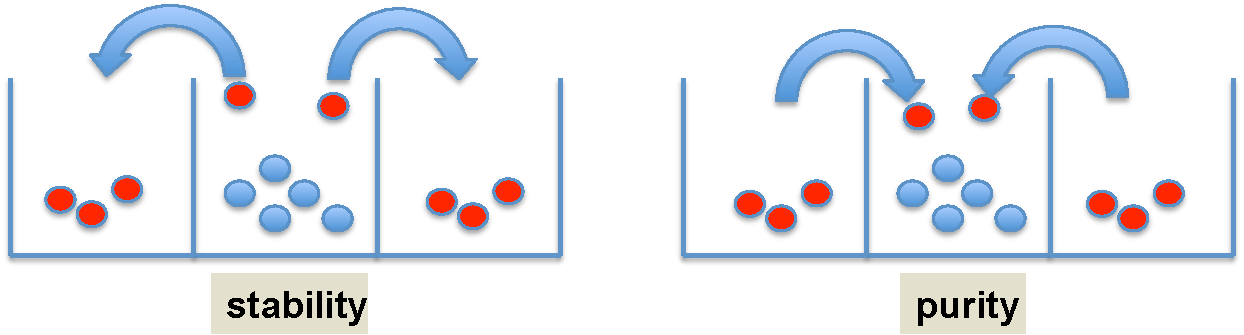
\includegraphics[width=0.8\textwidth]{Chapters/04_Analysis/04b_XSections/images/purity_and_stability.pdf}
     \caption[Graphical representation of bin purity and stability.]{Stability quantifies the migration of
     events out of a bin while purity quantifies the migration of events into a bin. Both quantities compare
     the bin in which an event is generated to the range in which they are reconstructed.}
     \label{fig:purity_and_stability}
 \end{figure}

In this analysis, the bins for each primary variable distribution were chosen such that all bins have purity
and stability values of 0.5 or greater, meaning that at least half of the events generated in a bin remain in
that bin after reconstruction, and that at least half of the events reconstructed in a bin were generated in
that bin. In order to avoid very small bins with a large relative statistical error, a requirement that all
bins have at least 100 events is also enforced.

The determination of the bin boundaries following these criteria is carried out simultaneously in (and
therefore the binning is identical in) both centre of mass energies and both the electron+jets and
muon+jets channel.

Plots of generated versus reconstructed events in simulation for all primary variables are shown in the
electron+jets channel in Figure~\ref{fig:binning_7TeV_electron} for $\roots=7\TeV$ and in
Figure~\ref{fig:binning_8TeV_electron} for $\roots=8\TeV$. The corresponding plots in the muon+jets channel
are shown in Figures~\ref{fig:binning_7TeV_muon} and \ref{fig:binning_8TeV_muon} in
Appendix~\ref{as:binning_muon}. %The purity and stability values of the chosen bins are shown in
%Appendix~\ref{as:binning_tables_electron}.

\begin{figure}[hbtp]
	\centering
     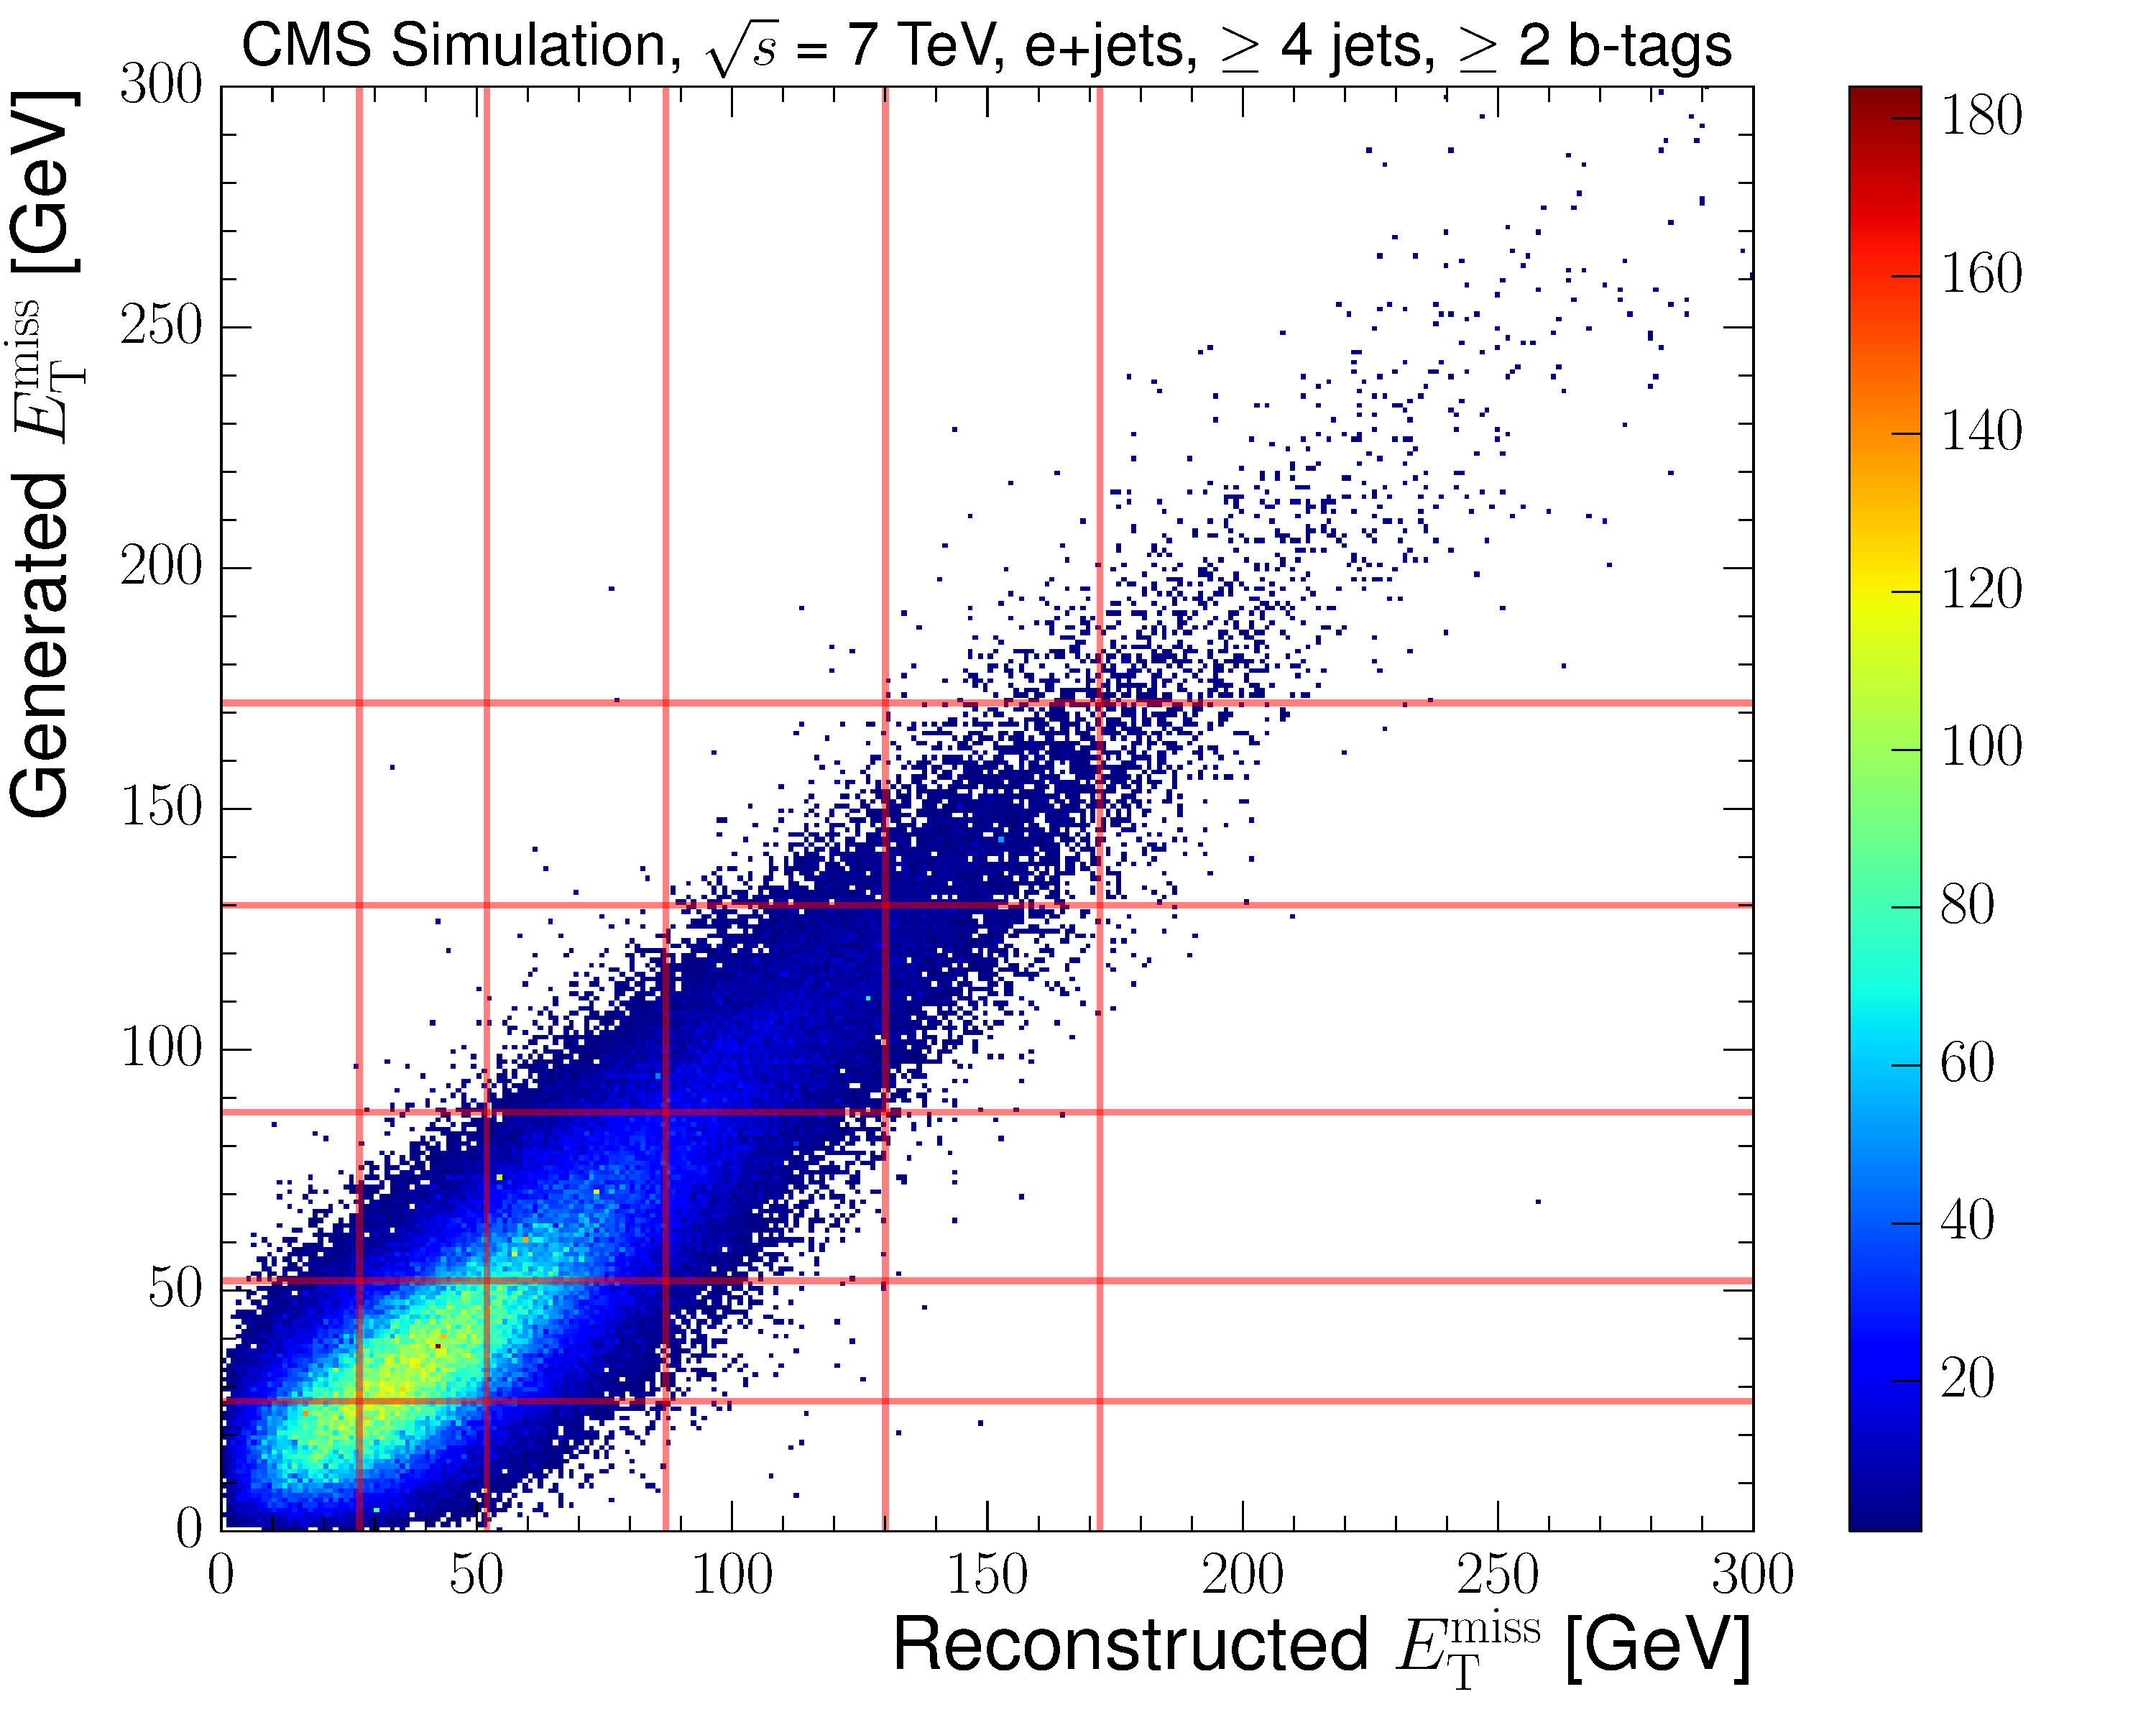
\includegraphics[width=0.48\textwidth]{Chapters/04_Analysis/04b_XSections/images/binning/electron_MET_7TeV.pdf}\hfill
     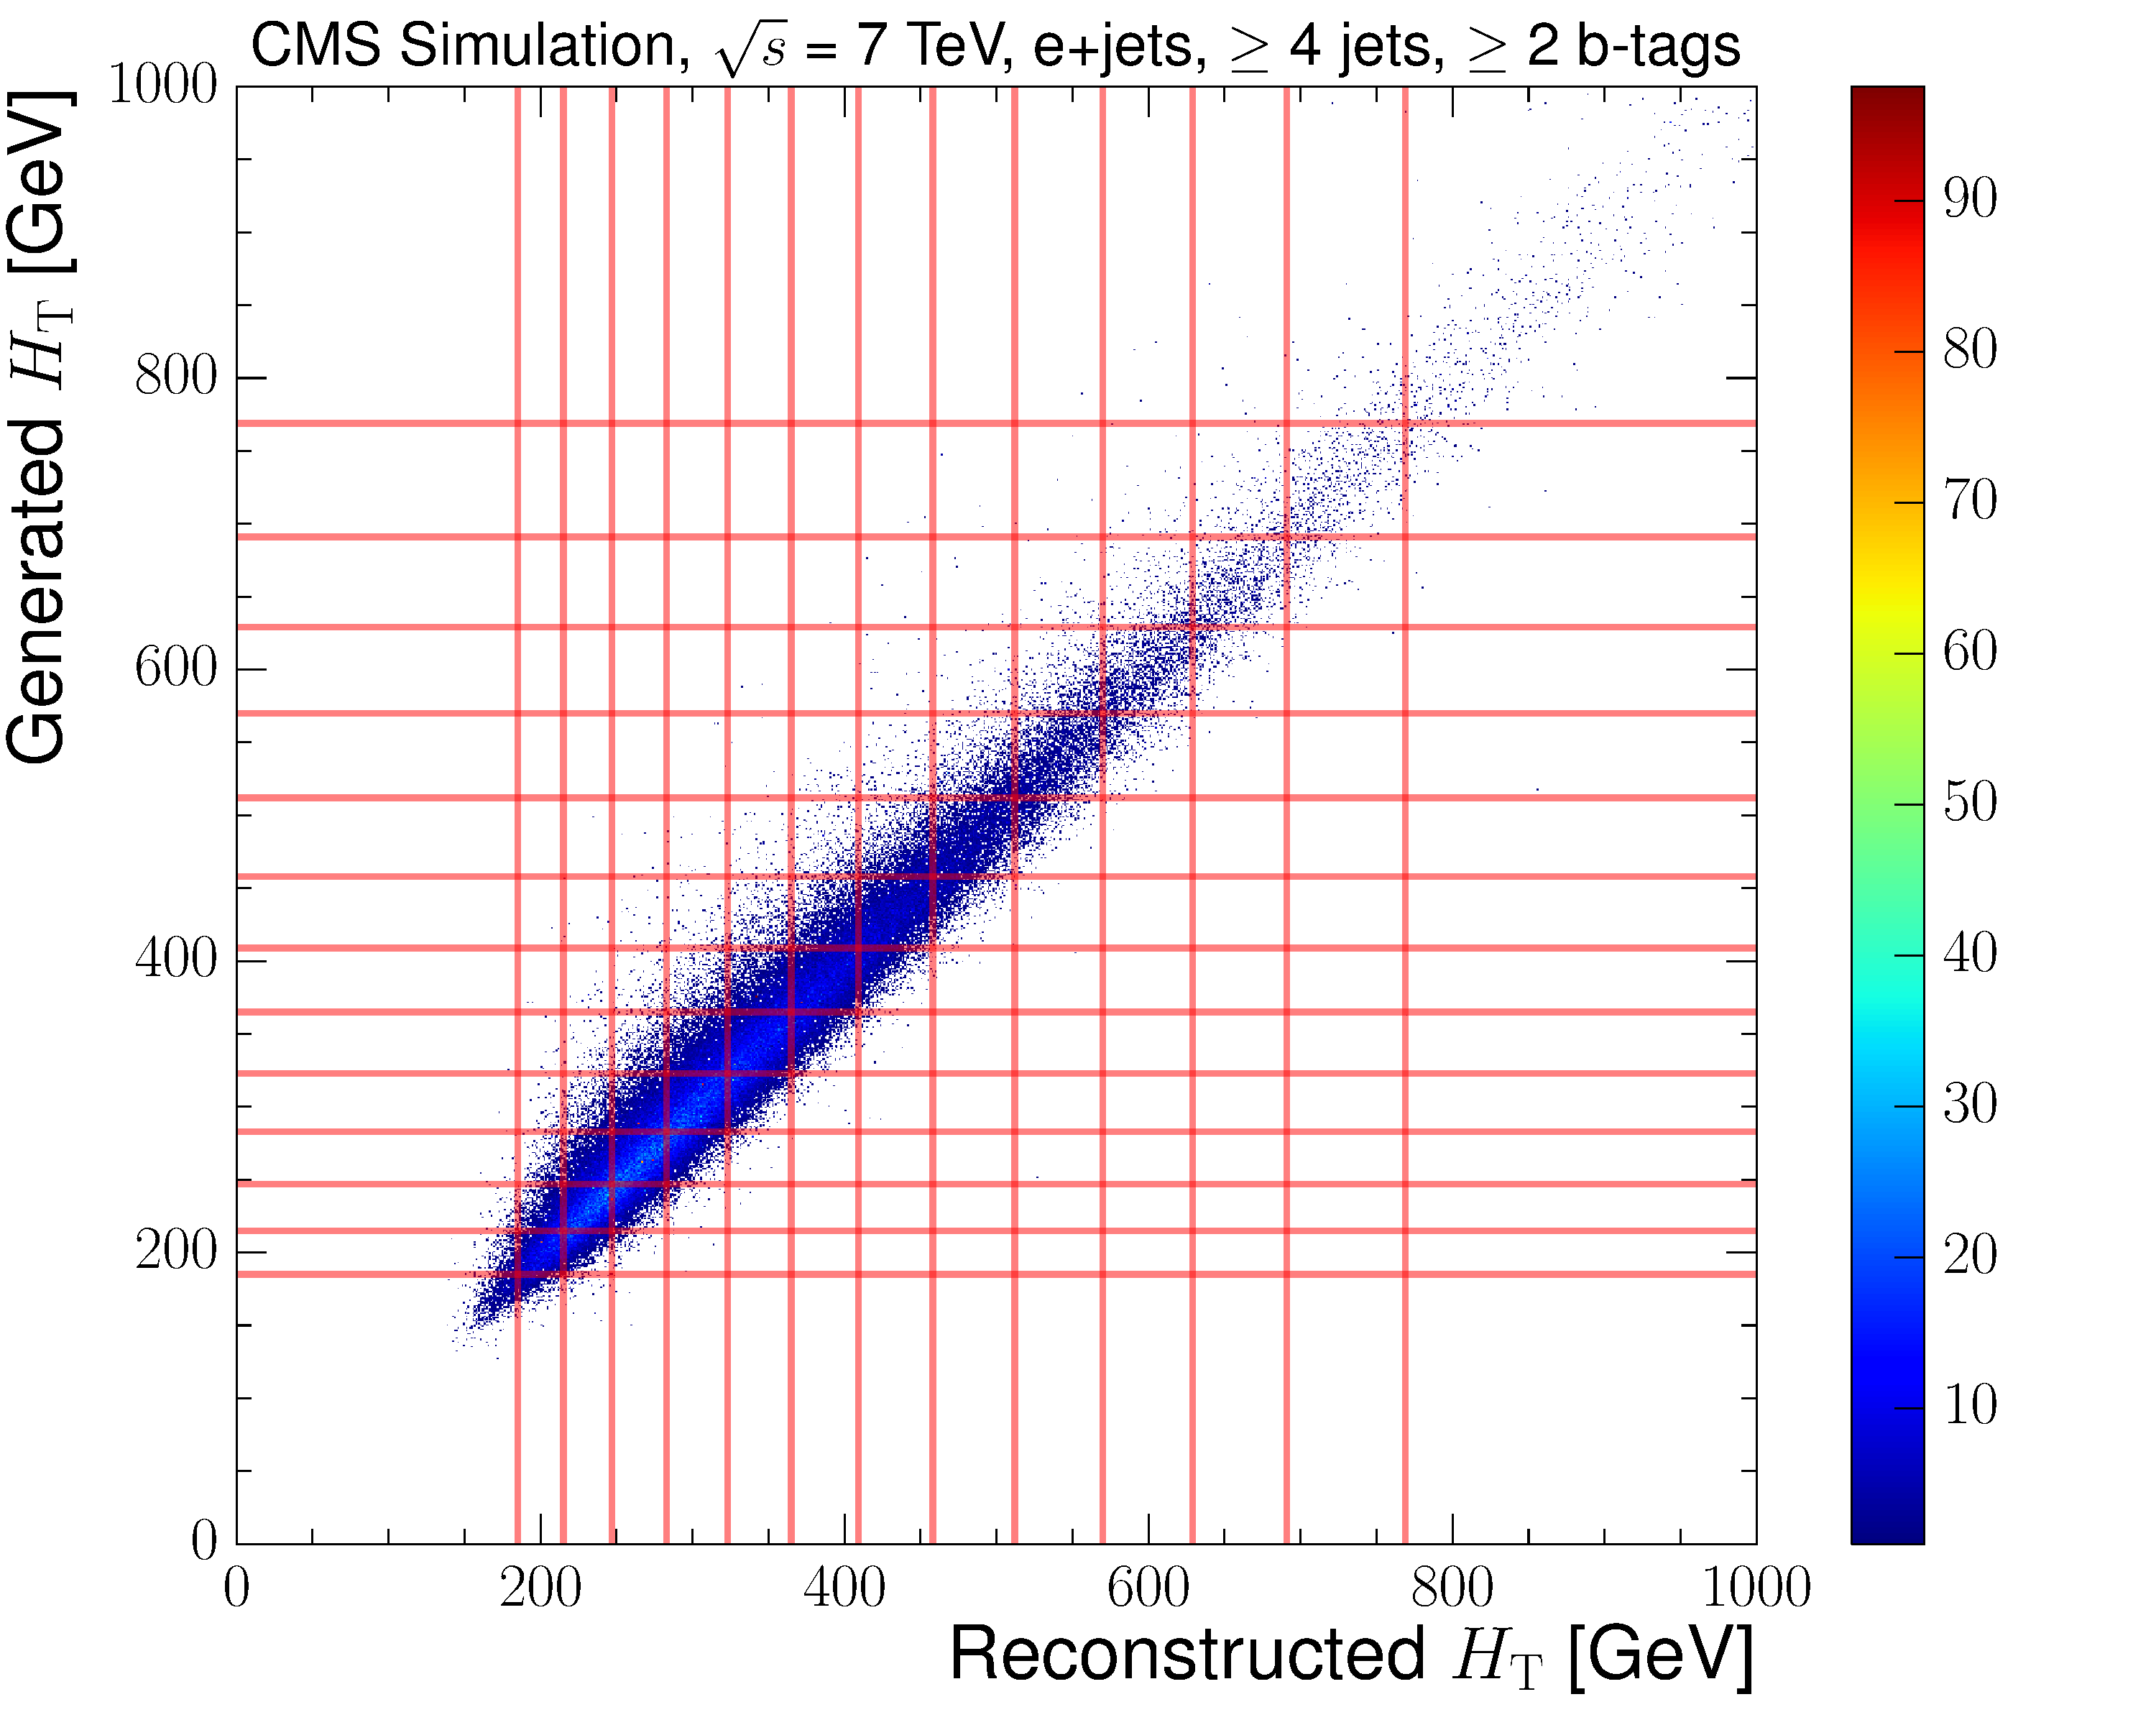
\includegraphics[width=0.48\textwidth]{Chapters/04_Analysis/04b_XSections/images/binning/electron_HT_7TeV.pdf}\\
     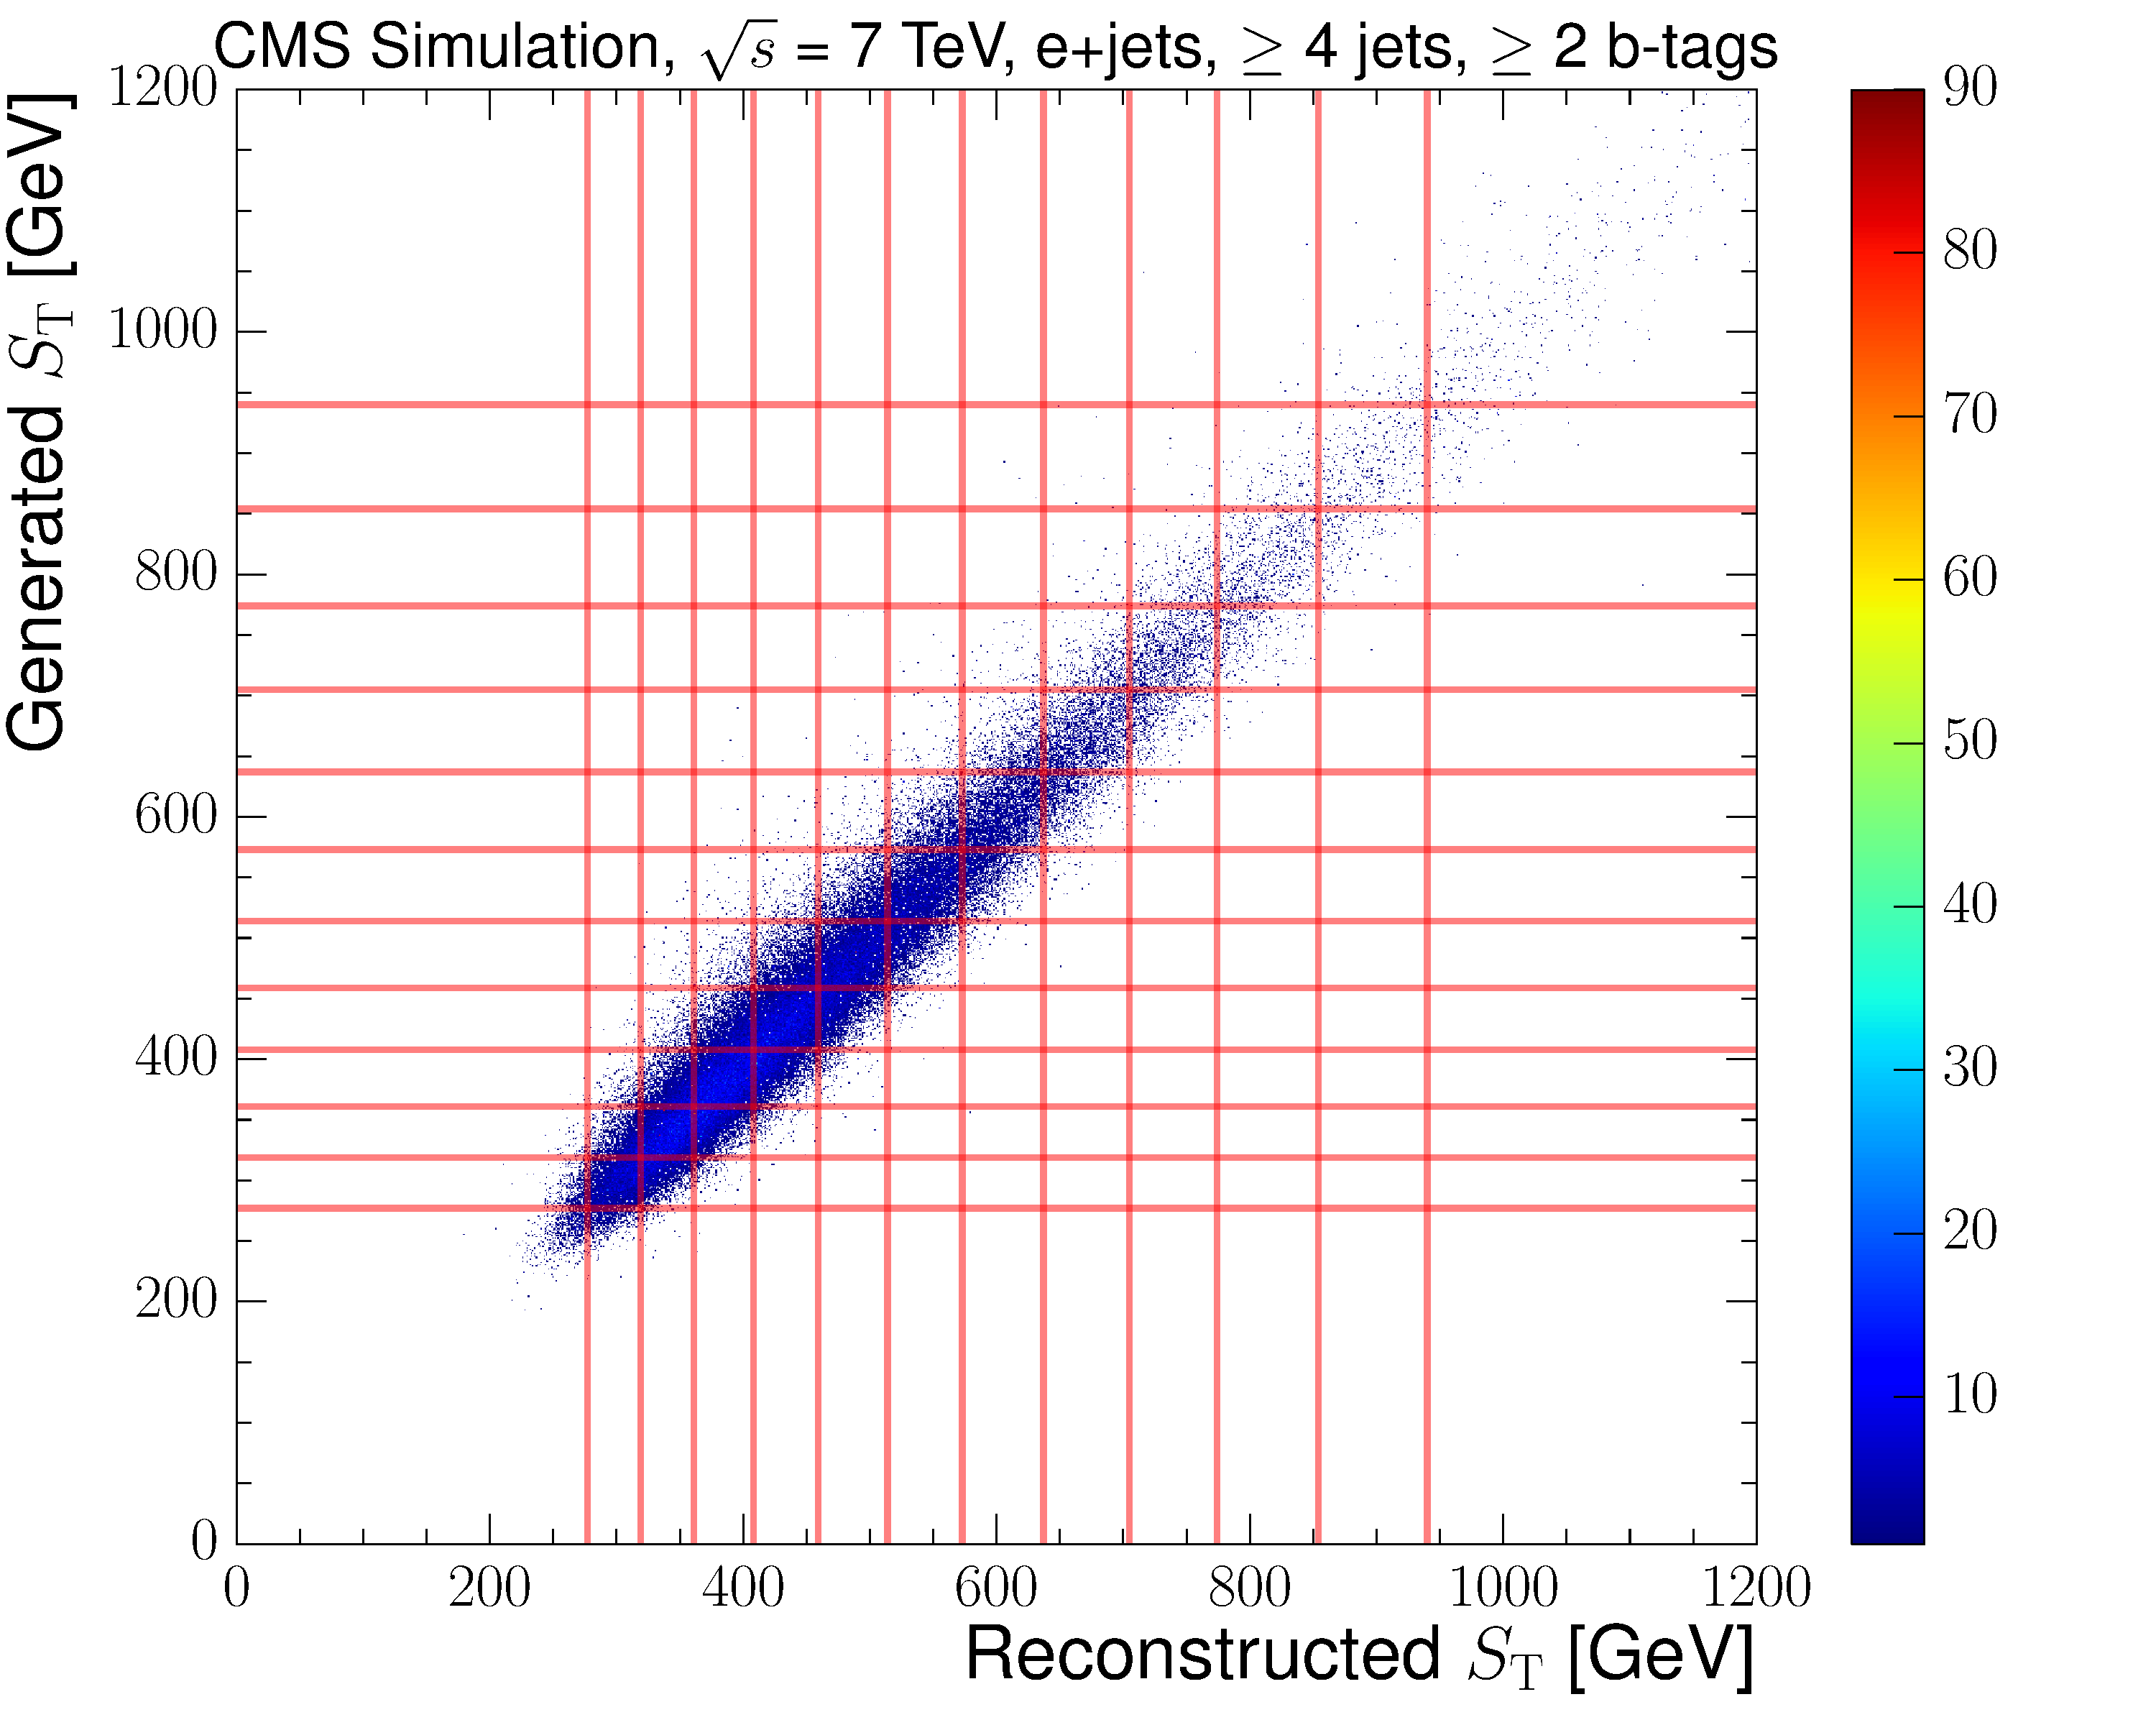
\includegraphics[width=0.48\textwidth]{Chapters/04_Analysis/04b_XSections/images/binning/electron_ST_7TeV.pdf}\hfill
     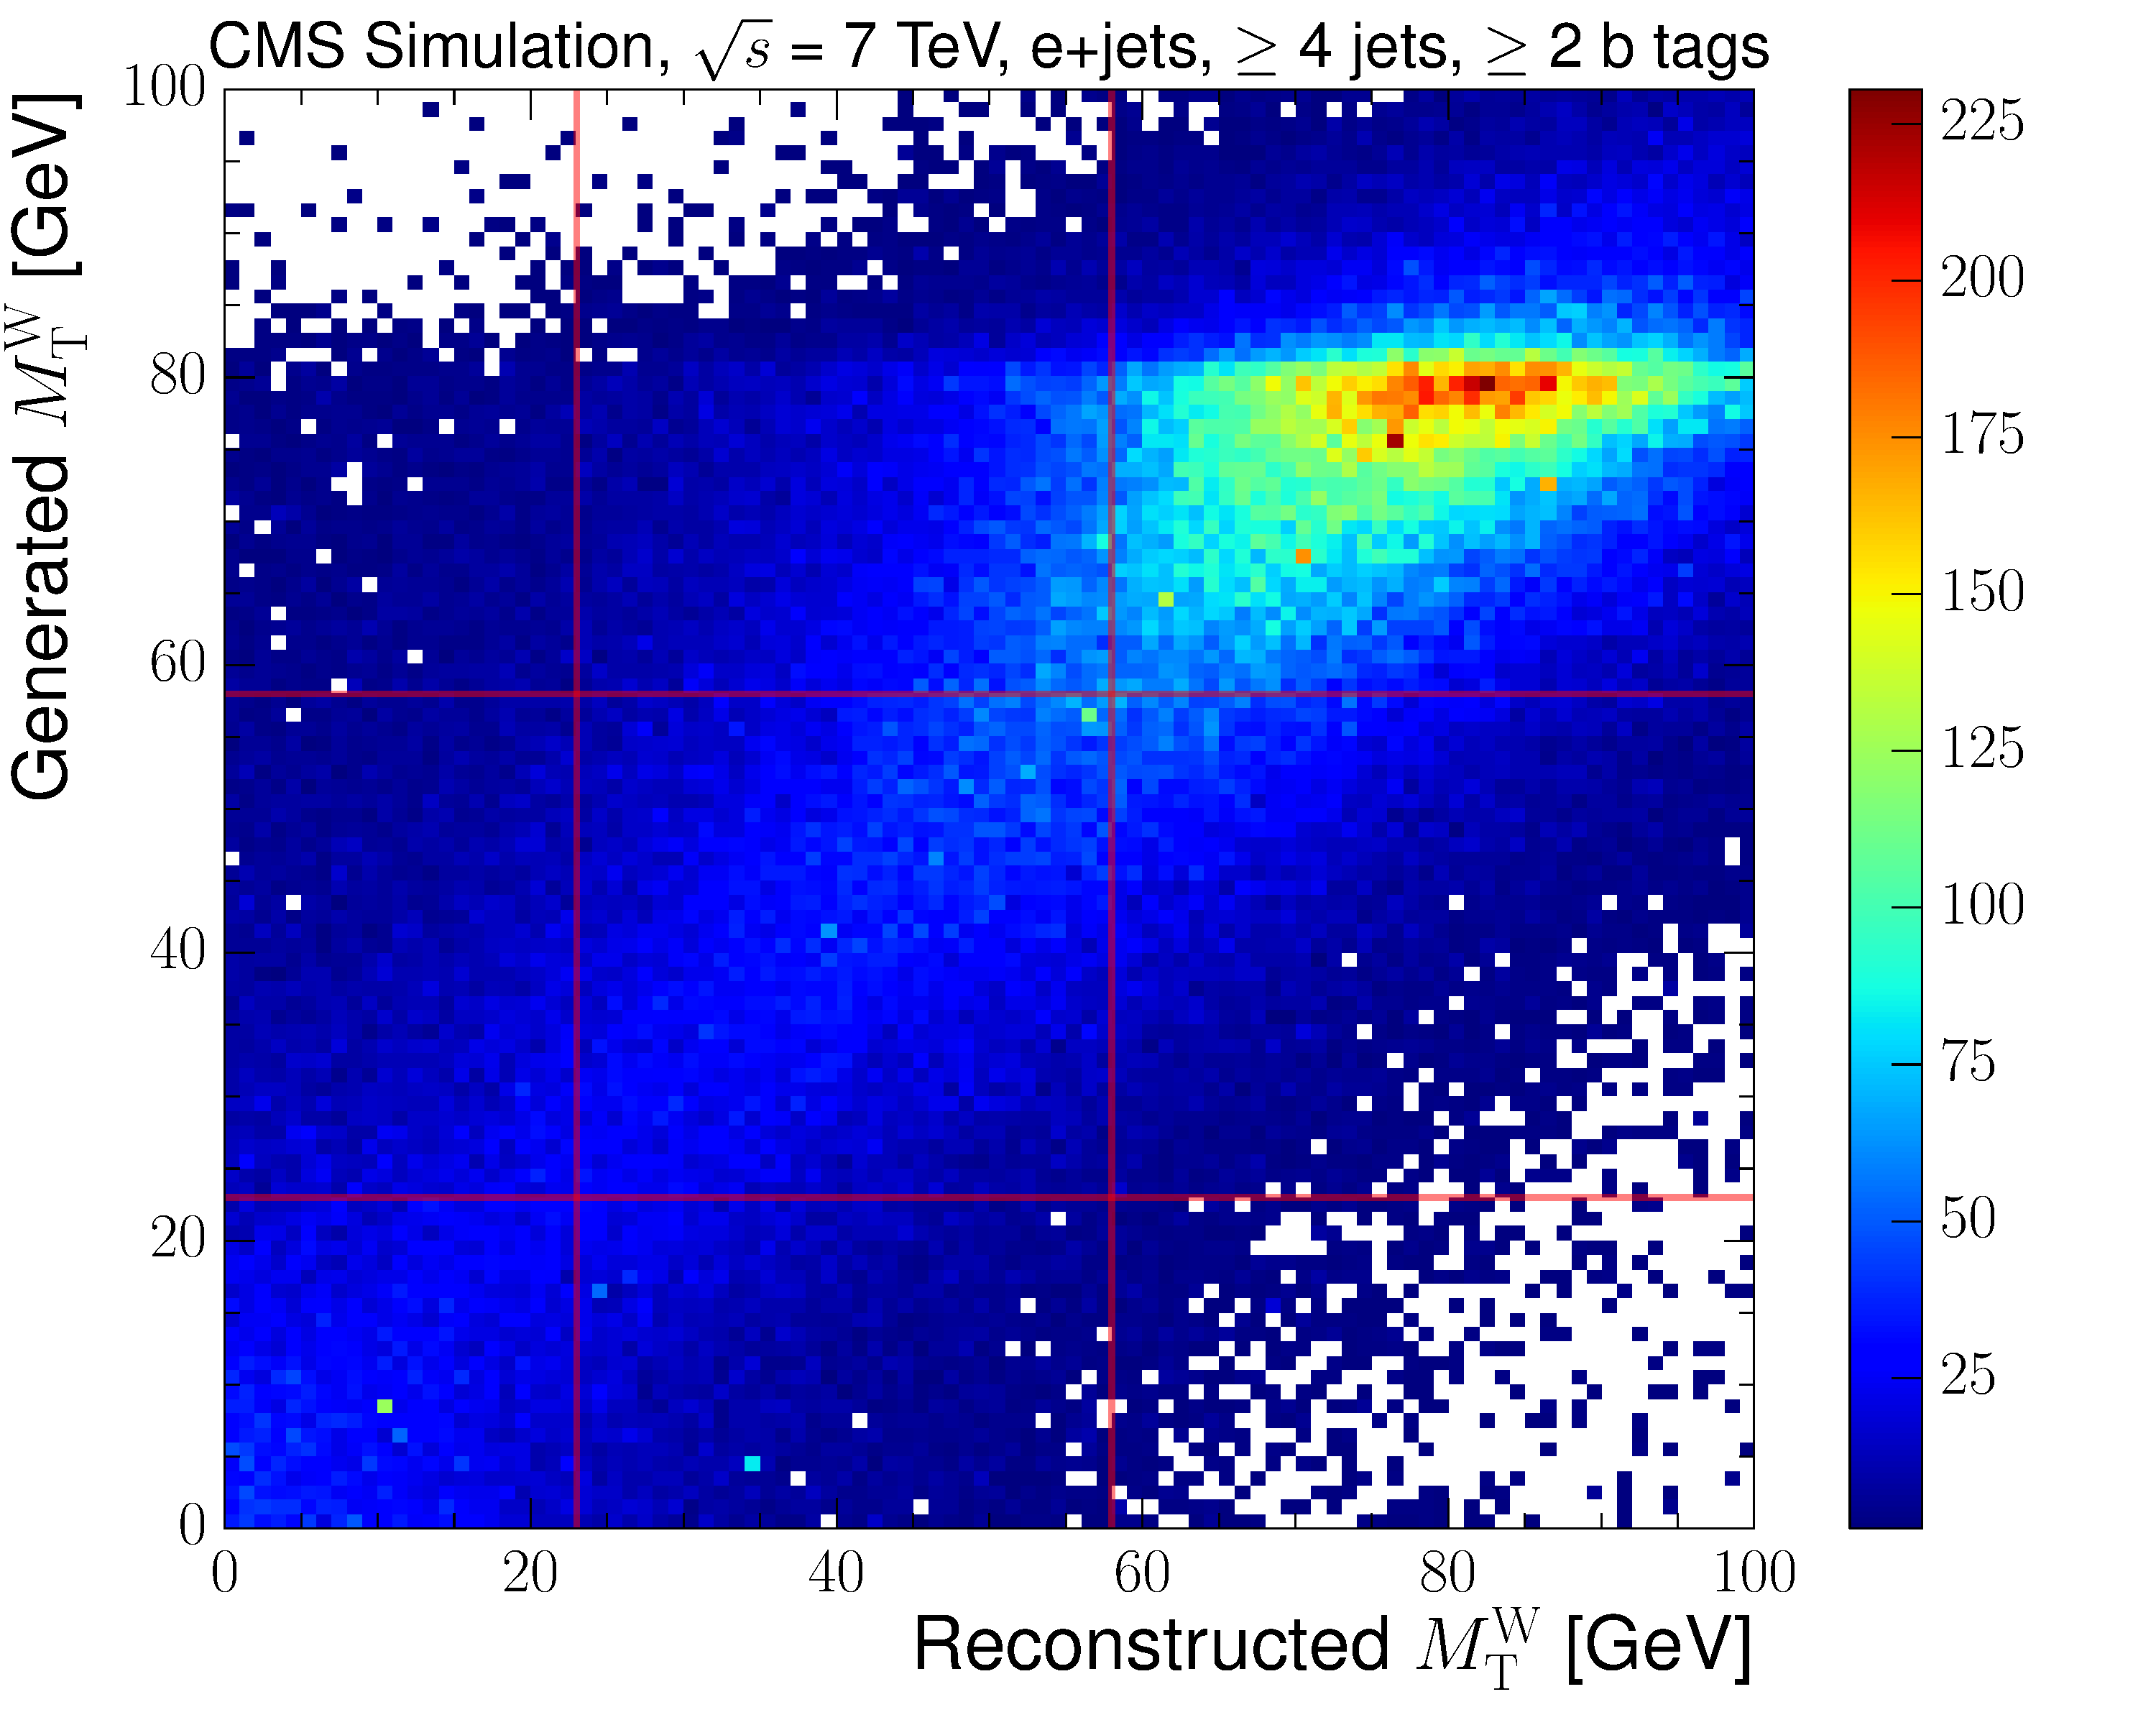
\includegraphics[width=0.48\textwidth]{Chapters/04_Analysis/04b_XSections/images/binning/electron_MT_7TeV.pdf}\\
	 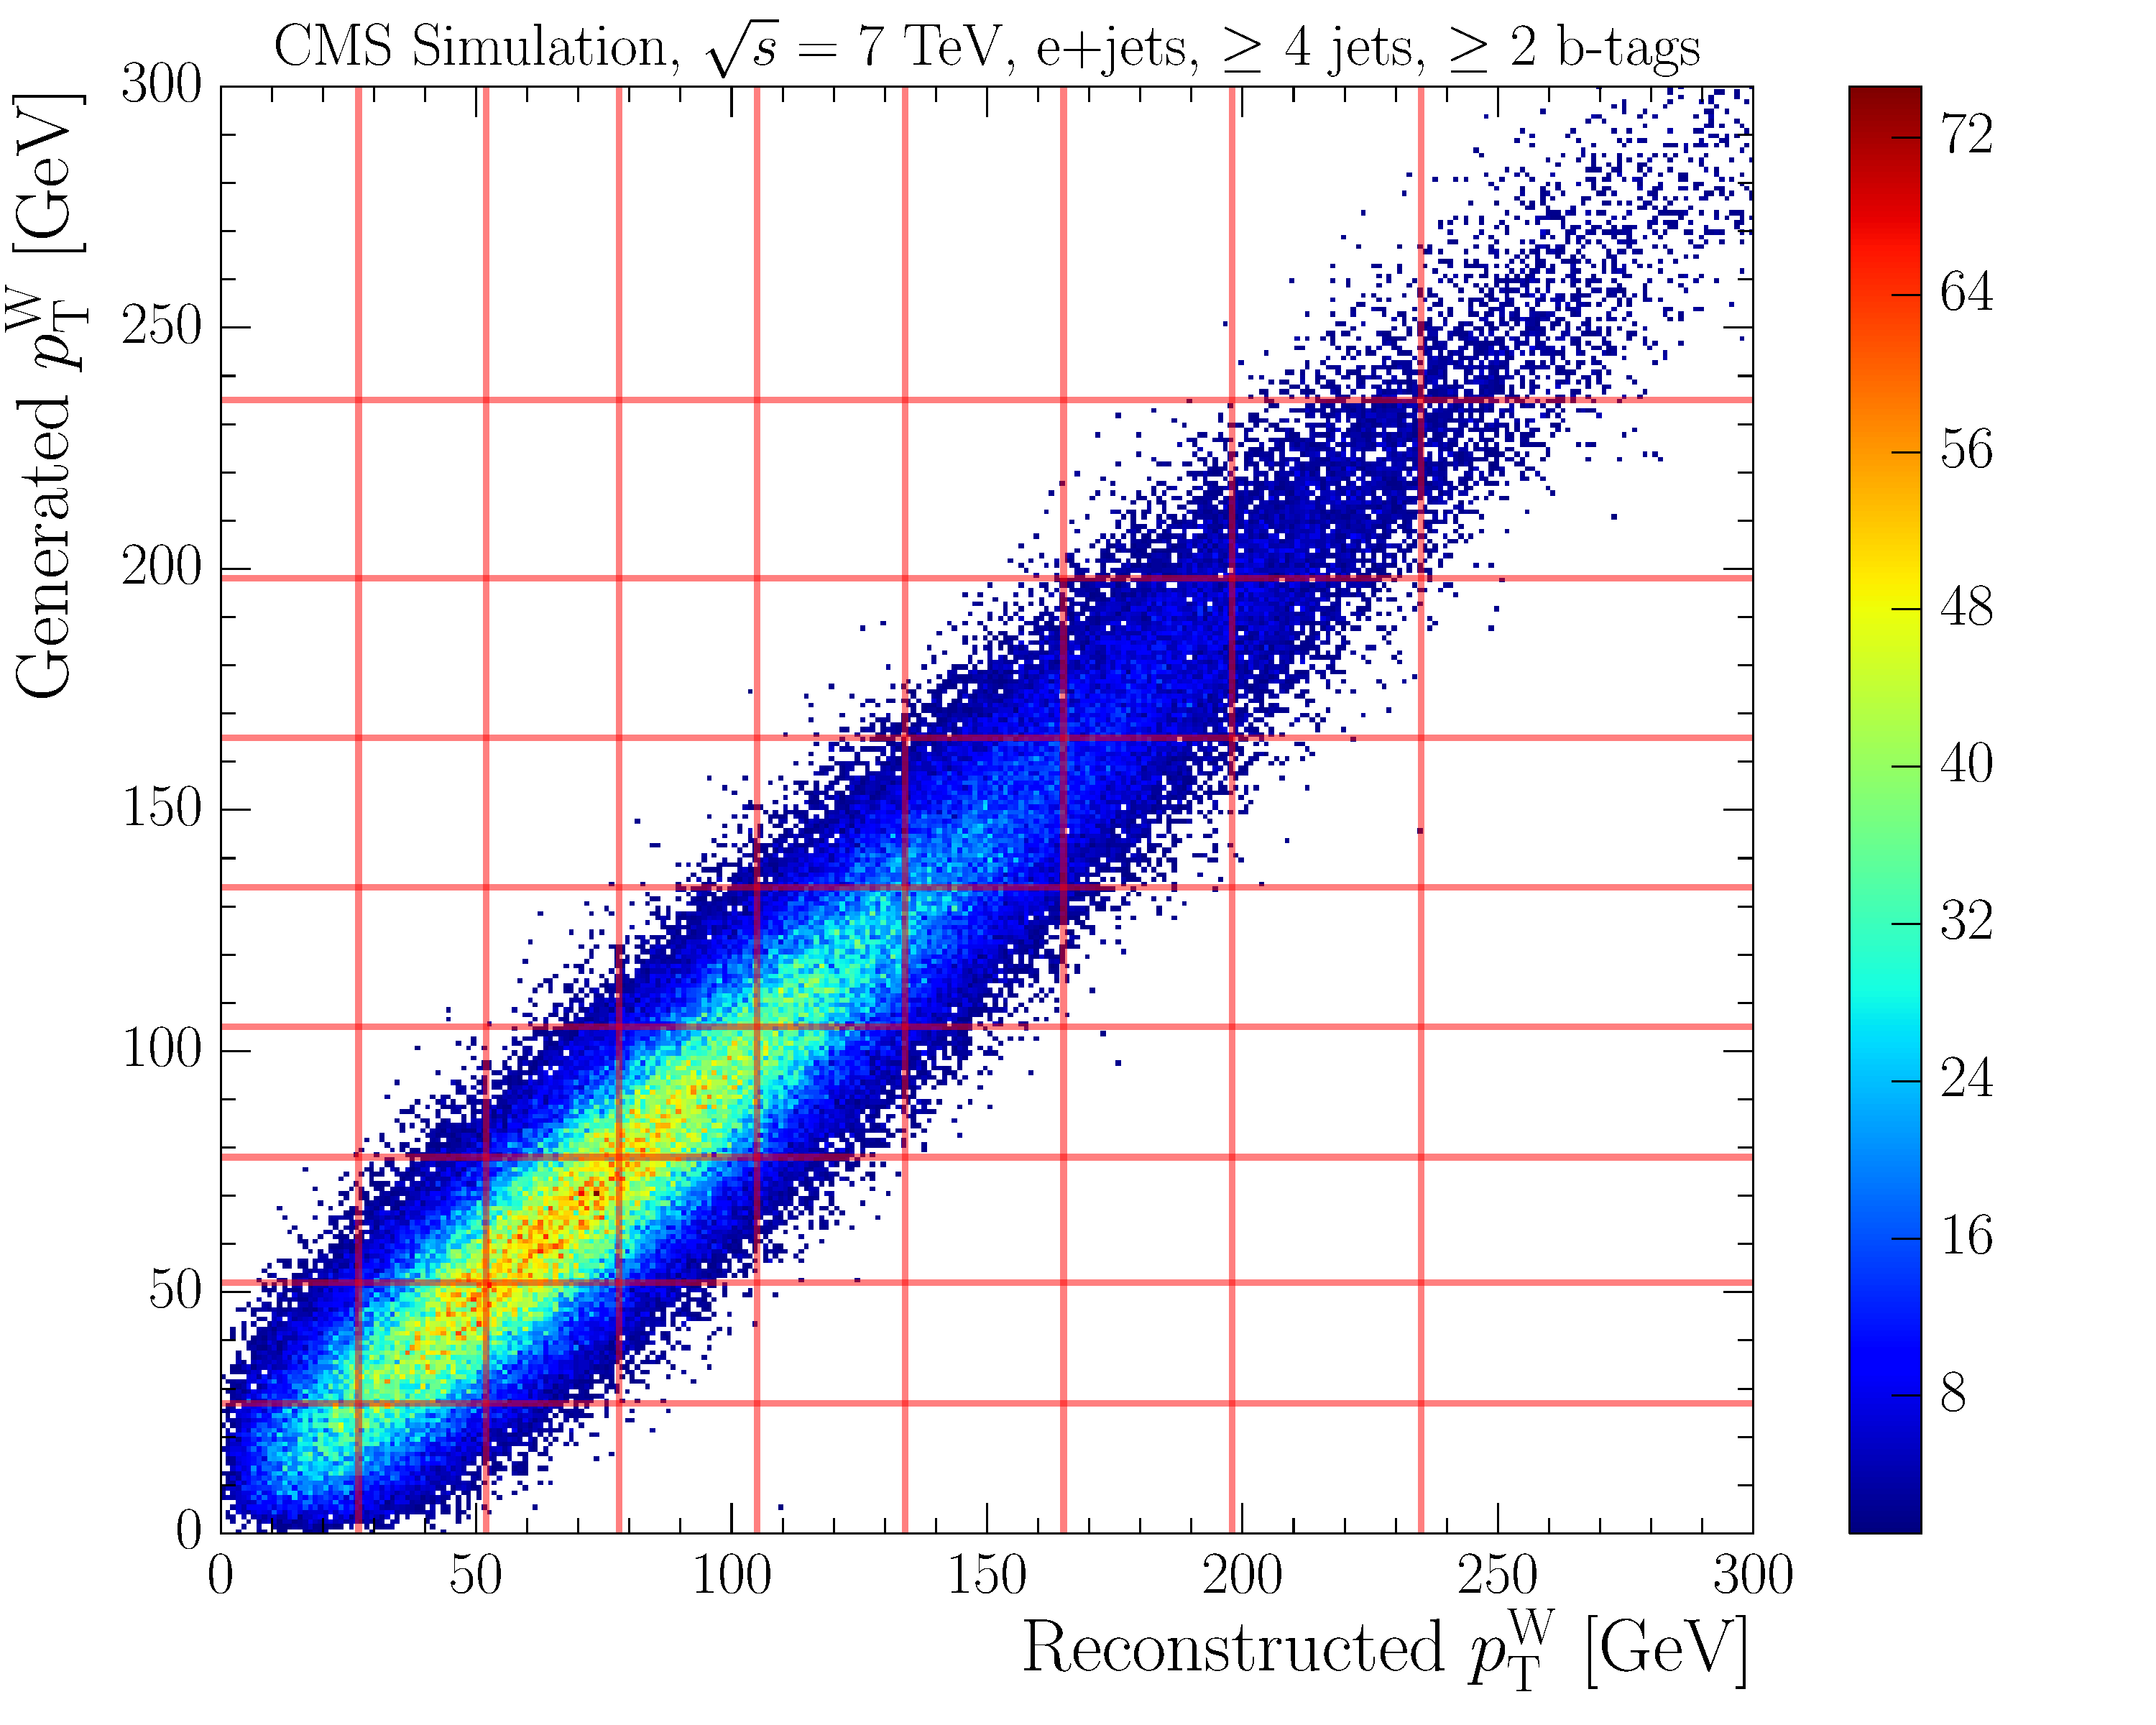
\includegraphics[width=0.48\textwidth]{Chapters/04_Analysis/04b_XSections/images/binning/electron_WPT_7TeV.pdf}\hfill
	 \caption[Generated versus reconstructed distributions of the primary variable at $\roots=7\TeV$.]{Generated
	 versus reconstructed distributions of the primary variables \met (upper left), \HT (upper right), \st (middle
	 left), \mt (middle right) and \wpt (lower) with horizontal and vertical lines representing the boundaries of
	 the selected bins at $\roots=7\TeV$ in the electron+ jets channel. These distributions are obtained using
	 \ttbar simulation.}
     \label{fig:binning_7TeV_electron}
\end{figure}

\begin{figure}[hbtp]
    \centering
     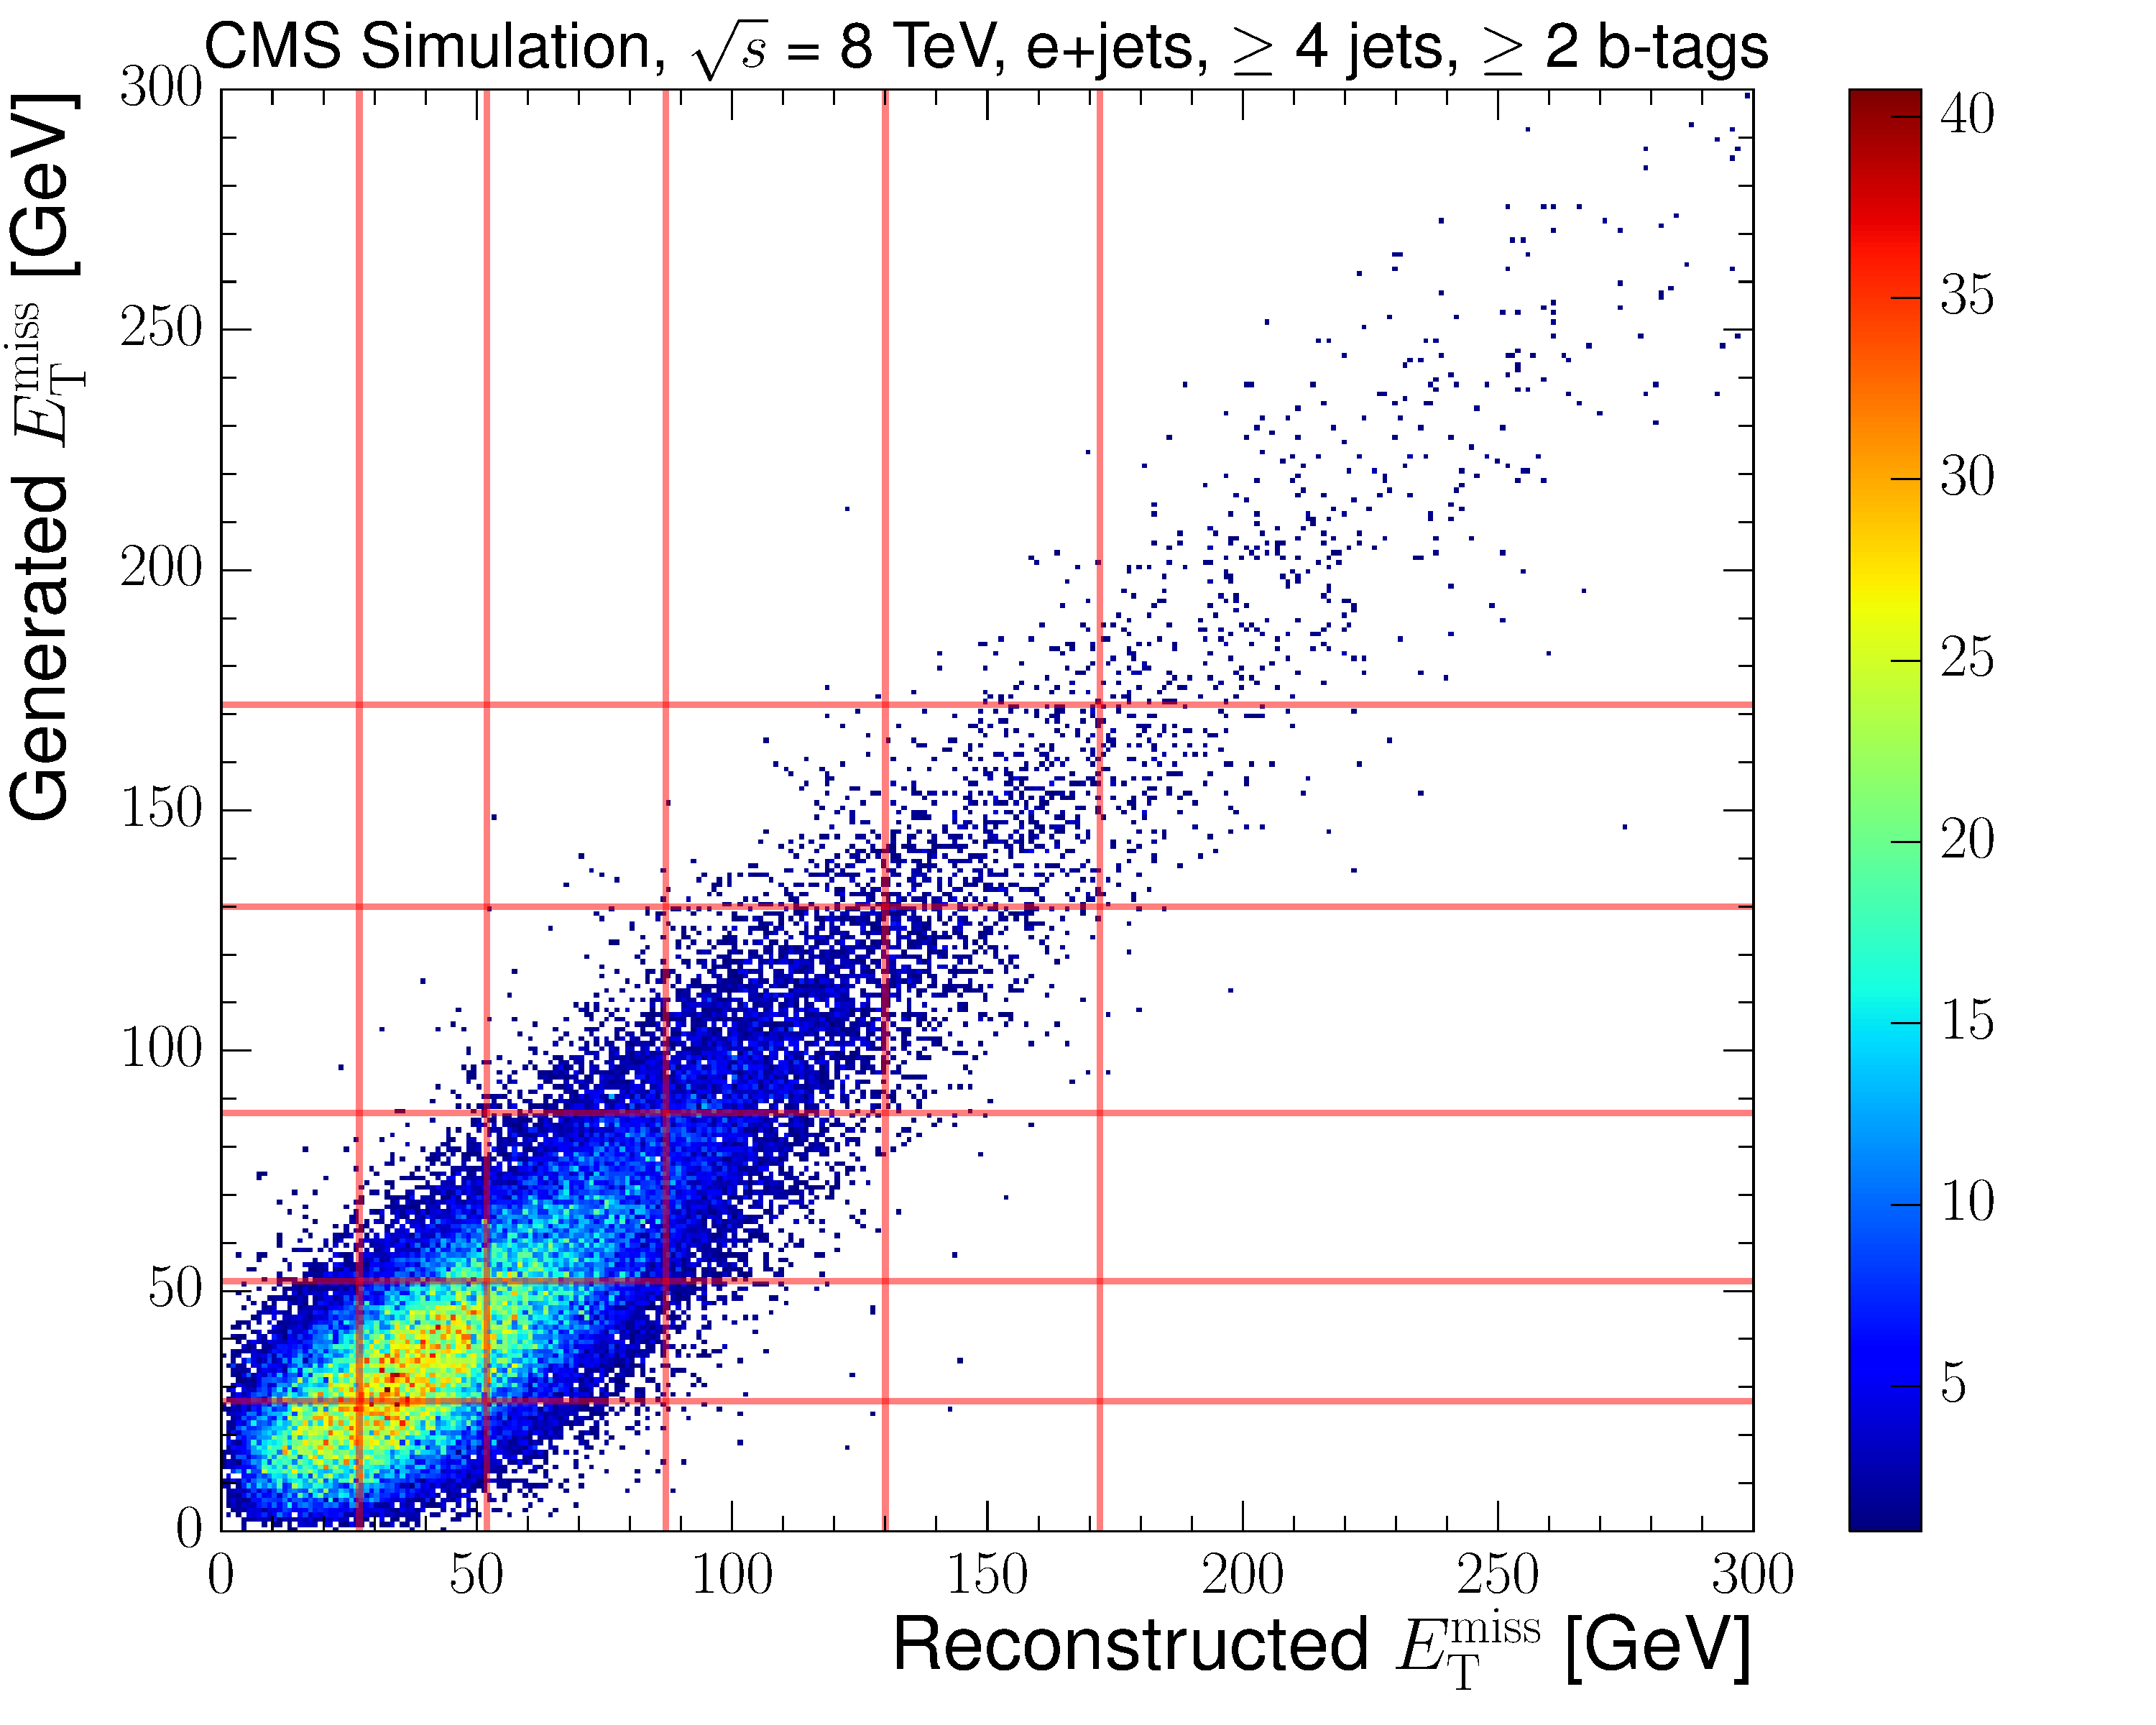
\includegraphics[width=0.48\textwidth]{Chapters/04_Analysis/04b_XSections/images/binning/electron_MET_8TeV.pdf}\hfill
     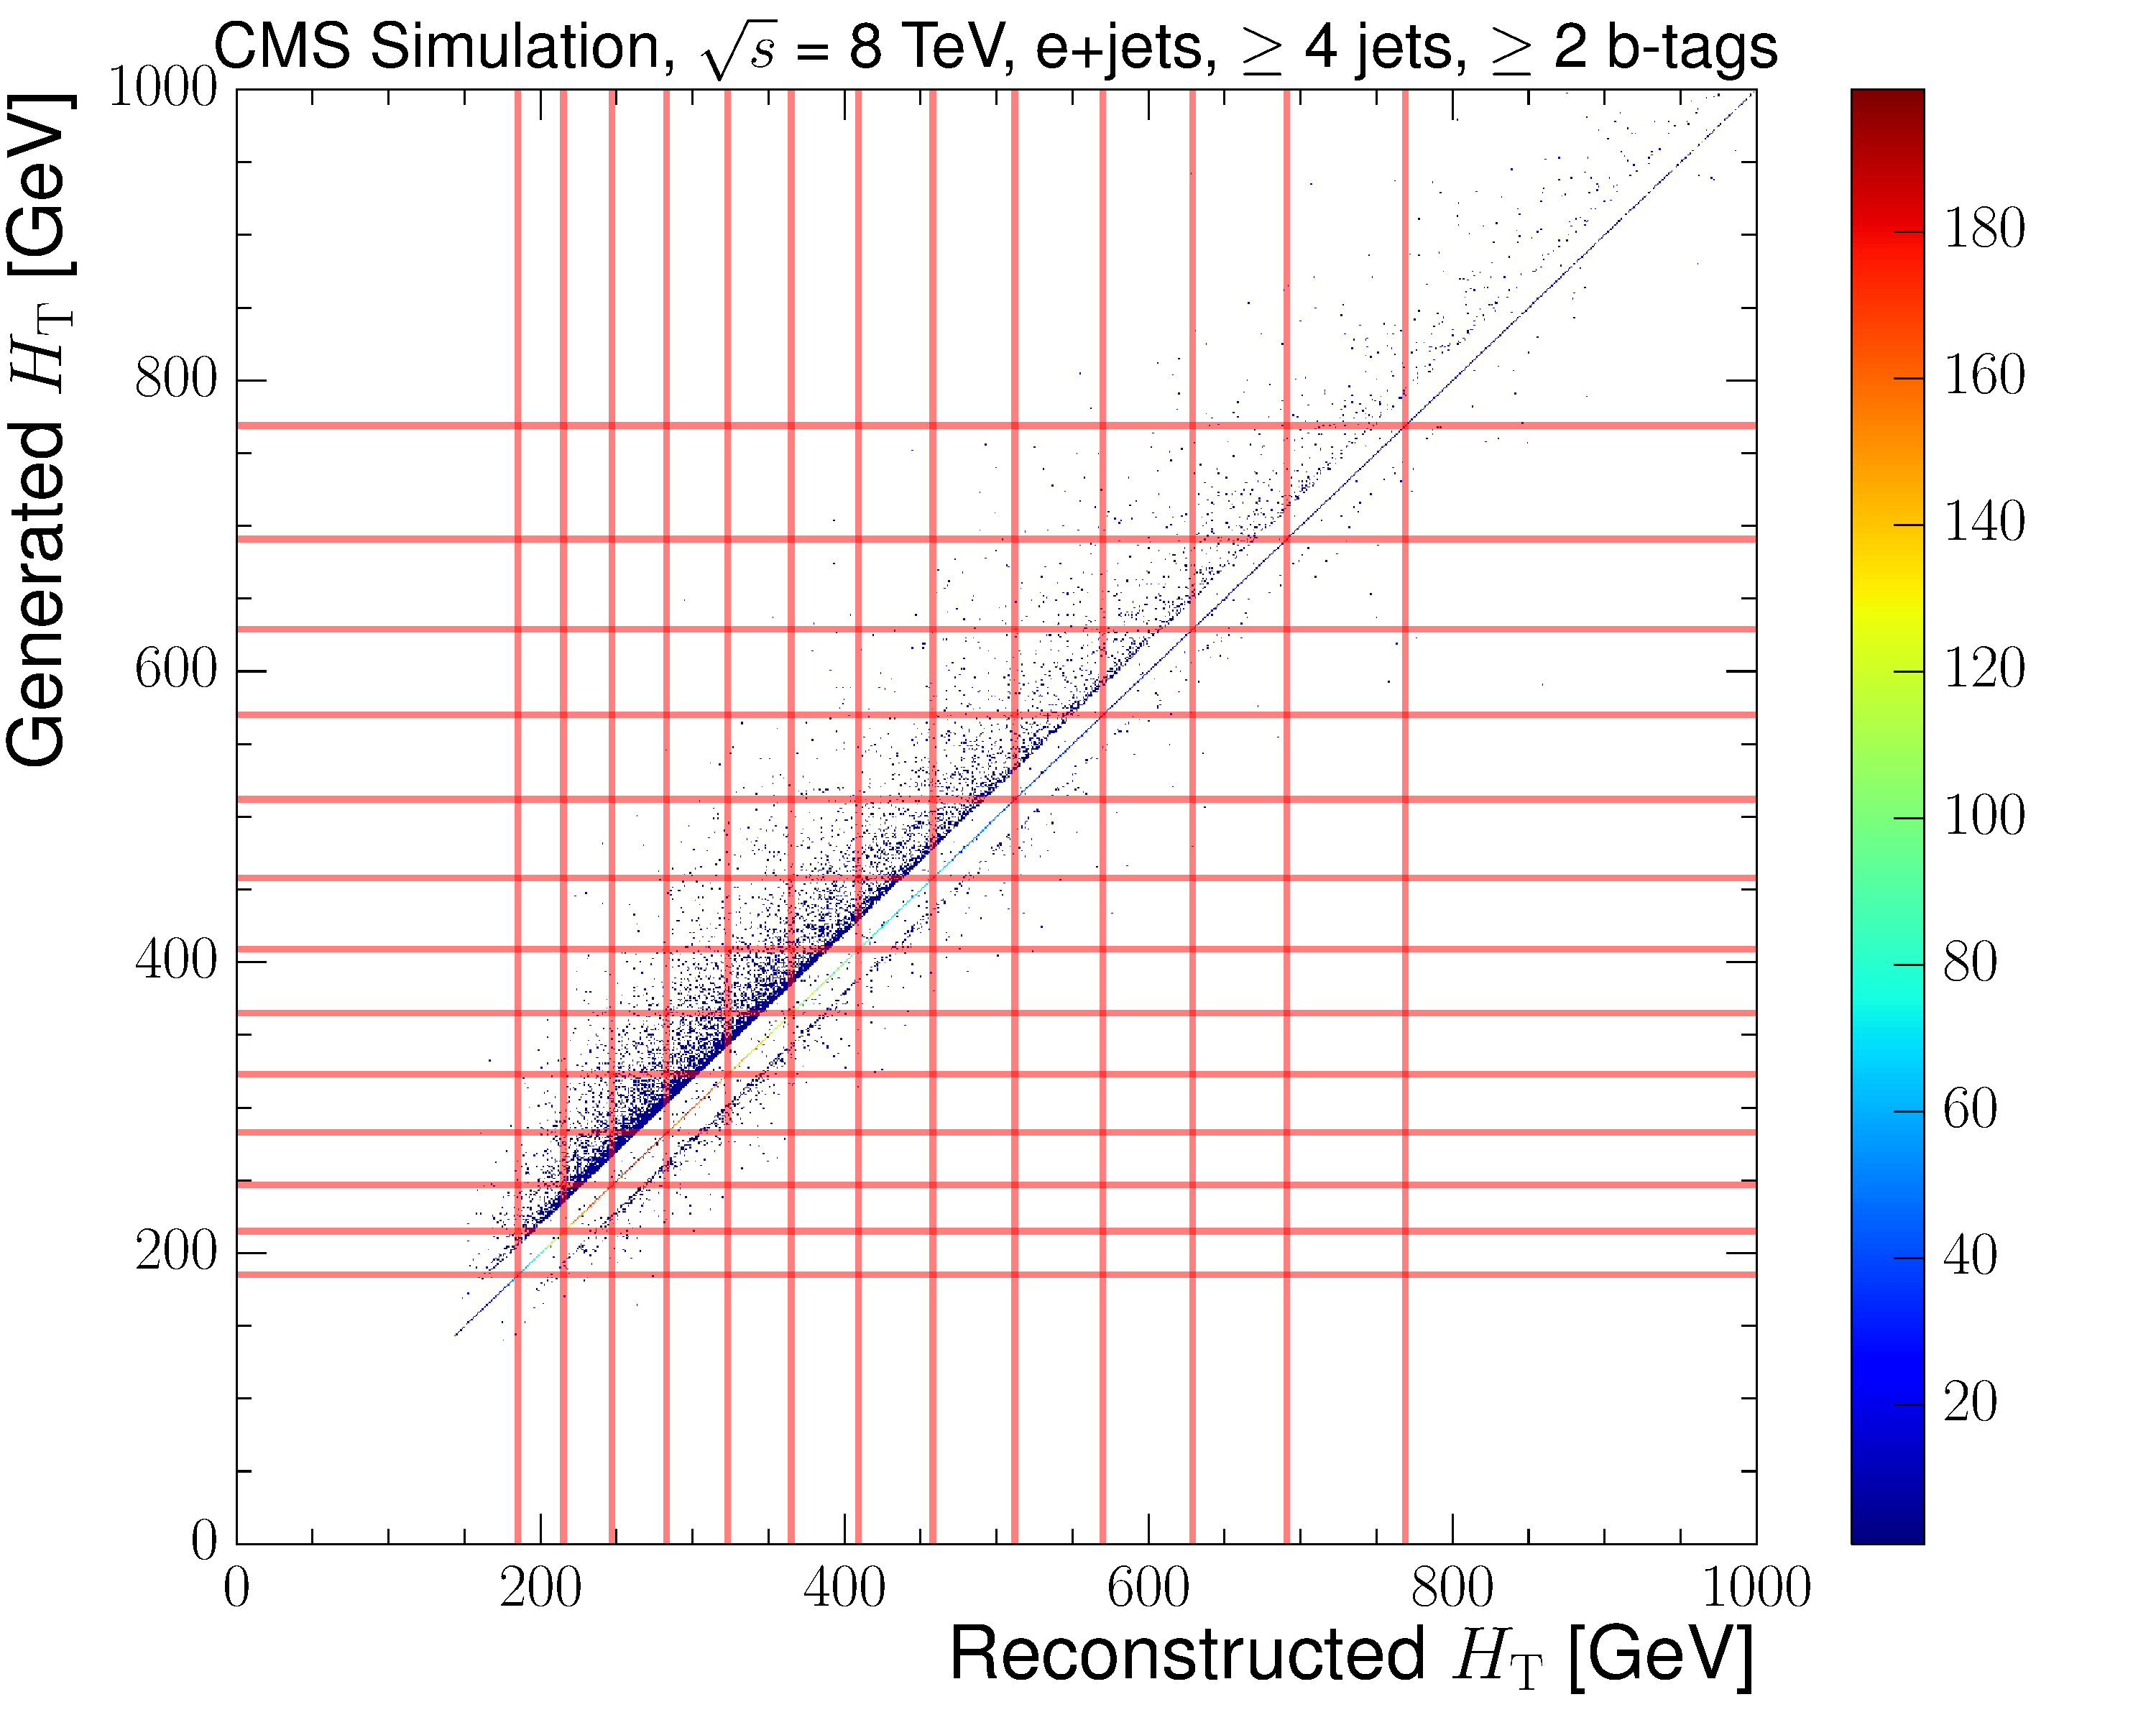
\includegraphics[width=0.48\textwidth]{Chapters/04_Analysis/04b_XSections/images/binning/electron_HT_8TeV.pdf}\\
     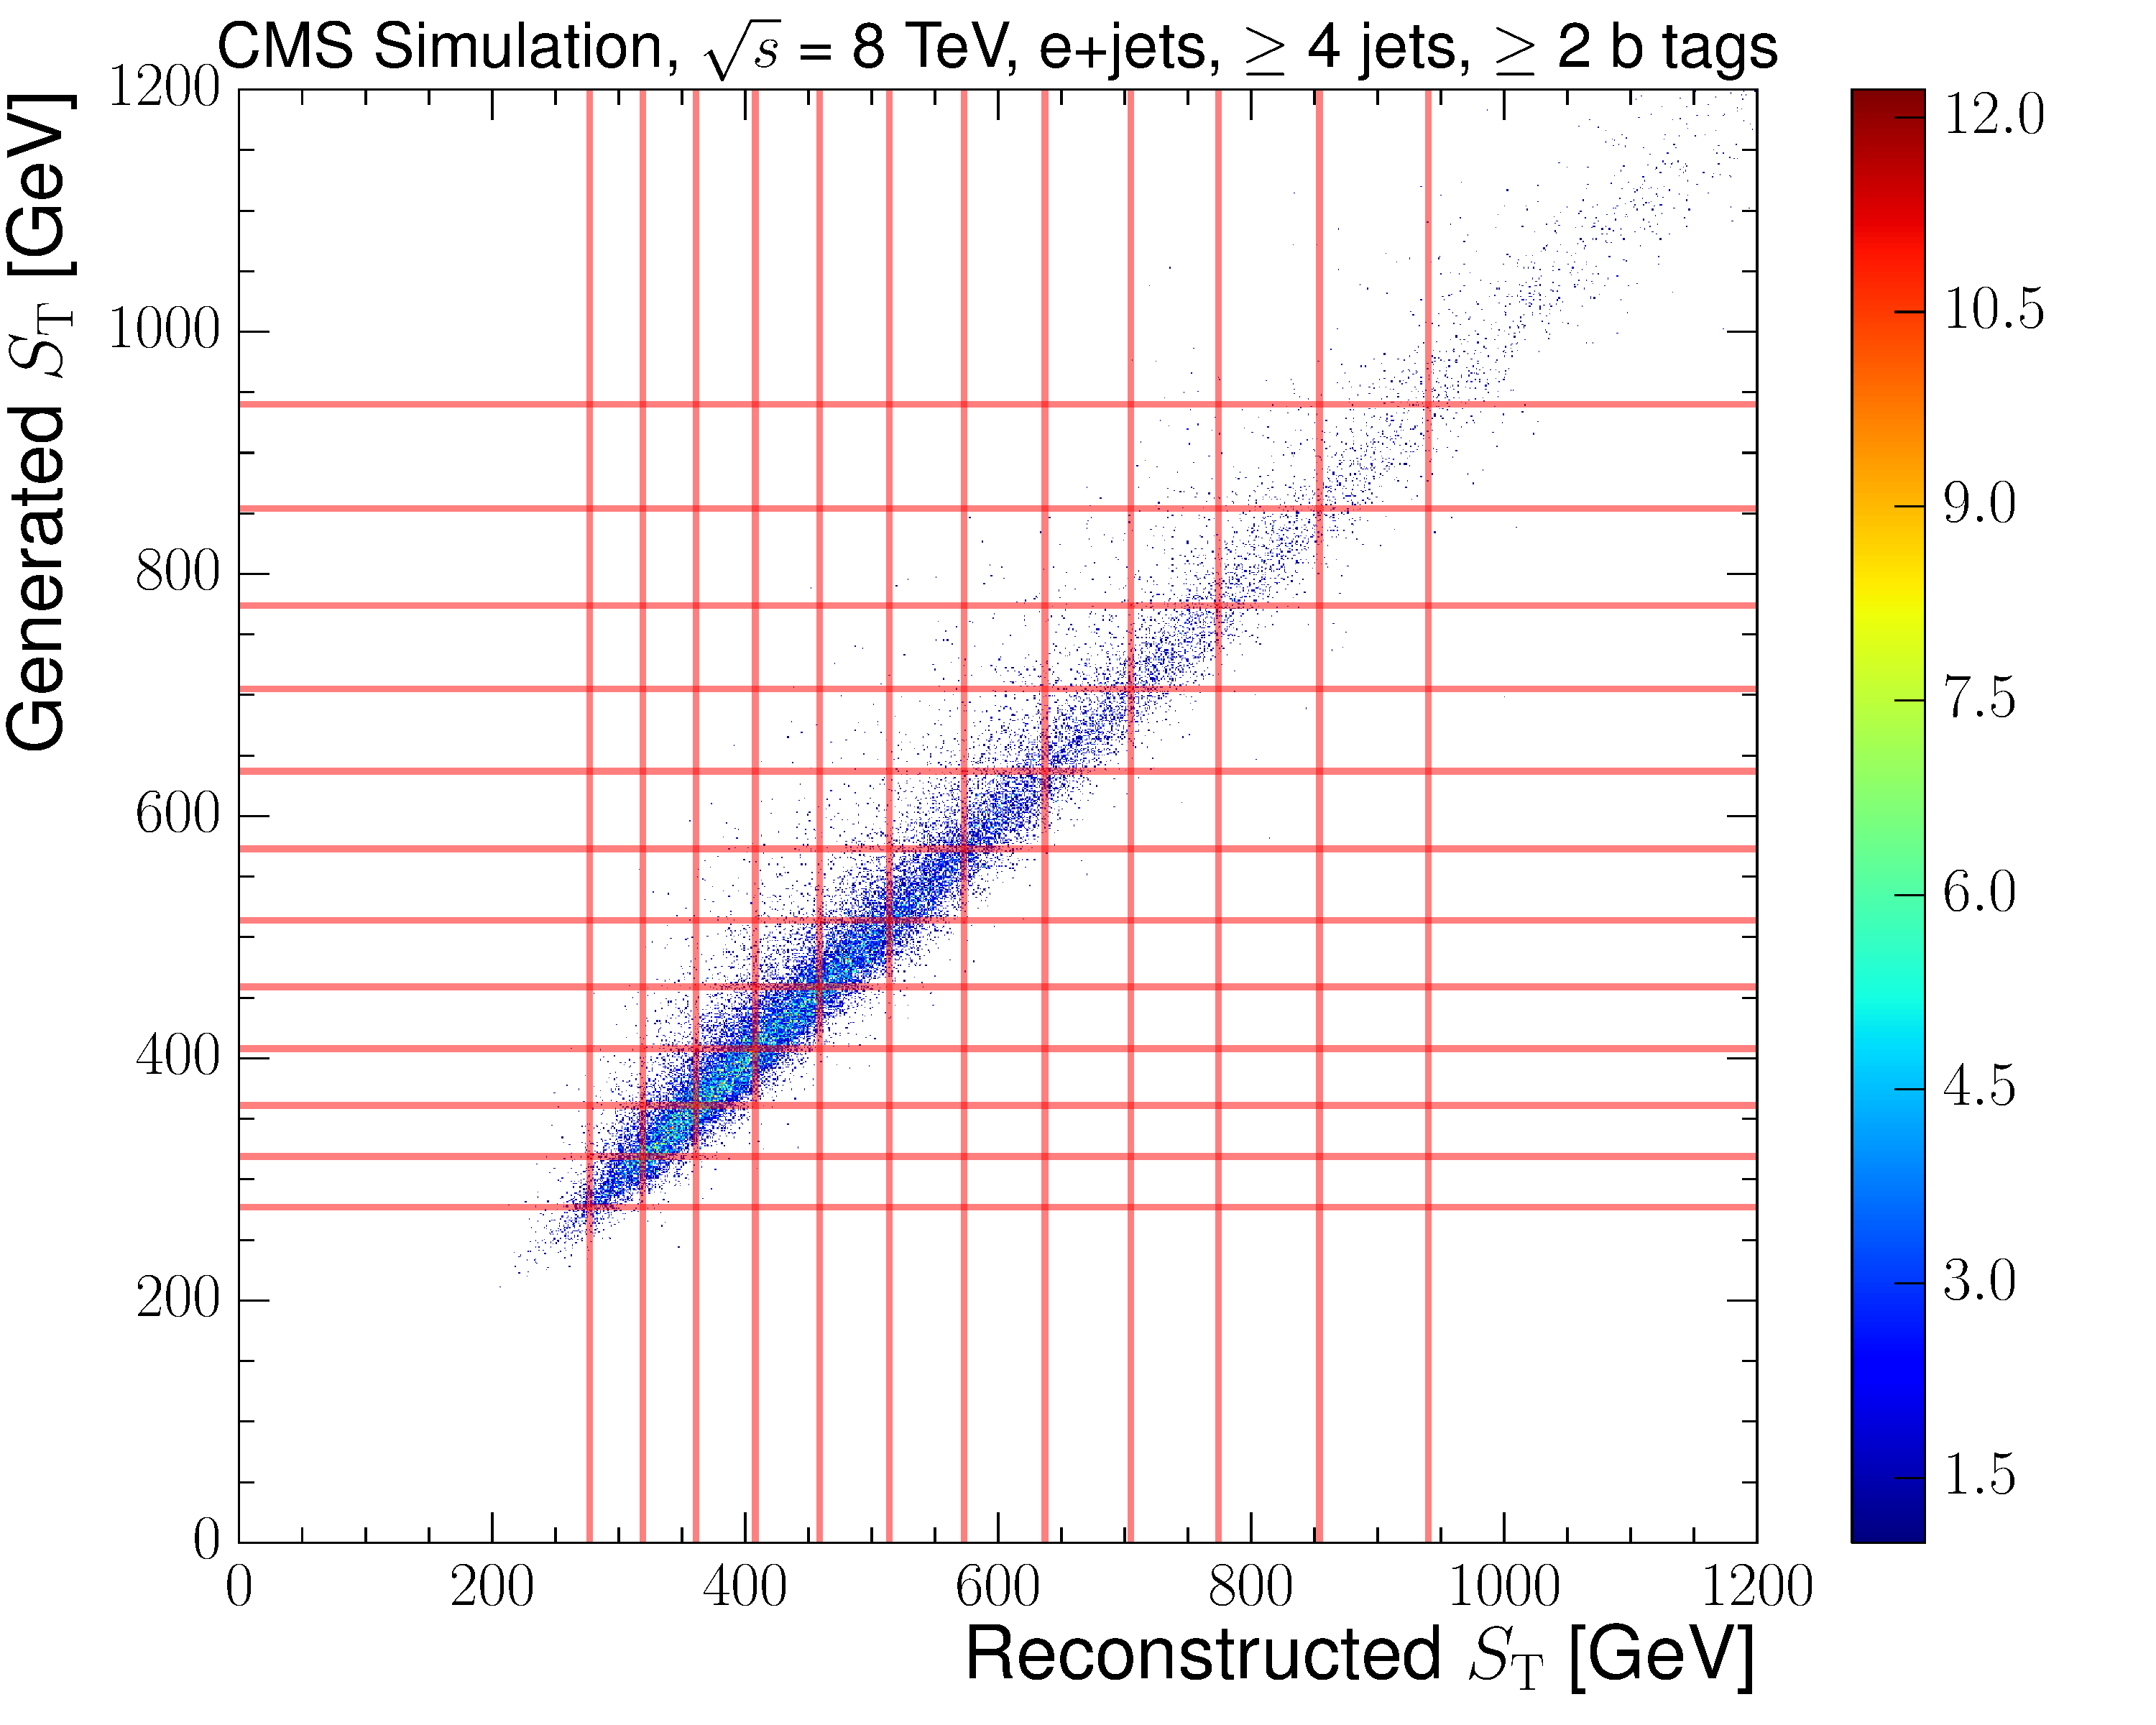
\includegraphics[width=0.48\textwidth]{Chapters/04_Analysis/04b_XSections/images/binning/electron_ST_8TeV.pdf}\hfill
     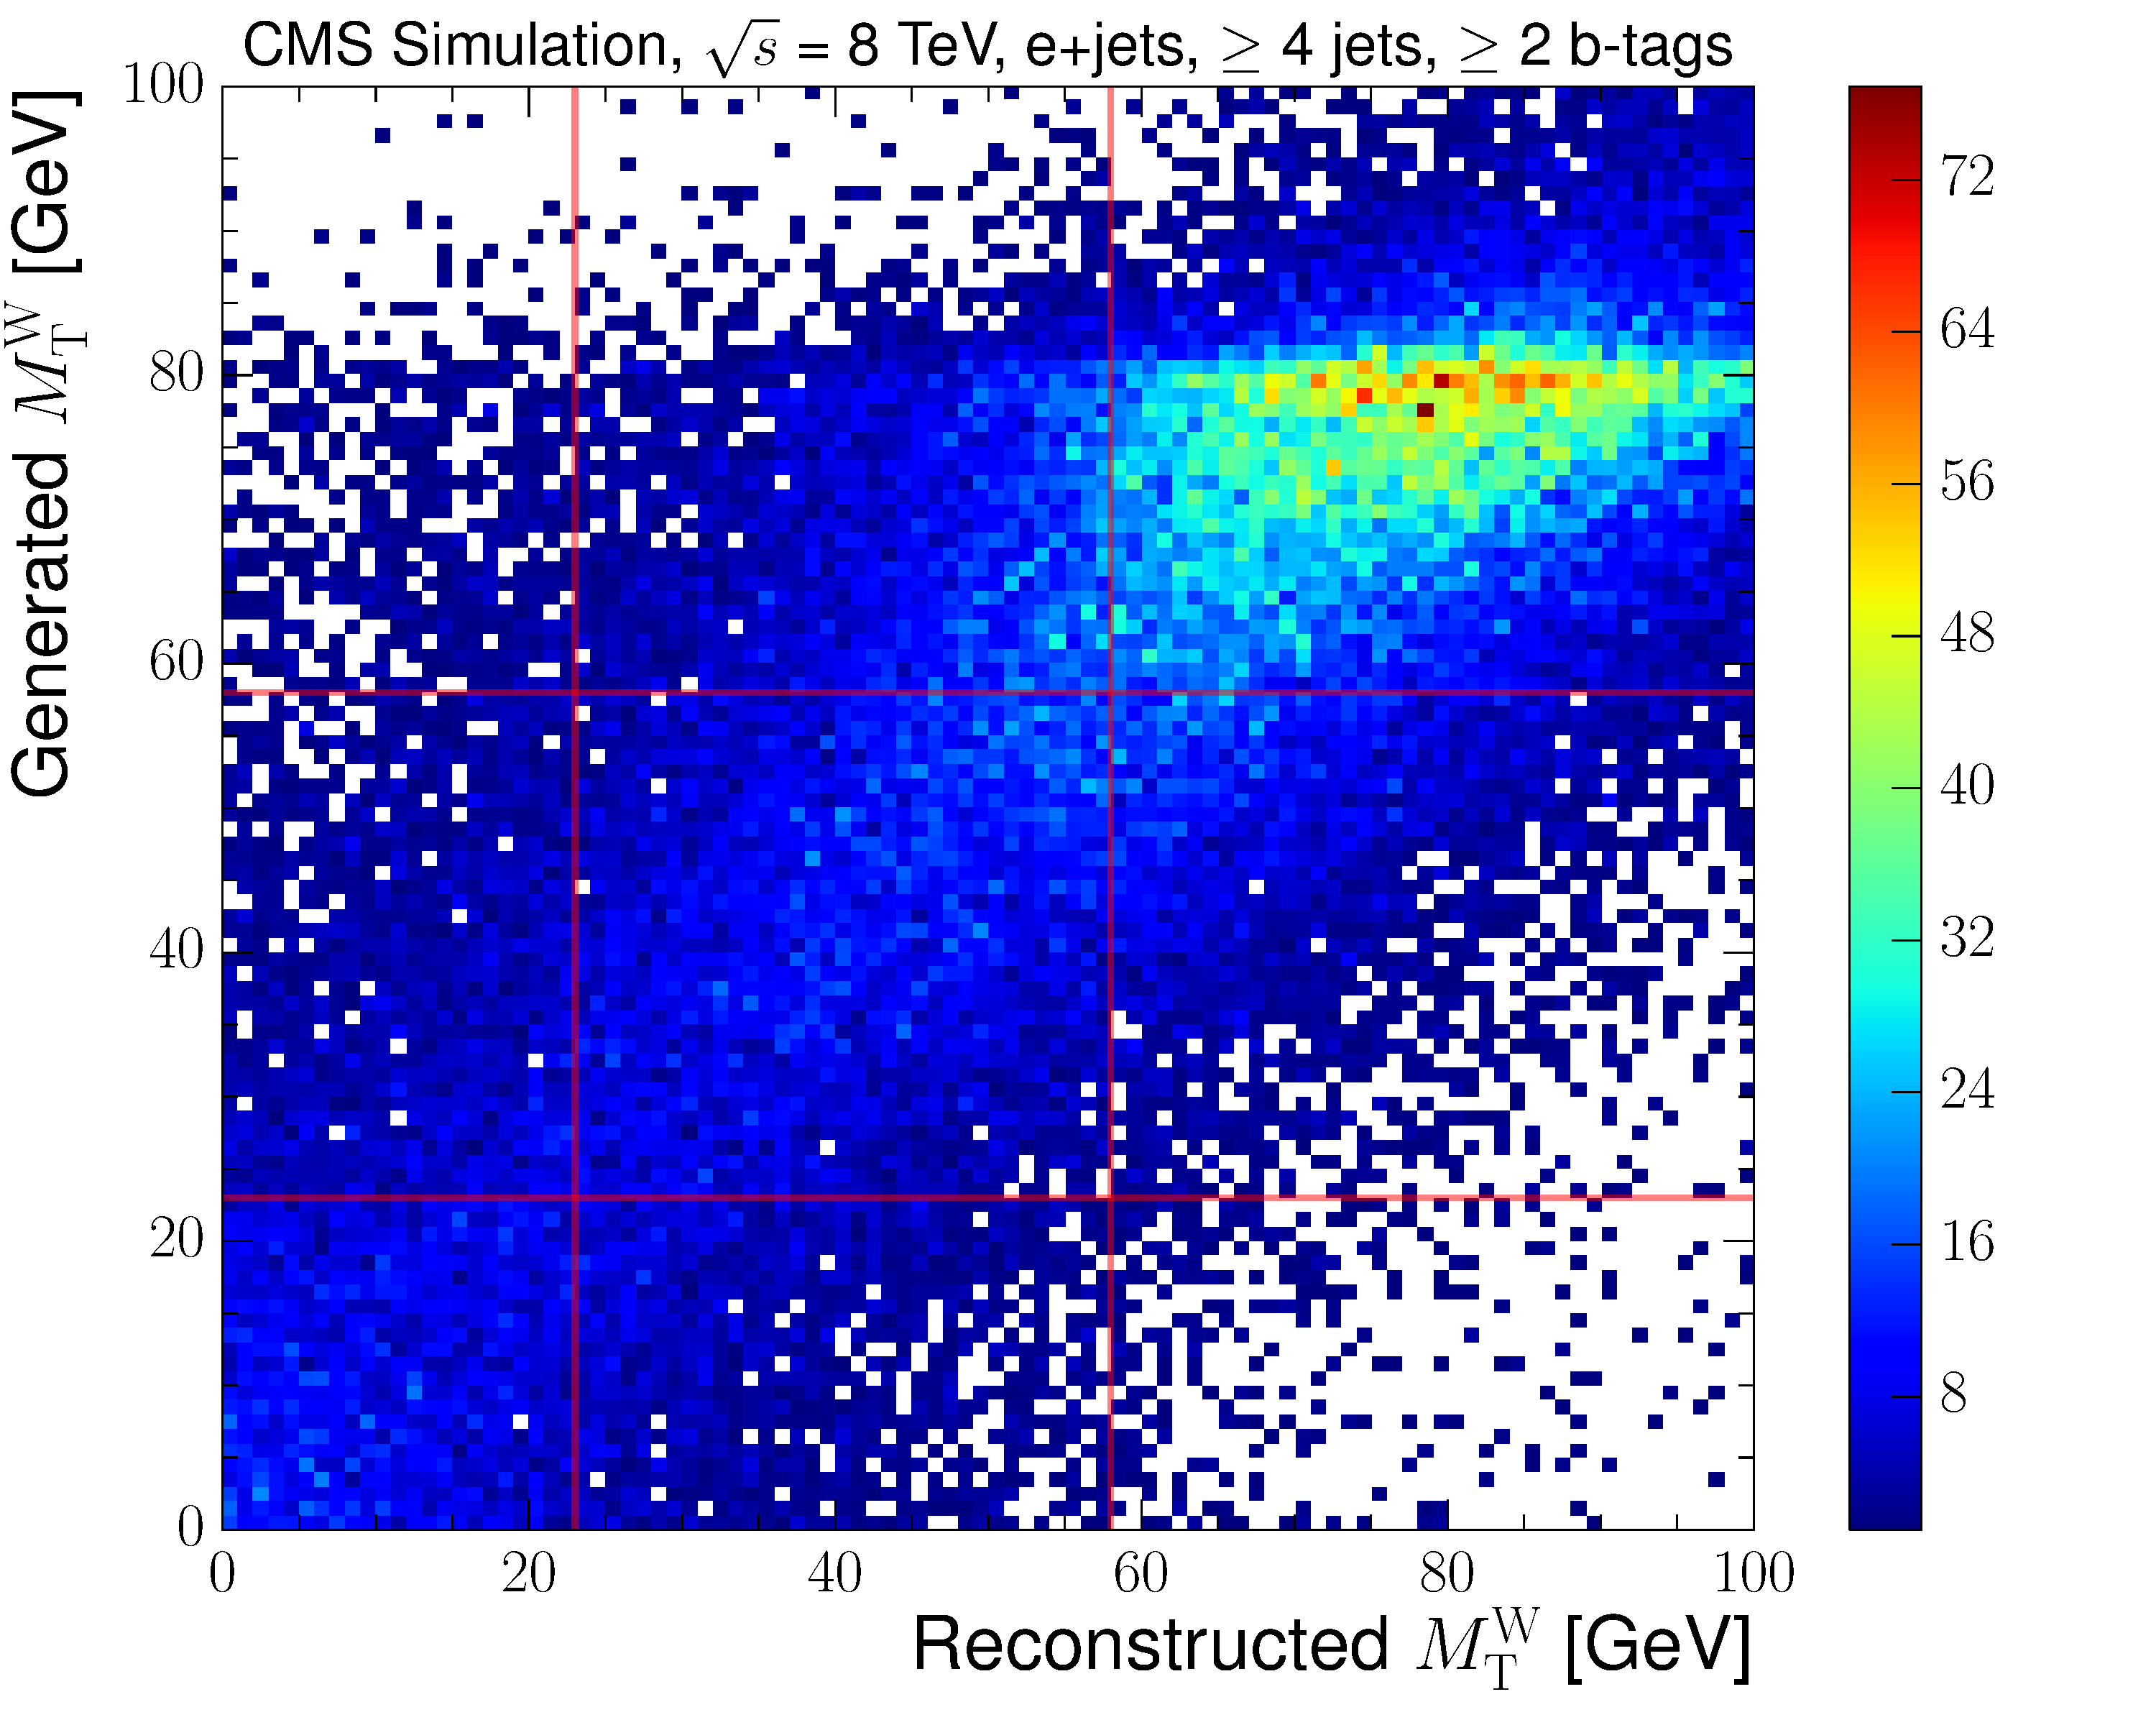
\includegraphics[width=0.48\textwidth]{Chapters/04_Analysis/04b_XSections/images/binning/electron_MT_8TeV.pdf}\\
	 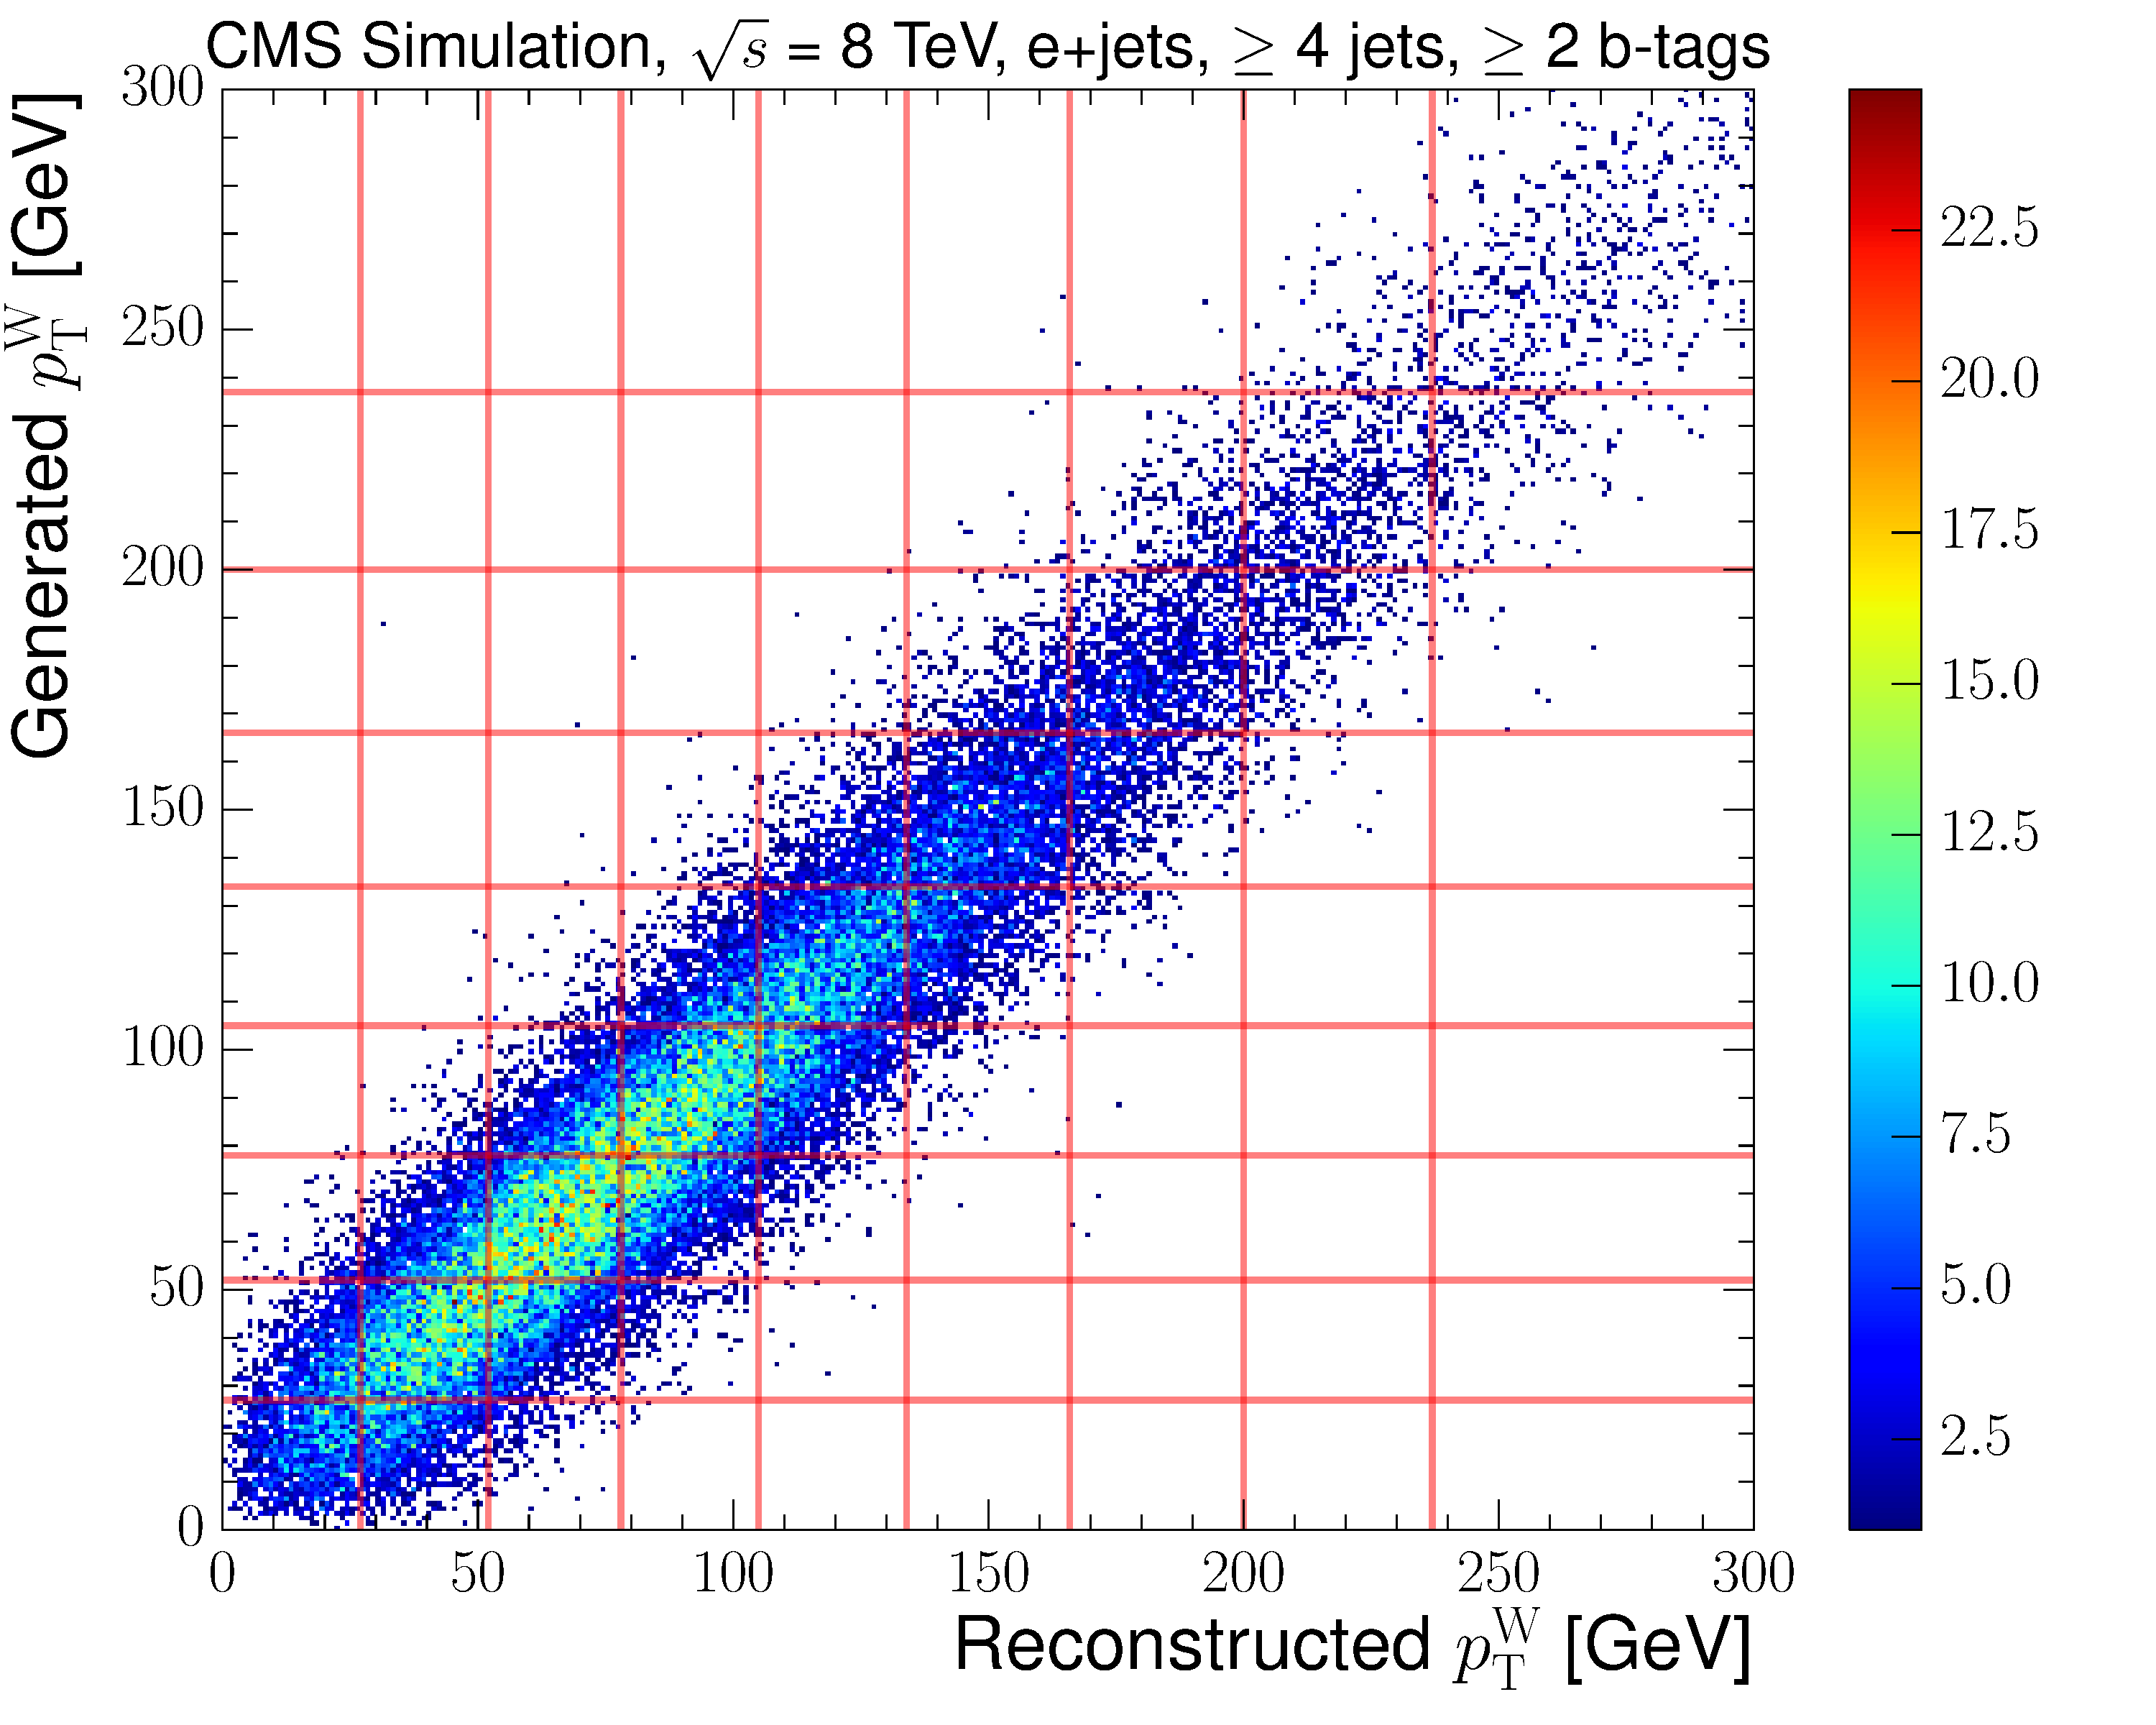
\includegraphics[width=0.48\textwidth]{Chapters/04_Analysis/04b_XSections/images/binning/electron_WPT_8TeV.pdf}\hfill
	 \caption[Generated versus reconstructed distributions of the primary variables at $\roots=8\TeV$.]{Generated
	 versus reconstructed distributions of the primary variables \met (upper left), \HT (upper right), \st
	 (middle left), \mt (middle right) and \wpt (lower) with horizontal and vertical lines representing the
	 boundaries of the selected bins at $\roots=8\TeV$ in the electron+ jets channel. These distributions are
	 obtained using \ttbar simulation.}
     \label{fig:binning_8TeV_electron}
 \end{figure}
\FloatBarrier

\section{Maximum Likelihood Fit}
\label{s:maximum_likelihood_fit}
A maximum log likelihood fit of four templates to data in each bin of the primary variables is used to obtain
the number of events from each process in each bin. Three fitting variables are used because no individual
variable is able to distinguish between all four templates used in the fit:

\begin{itemize}
  \item {\ttbar}
  \item{single-top}
  \item{V+jets (W+jets + Z+jets)}
  \item{QCD multi-jet} 
\end{itemize}

The template distributions are obtained from the following three variables: the absolute pseudorapidity of the
lepton (\abseta), the three-dimensional angle between the lepton and the nearest \bjet ($\alpha$), and the
invariant mass of the three jets with the highest \pt sum ($M3$).

The fit is carried out by maximising the log of the likelihood function (LL):

\begin{equation}
\label{log_likelihood}
LL\left(x_i, d_i\right) = -2 \log{\prod\limits_{i}\frac{x_i^{d_i}\cdot
e^{-x_i}}{d_i!}}=-2\sum\limits_{i}\log{\left(\frac{x_i^{d_i}\cdot e^{-x_i}}{d_i!}\right)}.
\end{equation}

where $i$ is the bin index in the template, $x_i$ is the total of all the templates in bin $i$, and $d_i$ is
the observed number of data events in  bin $i$. $x_i$ is defined to be

\begin{equation}
\label{eq:sum_mc}
x_i = \sum\limits_{j}N_{j}x_{i\,j},\;\text{with}\;\sum\limits_{i}x_{i\,j}=1\ \text{for each process}.
\end{equation}

where $x_{i\,j}$ represents the templates and $N_{j}$ represents the normalisations of the templates \ie the
fit parameters. Fitting using more than one fitting variable (the three aforementioned fitting variables), the
log likelihoods are summed:
\begin{equation}
\label{eq:log_L_final}
LL\left(x, d\right) = -\frac{2}{n} \sum\limits_{k=1,n} \log{L_k}
\end{equation}

where $L_k$ is the likelihood function of each of the different fit variables. Here the division by $n$
accounts for the fact that the same information is used in all three fit variables, and so full correlation is
assumed between the three fitting variables, which provides a conservative estimate of the uncertainties in
the resulting fitted parameters. The fit operates by adjusting the normalisation of each template with the aim
of equating $x_{i}$ and $d_{i}$ in each bin of each template. The starting normalisations in the templates are
obtained from simulation after the full selection has been applied (this includes the QCD template, although
the shape for this is obtained from data).

\subsection{Choice of templates}
\label{choice_of_templates}

\ttbar, single-top and V+jets templates are taken from simulation, while the QCD template is extracted from
data as described in Section~\ref{ss:background_selection}. The W+jets and Z+jets templates are combined
firstly due to the similar shapes of the distributions in these two background processes, and secondly due to
limited statistics available in simulation. The four template shapes in each of the three fitting variables at
$\roots=7\TeV$ in both channels are shown in Figure~\ref{fig:fit_variable_distributions_7TeV}. The
corresponding plots for $\roots=8\TeV$ are shown in Appendix~\ref{as:fitting_variables_distributions}.

This combination of fitting variables was selected because they are only weakly correlated to the primary
variables under investigation, and they show good discrimination between the four templates.
Single top events have similar signatures to \ttbar events, with a central lepton from the decay of the single
top, leading to a single top template that is similar to the \ttbar template in the electron \abseta and muon
\abseta distributions. In the $\alpha$ distribution, the similarity is attributable to the fact that the
closest \bjet from the lepton is generally a \bjet from the decay of a \tquark. However, the average boost for
single top events is lower than in \ttbar events, leading to a wider single top template.
The M3 variable will be a combination of the jets from the hadronically decaying \tquark (a \bjet and two
other jets from the \W-boson, which may include a second \bjet) in \ttbar events, whereas in the other
templates, M3 will simply correspond to some random combination of jets in the event. Hence, M3 shows the best discrimination between the single top
and \ttbar templates.

\begin{figure}[hbtp]
    \centering
     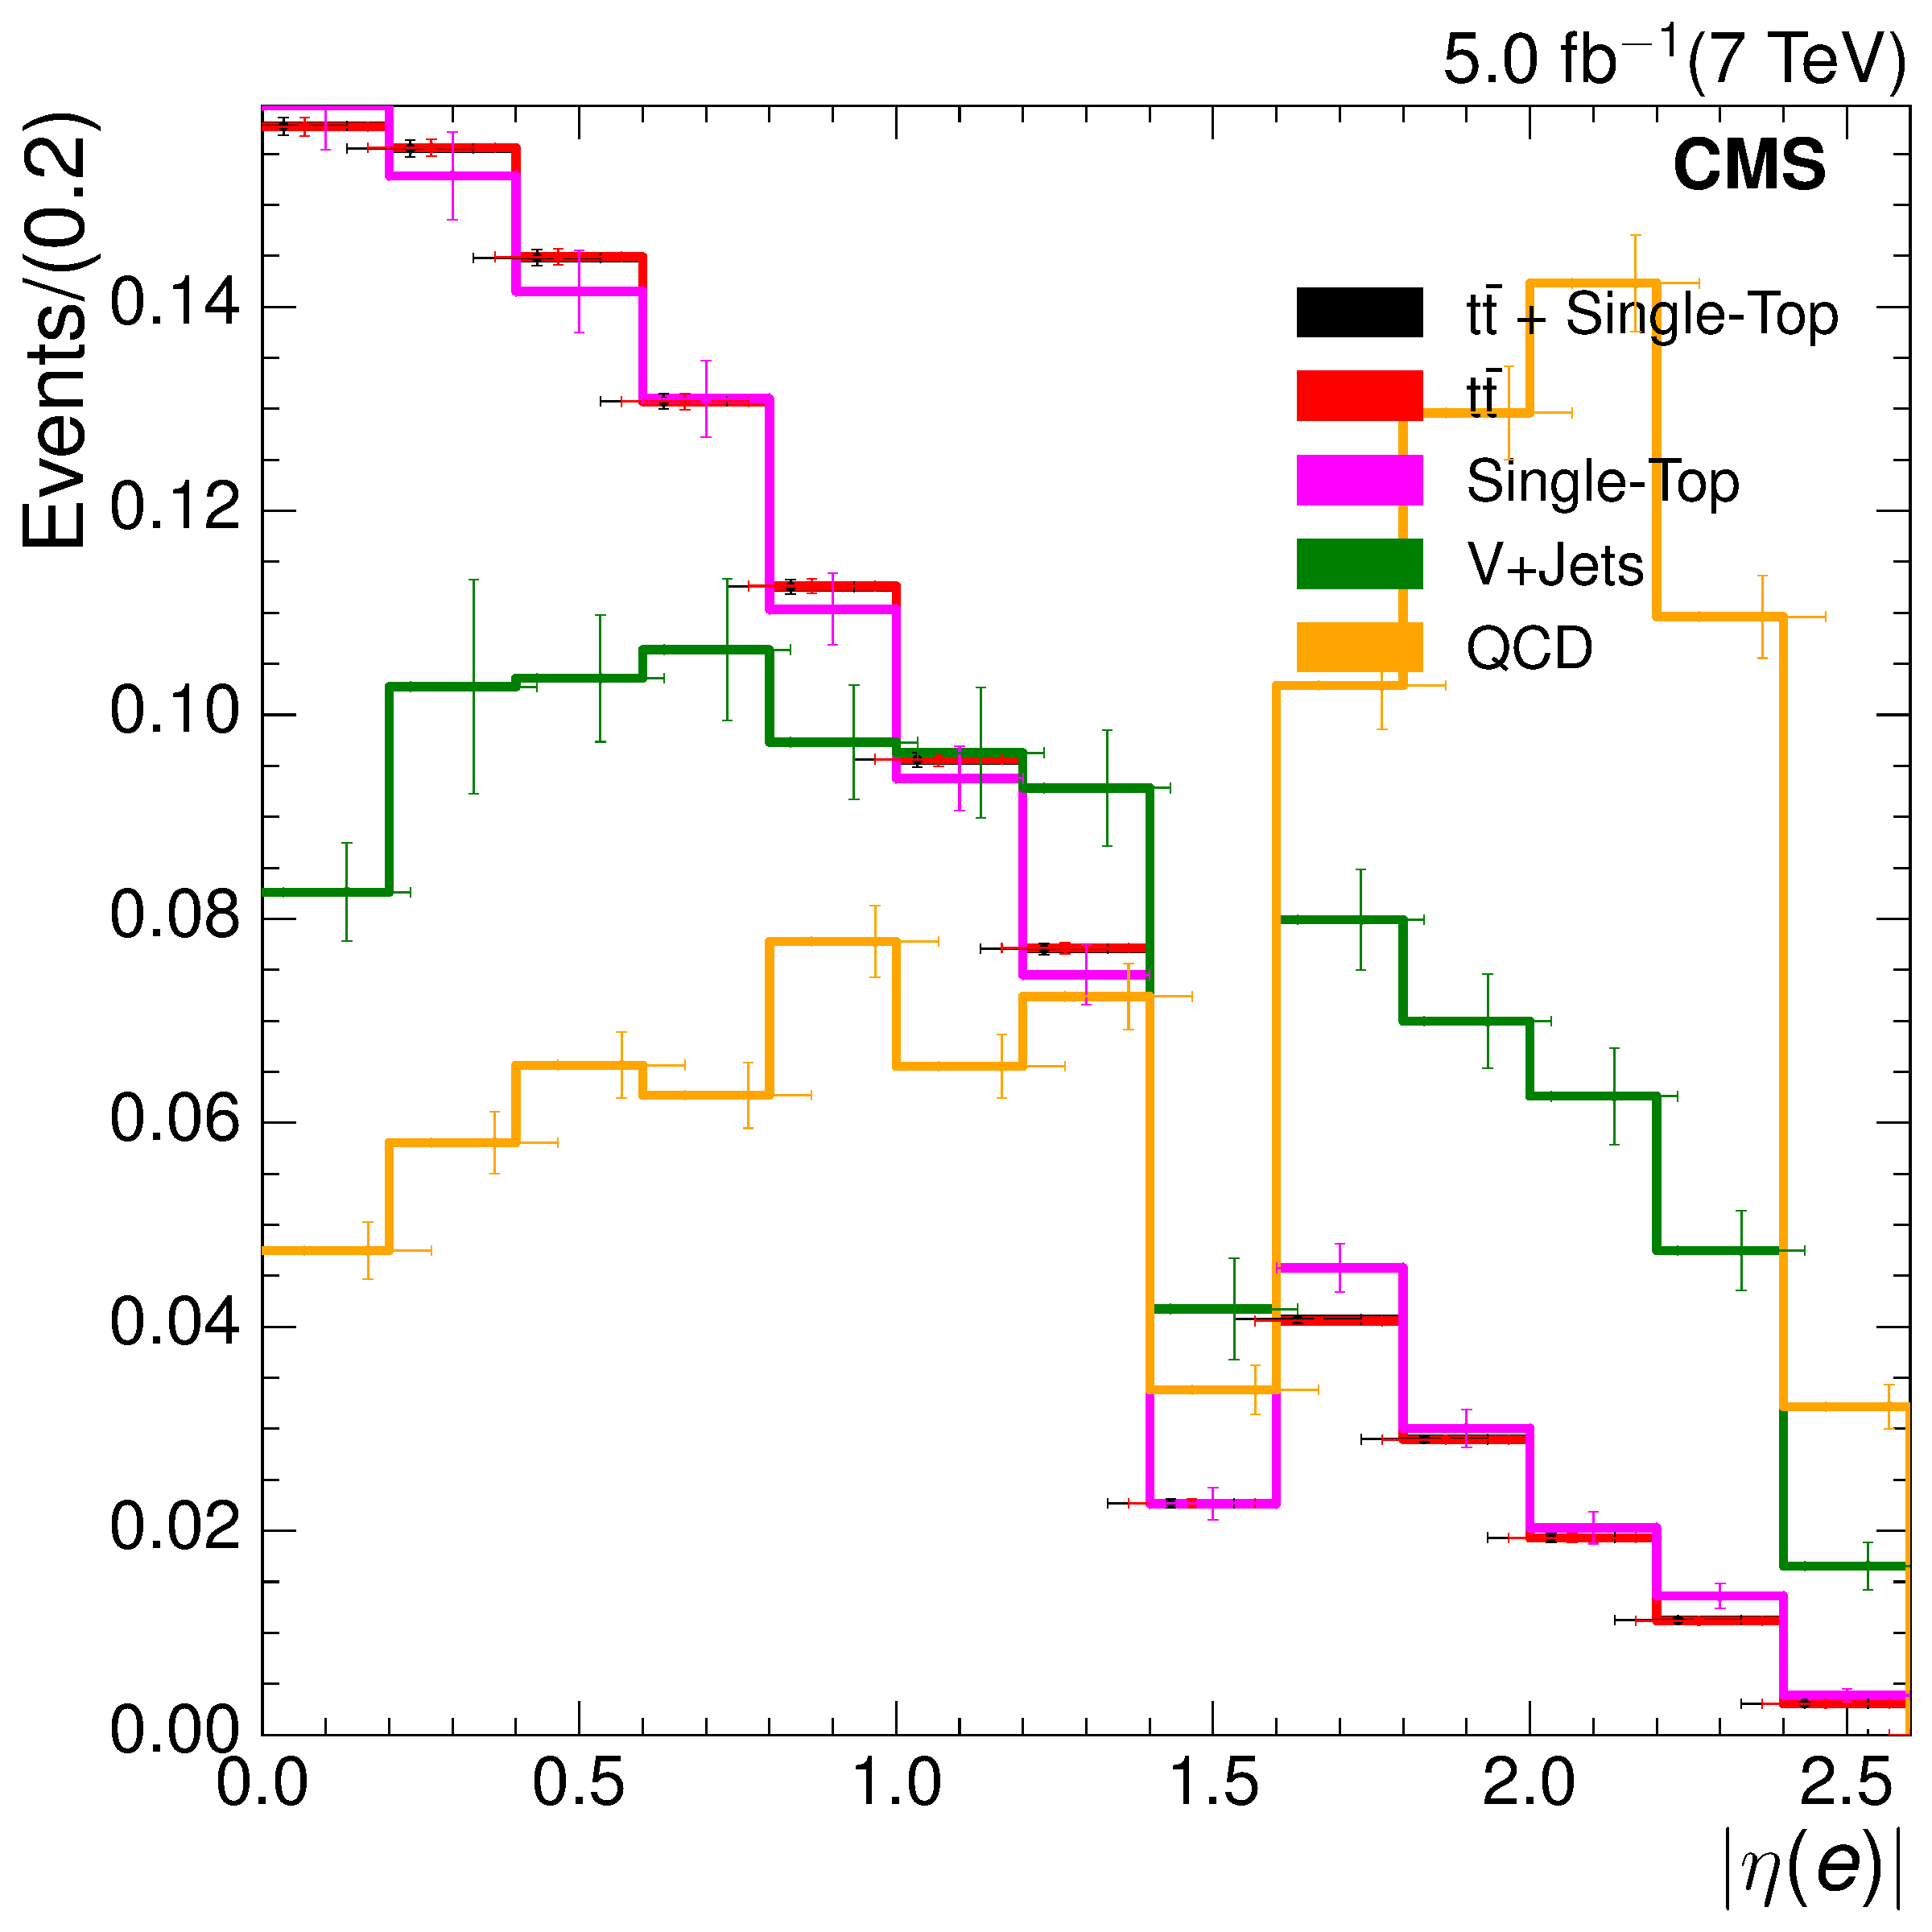
\includegraphics[width=0.48\textwidth]{Chapters/04_Analysis/04b_XSections/images/7TeV/fit_variables/electron/MET/electron_absolute_eta/MET_inclusive_electron_absolute_eta_2orMoreBtags_templates.pdf}\hfill
     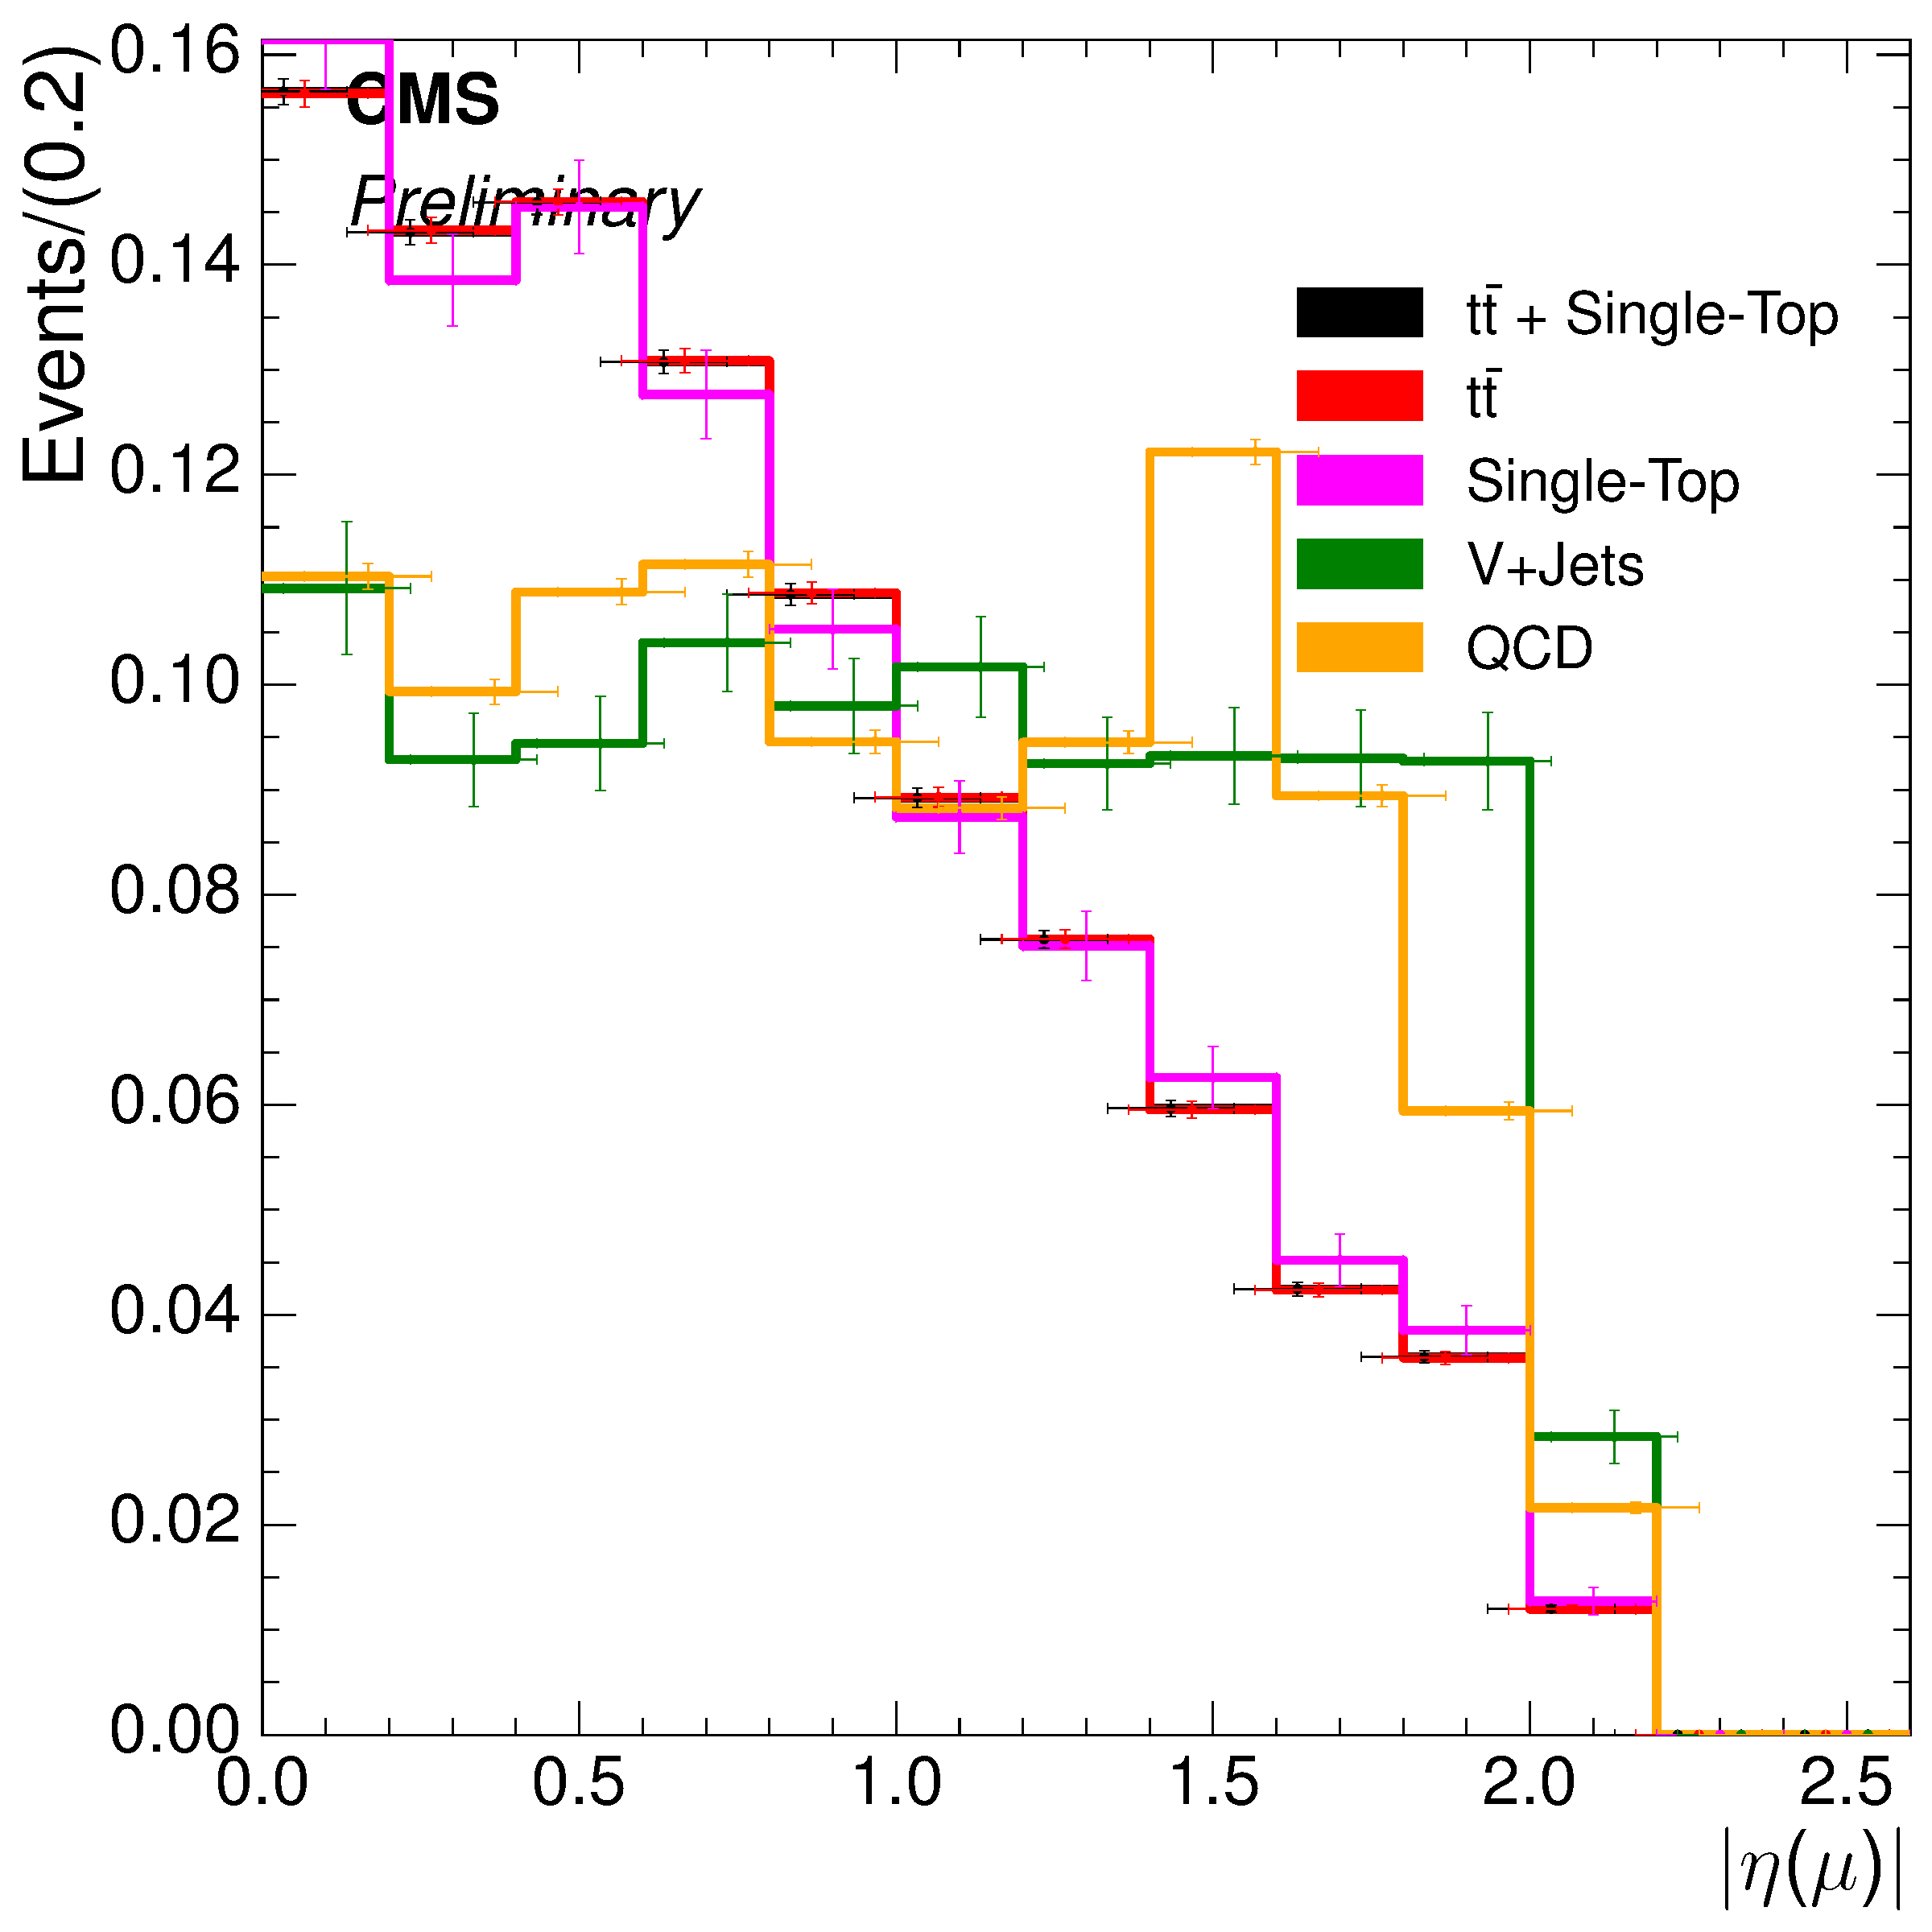
\includegraphics[width=0.48\textwidth]{Chapters/04_Analysis/04b_XSections/images/7TeV/fit_variables/muon/MET/muon_absolute_eta/MET_inclusive_muon_absolute_eta_2orMoreBtags_templates.pdf}\\
     \includegraphics[width=0.48\textwidth]{Chapters/04_Analysis/04b_XSections/images/7TeV/fit_variables/electron/MET/angle_bl/MET_inclusive_angle_bl_2orMoreBtags_templates.pdf}\hfill
     \includegraphics[width=0.48\textwidth]{Chapters/04_Analysis/04b_XSections/images/7TeV/fit_variables/muon/MET/angle_bl/MET_inclusive_angle_bl_2orMoreBtags_templates.pdf}\\
     \includegraphics[width=0.48\textwidth]{Chapters/04_Analysis/04b_XSections/images/7TeV/fit_variables/electron/MET/M3/MET_inclusive_M3_2orMoreBtags_templates.pdf}\hfill
     \includegraphics[width=0.48\textwidth]{Chapters/04_Analysis/04b_XSections/images/7TeV/fit_variables/muon/MET/M3/MET_inclusive_M3_2orMoreBtags_templates.pdf}\\
	 \caption[Normalised distributions of the templates for the three fit variables, inclusive across all primary
	 variable bins at $\roots=7\TeV$.]{Normalised distributions of the templates for the three fit variables
	 lepton \abseta (upper), $\alpha$ (middle) and M3 (lower) inclusive across all primary variable bins at
	 $\roots=7\TeV$ in the electron+jets channel (left) and in the muon+jets channel (right).}
     \label{fig:fit_variable_distributions_7TeV}
\end{figure}

\FloatBarrier

The QCD templates, in particular those in higher bins of the primary variables, contain lower statistics than
those in lower bins. Therefore, the inclusive QCD template shape, \ie the QCD distribution over all bins, is
used for the fitting process in every bin. Figure~\ref{fig:fit_variable_qcd_comparisons_8TeV} shows a
comparison between QCD templates at $\roots=8\TeV$ in the lowest three bins of the \met variable and also the
inclusive \met QCD template. It can be seen that the third \met bin already shows large statistical errors due
to low numbers of events, and that the inclusive template is largely shaped by events in the first two bins.
Therefore, the inclusive QCD template is used rather than those in individual bins. %Similar plots showing the
%same behaviour for the other primary variables at $\roots=8\TeV$ are shown in
%Appendix~\ref{as:fitting_variable_QCD_template_comparisons}.

\begin{figure}[hbtp]
    \centering
     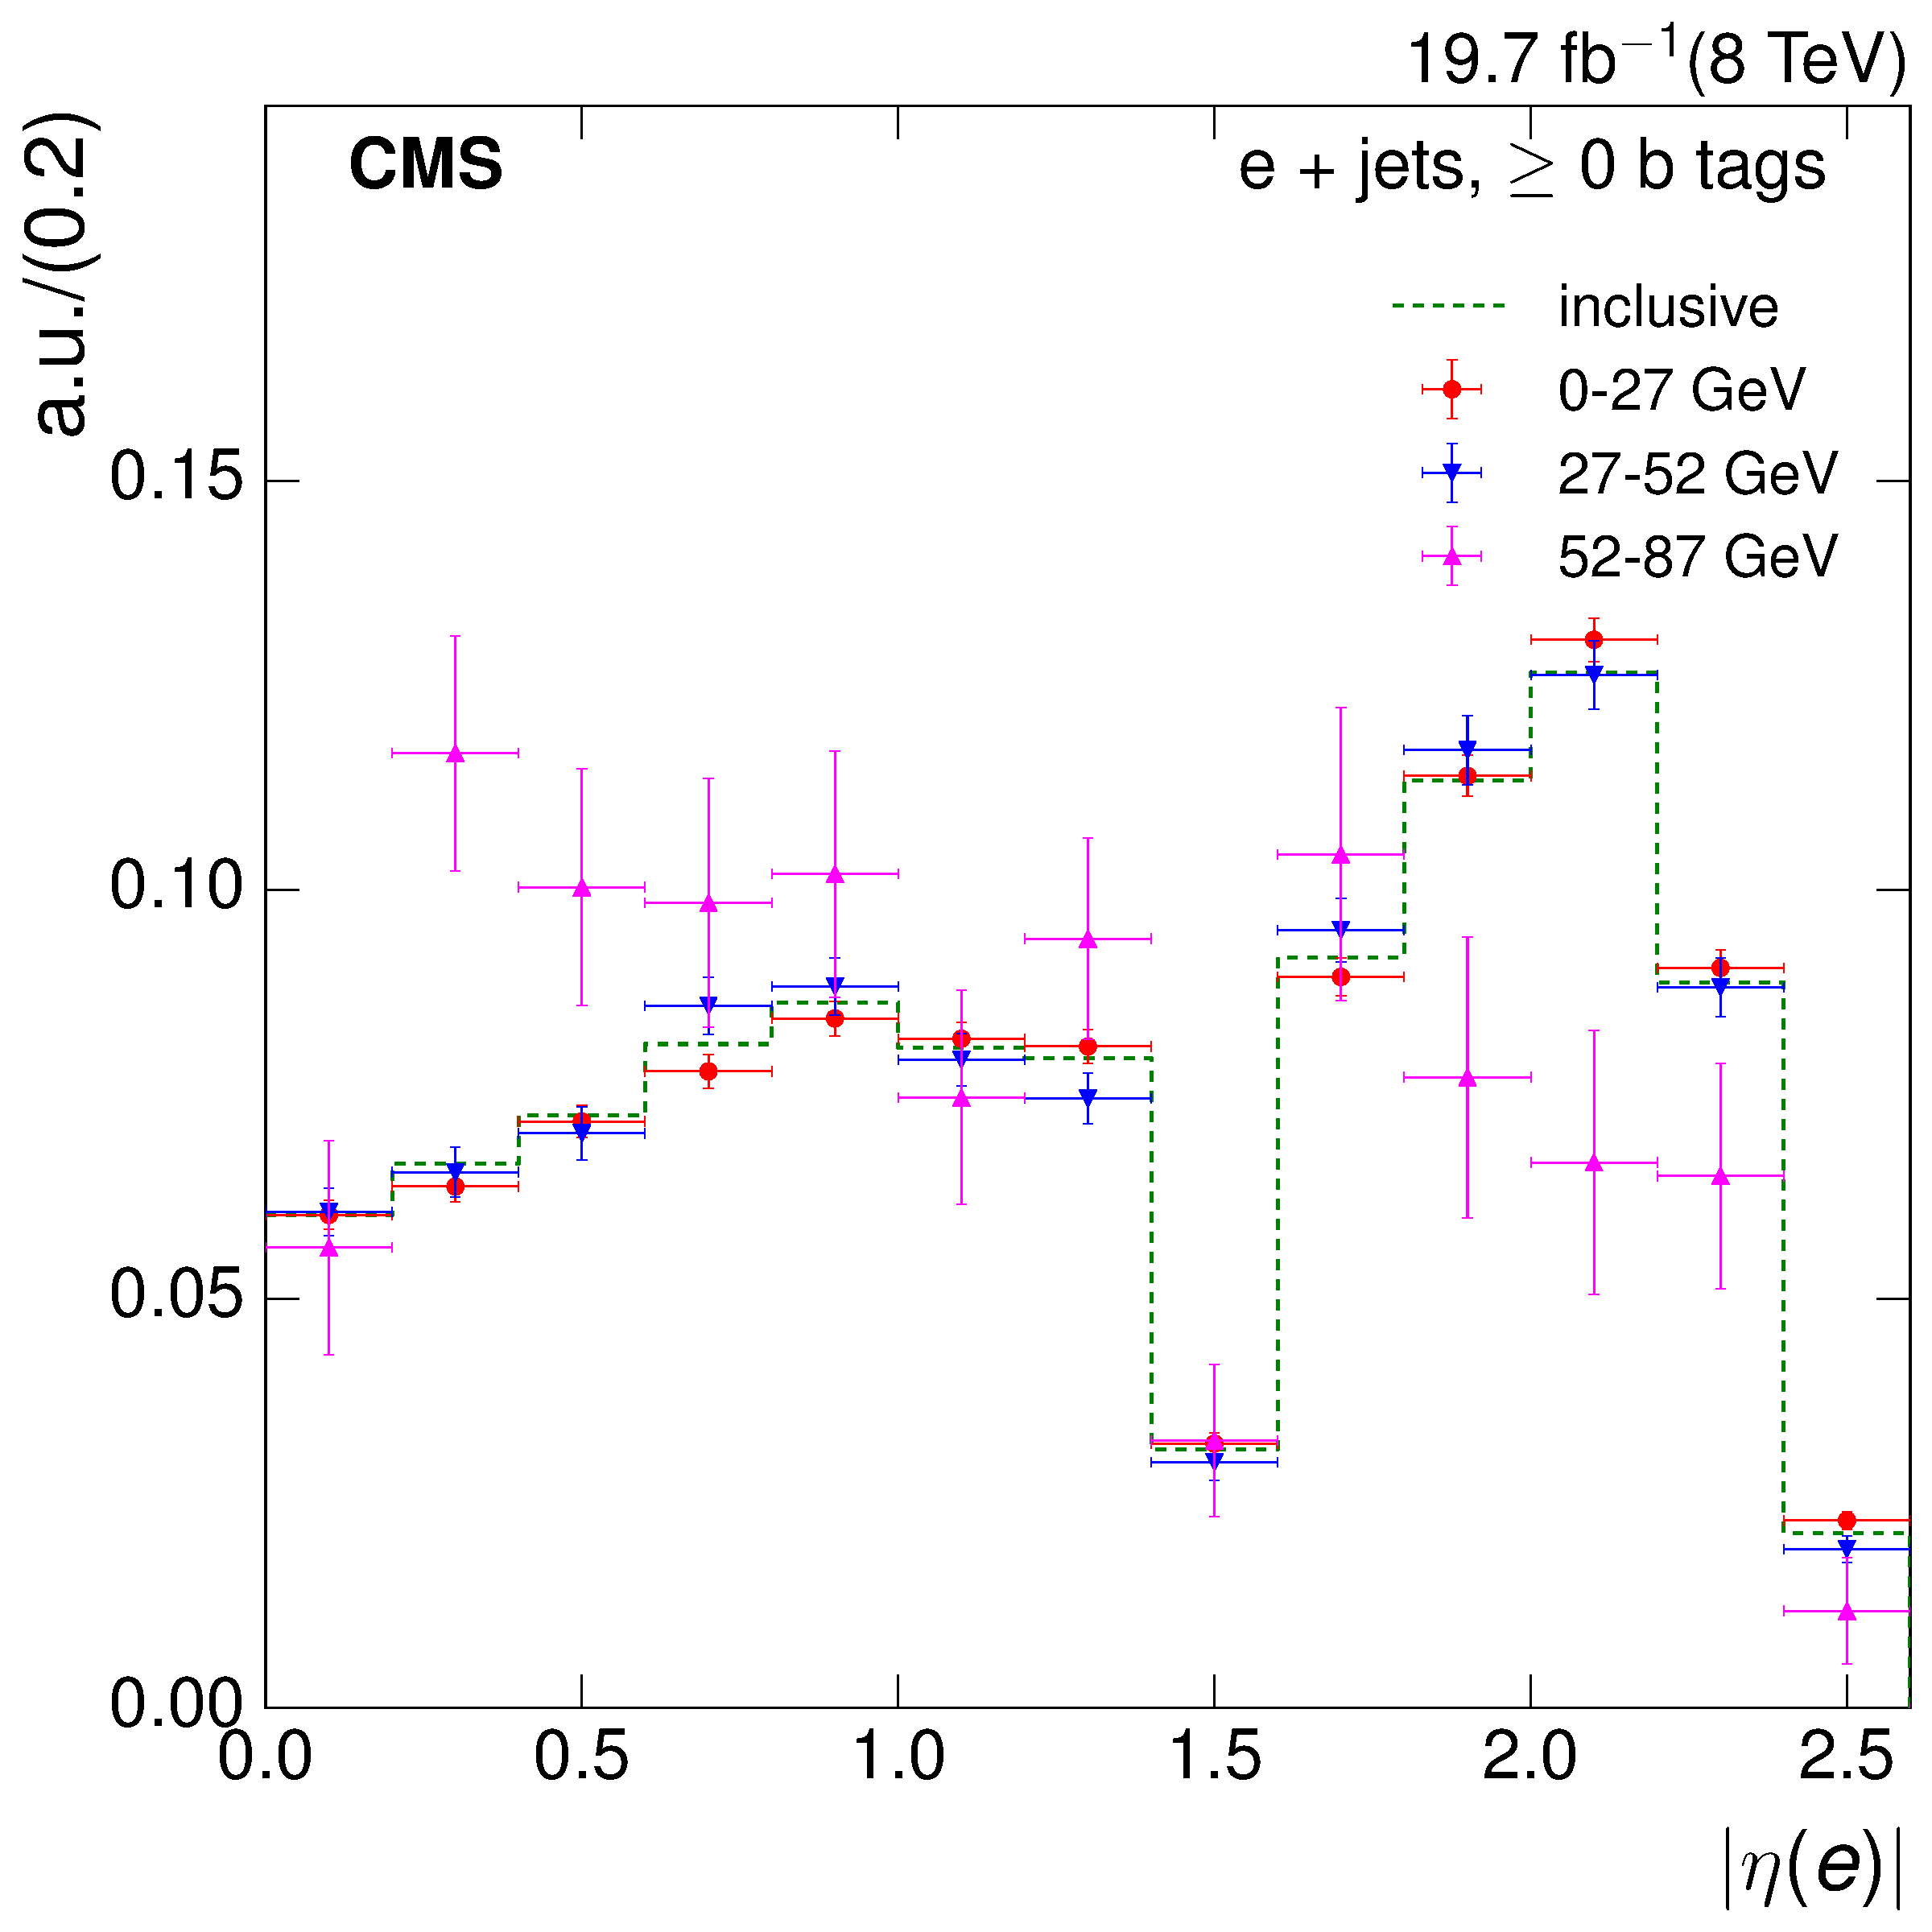
\includegraphics[width=0.48\textwidth]{Chapters/04_Analysis/04b_XSections/images/8TeV/fit_variables/electron/MET/electron_absolute_eta/qcd/MET_electron_absolute_eta_0orMoreBtag_QCD_template_comparison.pdf}\hfill
     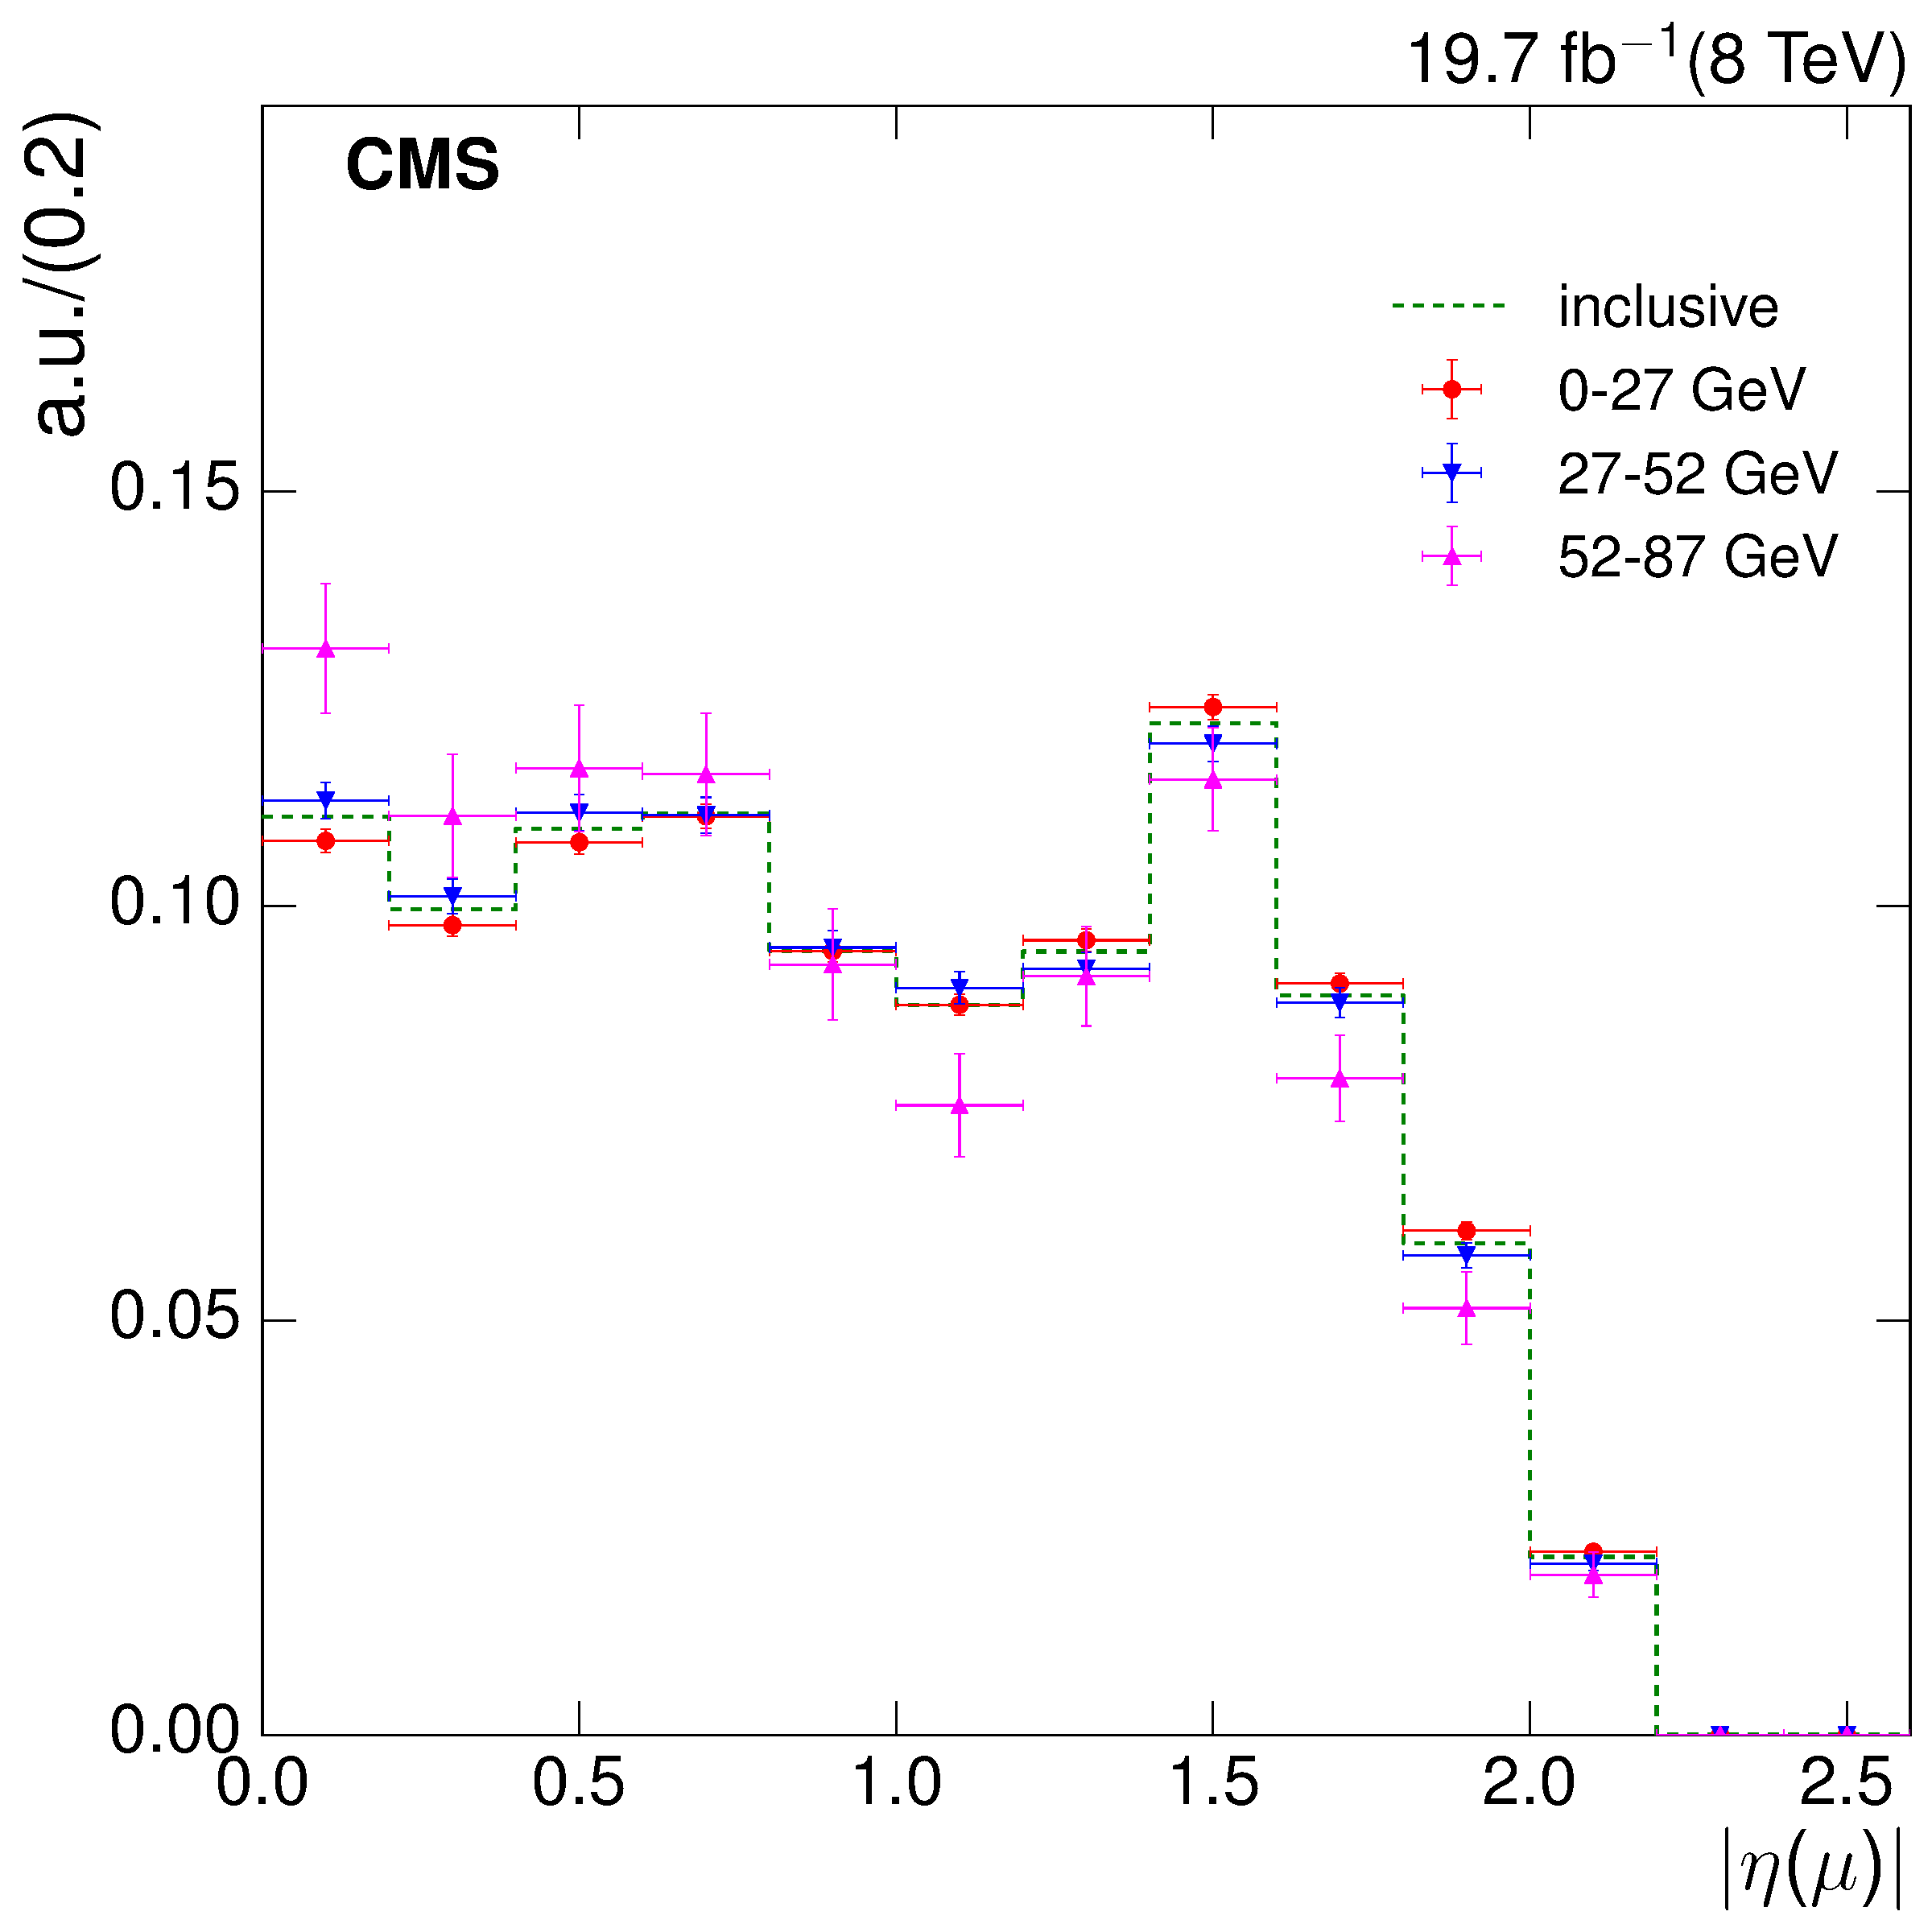
\includegraphics[width=0.48\textwidth]{Chapters/04_Analysis/04b_XSections/images/8TeV/fit_variables/muon/MET/muon_absolute_eta/qcd/MET_muon_absolute_eta_0orMoreBtag_QCD_template_comparison.pdf}\\
     \includegraphics[width=0.48\textwidth]{Chapters/04_Analysis/04b_XSections/images/8TeV/fit_variables/electron/MET/angle_bl/qcd/MET_angle_bl_1orMoreBtag_QCD_template_comparison.pdf}\hfill
     \includegraphics[width=0.48\textwidth]{Chapters/04_Analysis/04b_XSections/images/8TeV/fit_variables/muon/MET/angle_bl/qcd/MET_angle_bl_1orMoreBtag_QCD_template_comparison.pdf}\\
     \includegraphics[width=0.48\textwidth]{Chapters/04_Analysis/04b_XSections/images/8TeV/fit_variables/electron/MET/M3/qcd/MET_M3_0orMoreBtag_QCD_template_comparison.pdf}\hfill
     \includegraphics[width=0.48\textwidth]{Chapters/04_Analysis/04b_XSections/images/8TeV/fit_variables/muon/MET/M3/qcd/MET_M3_0orMoreBtag_QCD_template_comparison.pdf}\\
	 \caption[Normalised distributions of the QCD templates for the three fit variables in \met bins
	 at $\roots=8\TeV$.]{Normalised distributions of the QCD templates for the three fit variables lepton \abseta
	 (upper), $\alpha$ (middle) and M3 (lower) inclusive across all \met bins and for the lowest three \met bins
	 at $\roots=8\TeV$ in the electron+jets channel (left) and in the muon+jets channel (right).}
     \label{fig:fit_variable_qcd_comparisons_8TeV}
\end{figure}

An inclusive template is also used in the V+jets (W+jets + Z+jets) template for the same reason.
Figure~\ref{fig:MET_fit_variable_vjets_comparisons_8TeV} shows a comparison between the V+jets templates at
$\roots=8\TeV$ in each \met bin and also the inclusive \met V+jets template.
As is the case for the QCD background template, it can be seen in the V+jets templates that there are
diminished statistics available in higher bins, and the inclusive template shape is largely governed by the
lower bins. %Similar plots demonstrating the same behaviour for the other primary variables at $\roots=8\TeV$
%are shown in Appendix~\ref{as:fitting_variable_vjets_template_comparisons}.

\begin{figure}[hbtp]
    \centering
     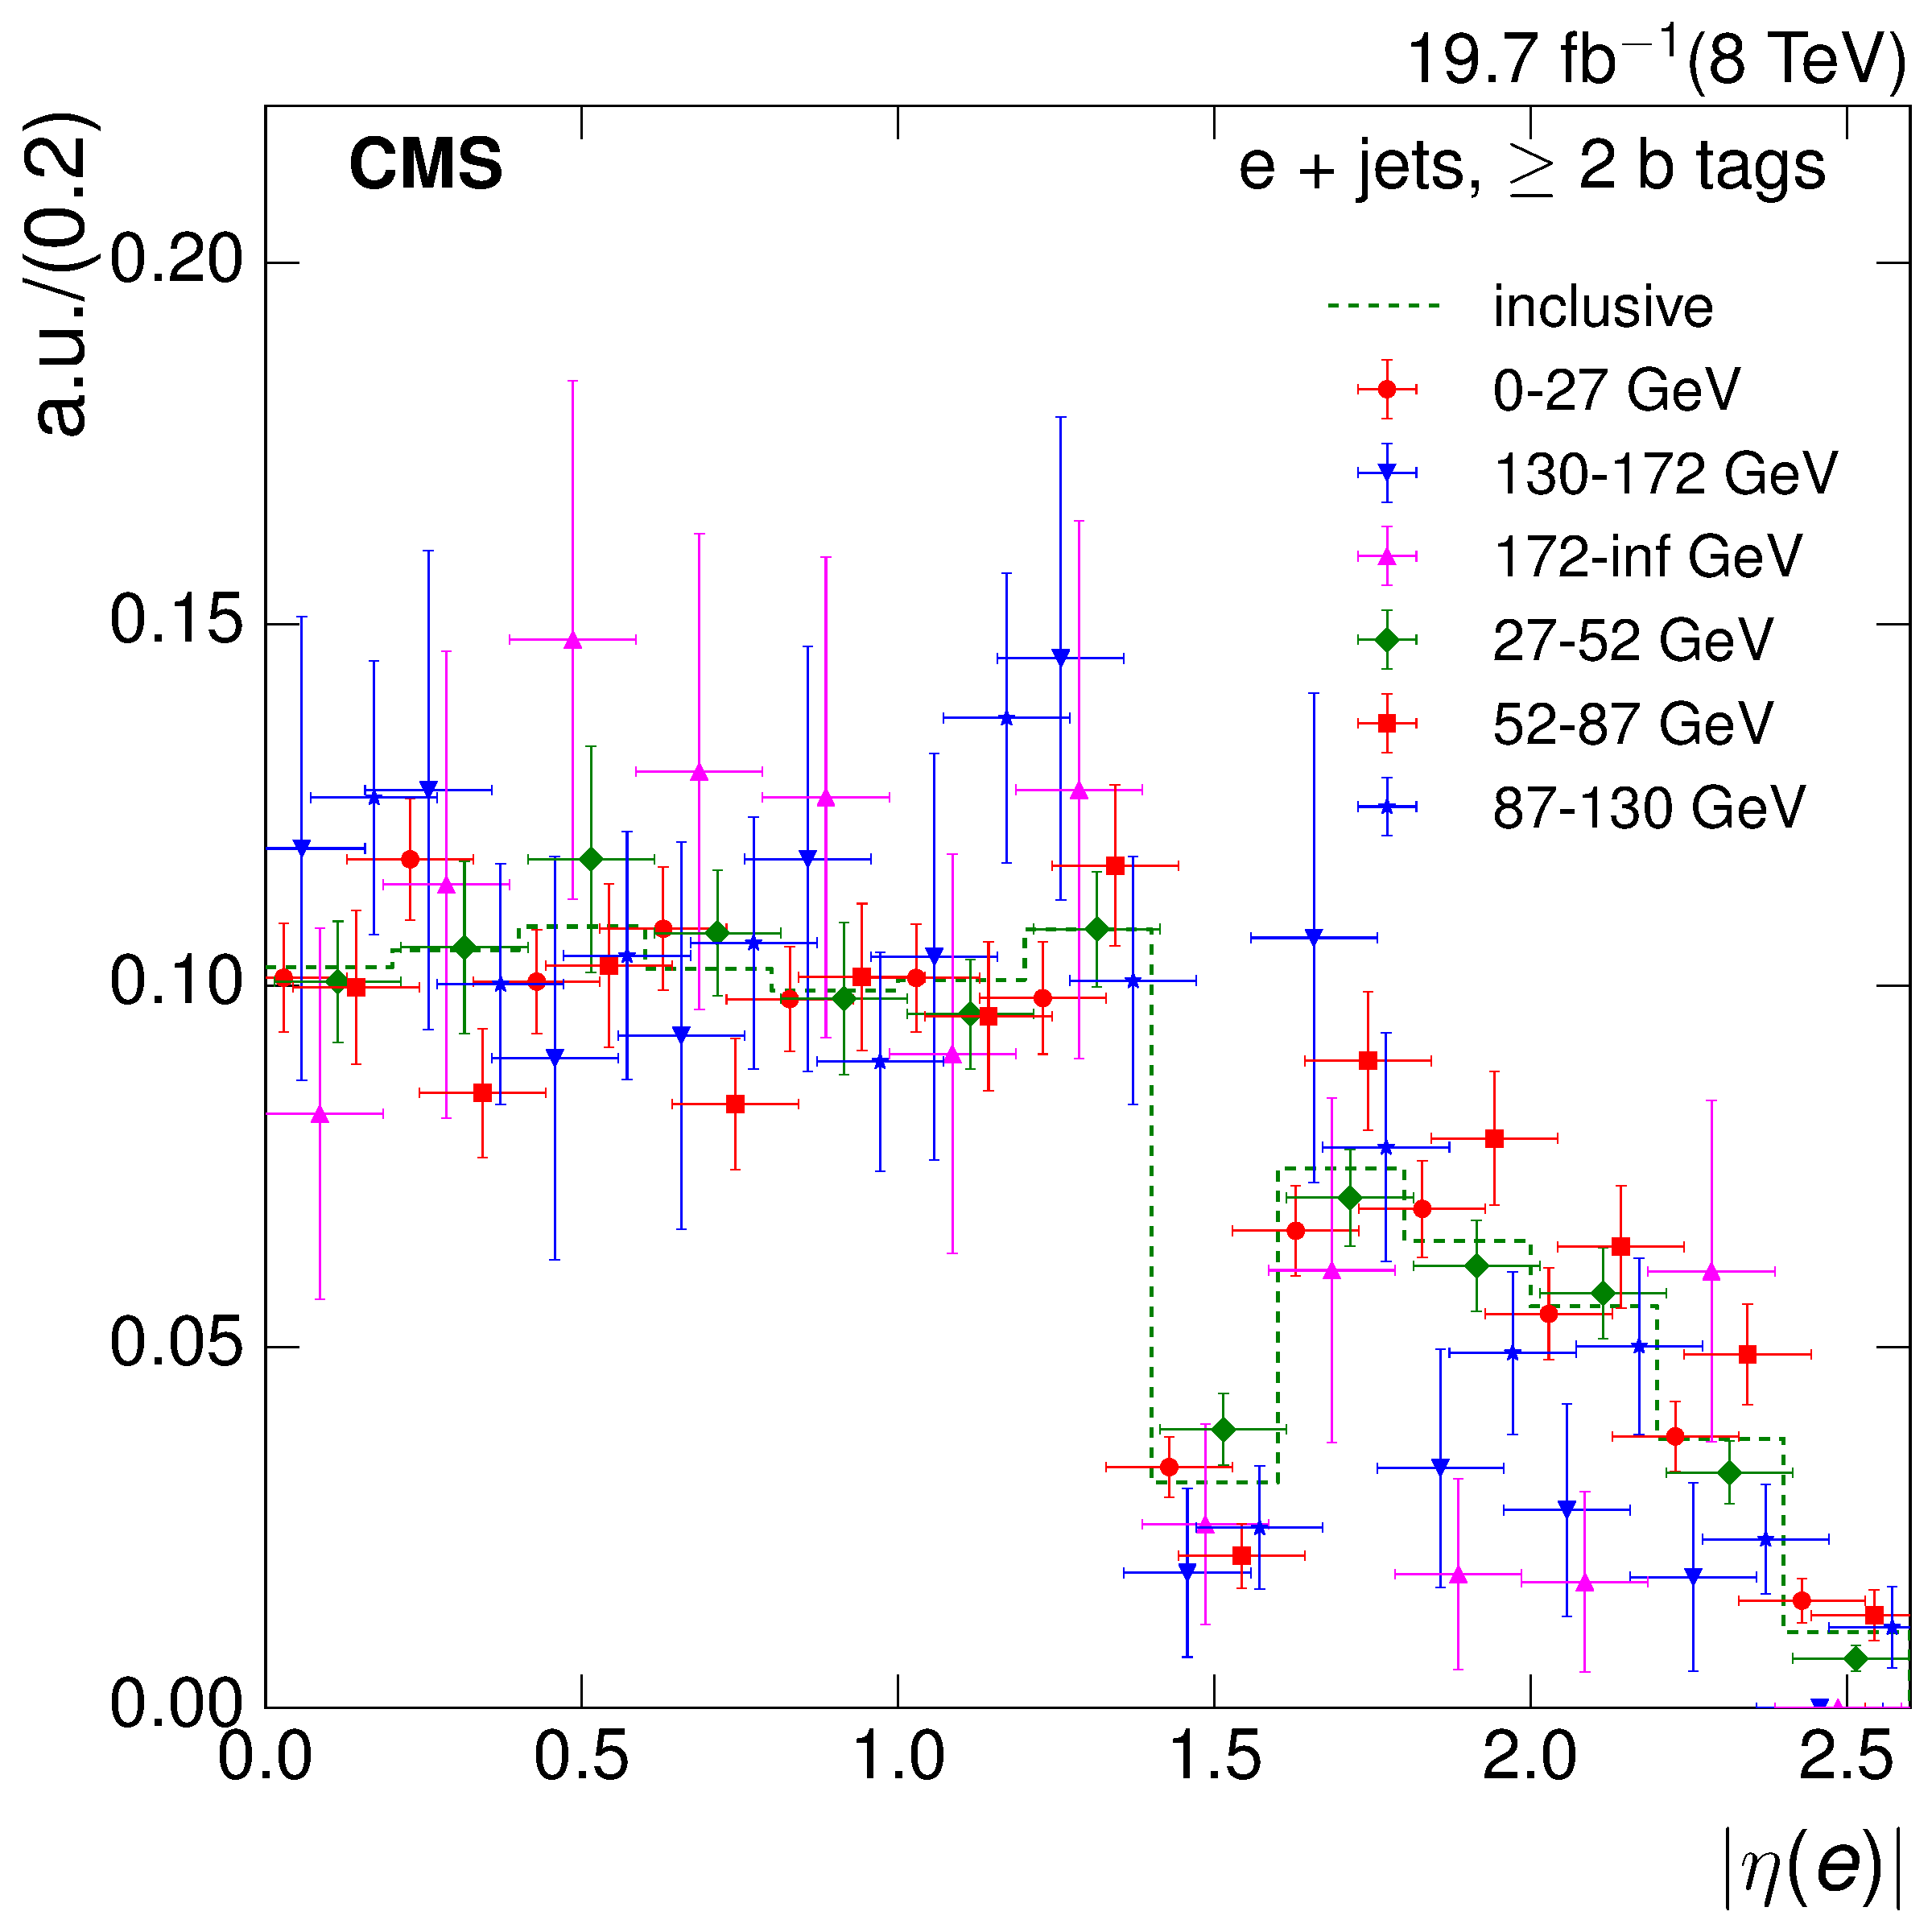
\includegraphics[width=0.48\textwidth]{Chapters/04_Analysis/04b_XSections/images/8TeV/fit_variables/electron/MET/electron_absolute_eta/vjets/MET_electron_absolute_eta_2orMoreBtags_VJets_template_comparison.pdf}\hfill
     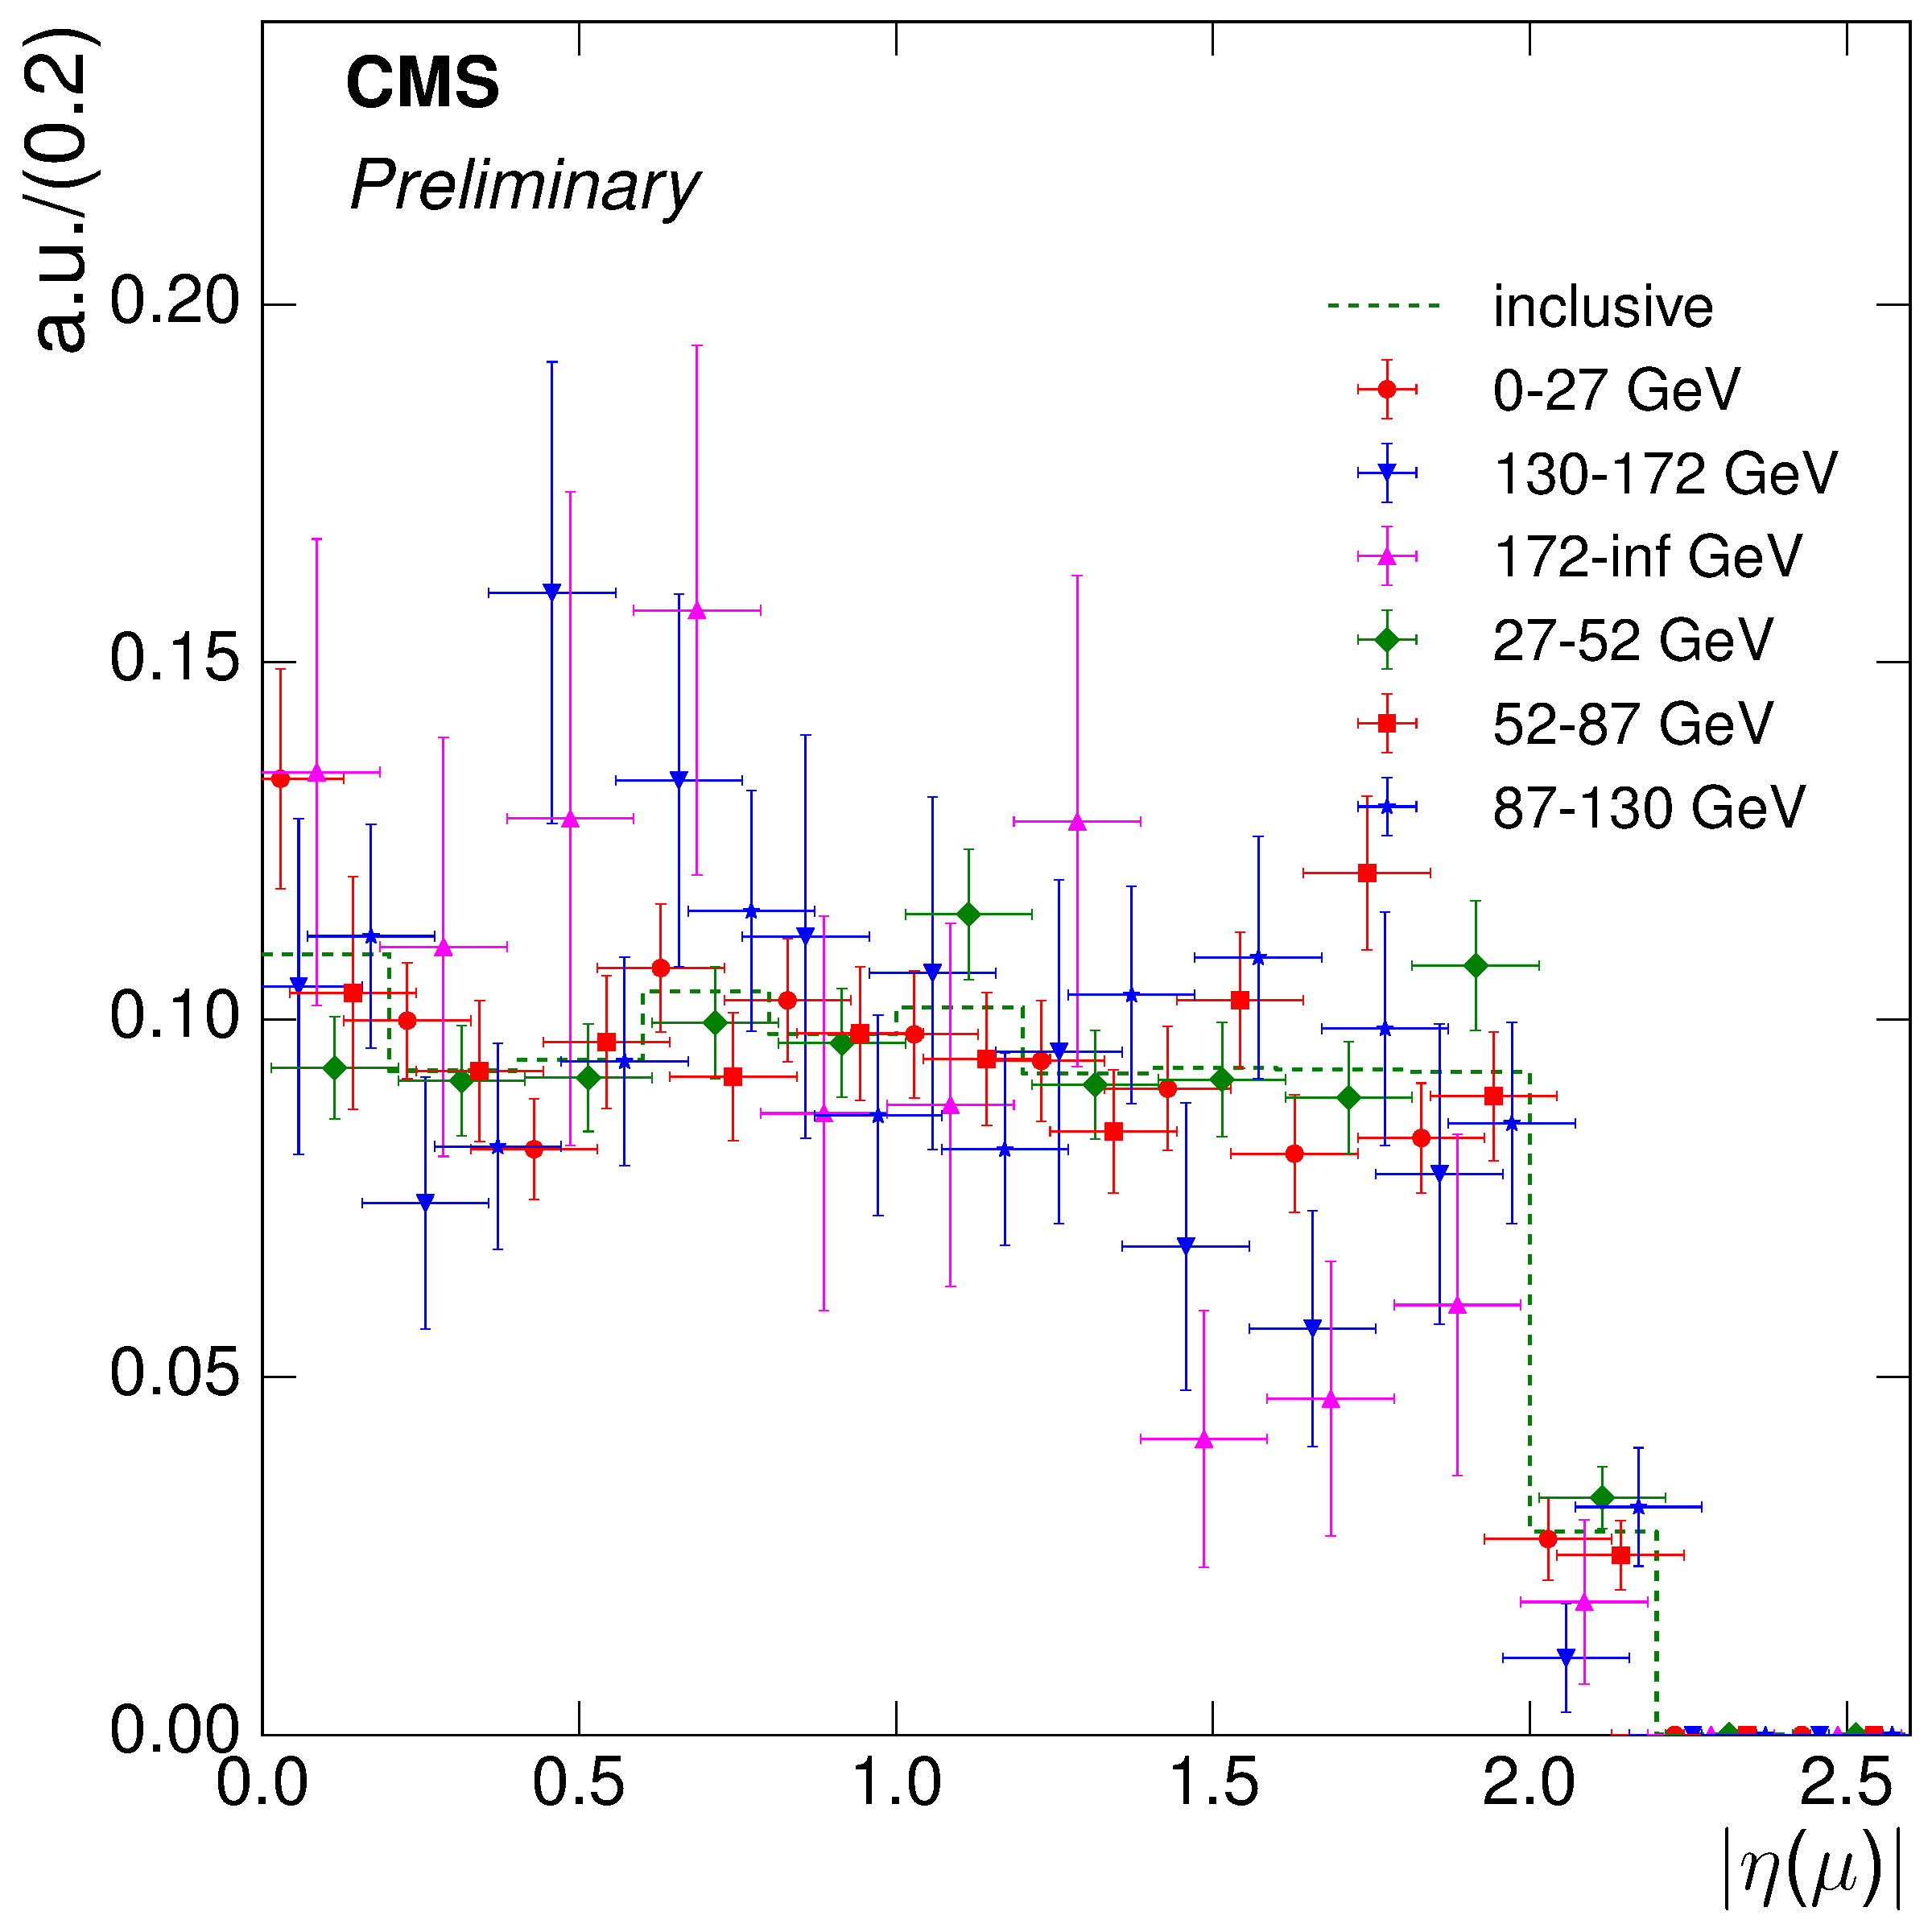
\includegraphics[width=0.48\textwidth]{Chapters/04_Analysis/04b_XSections/images/8TeV/fit_variables/muon/MET/muon_absolute_eta/vjets/MET_muon_absolute_eta_2orMoreBtags_VJets_template_comparison.pdf}\\
     \includegraphics[width=0.48\textwidth]{Chapters/04_Analysis/04b_XSections/images/8TeV/fit_variables/electron/MET/angle_bl/vjets/MET_angle_bl_2orMoreBtags_VJets_template_comparison.pdf}\hfill
     \includegraphics[width=0.48\textwidth]{Chapters/04_Analysis/04b_XSections/images/8TeV/fit_variables/muon/MET/angle_bl/vjets/MET_angle_bl_2orMoreBtags_VJets_template_comparison.pdf}\\
     \includegraphics[width=0.48\textwidth]{Chapters/04_Analysis/04b_XSections/images/8TeV/fit_variables/electron/MET/M3/vjets/MET_M3_2orMoreBtags_VJets_template_comparison.pdf}\hfill
     \includegraphics[width=0.48\textwidth]{Chapters/04_Analysis/04b_XSections/images/8TeV/fit_variables/muon/MET/M3/vjets/MET_M3_2orMoreBtags_VJets_template_comparison.pdf}\\
	 \caption[Normalised distributions of the V+jets templates for the three fit variables in \met
	 bins.]{Normalised distributions of the V+jets templates for the three fit variables lepton \abseta (upper),
	 $\alpha$ (middle) and M3 (lower) inclusive across all \met bins and for the lowest three \met bins at
	 $\roots=8\TeV$ in the electron+jets channel (left) and in the muon+jets channel (right).}
     \label{fig:MET_fit_variable_vjets_comparisons_8TeV}
\end{figure}

\FloatBarrier
%TODO: Fit Template Plots?
TODO: Insert Fit Template Plots?

\subsection{Fit Results}
\label{ss:fit_results}
The results from the fit are shown in Figures~\ref{fig:data_mc_comparison_after_fit_7TeV_electron} and
\ref{fig:data_mc_comparison_after_fit_7TeV_muon} for the electron and muon channels respectively at
$\roots=7\TeV$, and in Figures~\ref{fig:data_mc_comparison_after_fit_8TeV_electron} and
\ref{fig:data_mc_comparison_after_fit_8TeV_muon} for the electron and muon channels at $\roots=8\TeV$. The
corresponding numerical values from the fit can be found in Appendix~\ref{as:fit_results_tables}. Overall, the
agreement between the data and the simulation is within the fit uncertainty. 

\begin{figure}[hbtp]
    \centering
     \includegraphics[width=0.48\textwidth]{Chapters/04_Analysis/04b_XSections/images/control_plots/after_fit/7TeV/EPlusJets_patType1CorrectedPFMet_2orMoreBtags_with_ratio.pdf}\hfill
     \includegraphics[width=0.48\textwidth]{Chapters/04_Analysis/04b_XSections/images/control_plots/after_fit/7TeV/EPlusJets_HT_2orMoreBtags_with_ratio.pdf}\\
     \includegraphics[width=0.48\textwidth]{Chapters/04_Analysis/04b_XSections/images/control_plots/after_fit/7TeV/EPlusJets_patType1CorrectedPFMet_ST_2orMoreBtags_with_ratio.pdf}\hfill
     \includegraphics[width=0.48\textwidth]{Chapters/04_Analysis/04b_XSections/images/control_plots/after_fit/7TeV/EPlusJets_patType1CorrectedPFMet_MT_2orMoreBtags_with_ratio.pdf}\\
	 \includegraphics[width=0.48\textwidth]{Chapters/04_Analysis/04b_XSections/images/control_plots/after_fit/7TeV/EPlusJets_patType1CorrectedPFMet_WPT_2orMoreBtags_with_ratio.pdf}\hfill
	 \caption[Comparison of Monte Carlo simulation to data in the electron+jets channel after fitting at
	 $\roots=7\TeV$.]{Comparison of Monte Carlo simulation to data in the electron+jets channel after fitting at
	 $\roots=7\TeV$.}
     \label{fig:data_mc_comparison_after_fit_7TeV_electron}
\end{figure}
 
\begin{figure}[hbtp]
    \centering
     \includegraphics[width=0.48\textwidth]{Chapters/04_Analysis/04b_XSections/images/control_plots/after_fit/7TeV/MuPlusJets_patType1CorrectedPFMet_2orMoreBtags_with_ratio.pdf}\hfill    
     \includegraphics[width=0.48\textwidth]{Chapters/04_Analysis/04b_XSections/images/control_plots/after_fit/7TeV/MuPlusJets_HT_2orMoreBtags_with_ratio.pdf}\\                            
     \includegraphics[width=0.48\textwidth]{Chapters/04_Analysis/04b_XSections/images/control_plots/after_fit/7TeV/MuPlusJets_patType1CorrectedPFMet_ST_2orMoreBtags_with_ratio.pdf}\hfill 
     \includegraphics[width=0.48\textwidth]{Chapters/04_Analysis/04b_XSections/images/control_plots/after_fit/7TeV/MuPlusJets_patType1CorrectedPFMet_MT_2orMoreBtags_with_ratio.pdf}\\     
	 \includegraphics[width=0.48\textwidth]{Chapters/04_Analysis/04b_XSections/images/control_plots/after_fit/7TeV/MuPlusJets_patType1CorrectedPFMet_WPT_2orMoreBtags_with_ratio.pdf}\hfill
	 \caption[Comparison of Monte Carlo simulation to data in the muon+jets channel after fitting at
	 $\roots=7\TeV$.]{Comparison of Monte Carlo simulation to data in the muon+jets channel after fitting at
	 $\roots=7\TeV$.}
     \label{fig:data_mc_comparison_after_fit_7TeV_muon}
\end{figure}

\begin{figure}[hbtp]
    \centering
     \includegraphics[width=0.48\textwidth]{Chapters/04_Analysis/04b_XSections/images/control_plots/after_fit/8TeV/EPlusJets_patType1CorrectedPFMet_2orMoreBtags_with_ratio.pdf}\hfill    
     \includegraphics[width=0.48\textwidth]{Chapters/04_Analysis/04b_XSections/images/control_plots/after_fit/8TeV/EPlusJets_HT_2orMoreBtags_with_ratio.pdf}\\                            
     \includegraphics[width=0.48\textwidth]{Chapters/04_Analysis/04b_XSections/images/control_plots/after_fit/8TeV/EPlusJets_patType1CorrectedPFMet_ST_2orMoreBtags_with_ratio.pdf}\hfill 
     \includegraphics[width=0.48\textwidth]{Chapters/04_Analysis/04b_XSections/images/control_plots/after_fit/8TeV/EPlusJets_patType1CorrectedPFMet_MT_2orMoreBtags_with_ratio.pdf}\\     
	 \includegraphics[width=0.48\textwidth]{Chapters/04_Analysis/04b_XSections/images/control_plots/after_fit/8TeV/EPlusJets_patType1CorrectedPFMet_WPT_2orMoreBtags_with_ratio.pdf}\hfill
	 \caption[Comparison of Monte Carlo simulation to data in the electron+jets channel after fitting at
	 $\roots=8\TeV$.]{Comparison of Monte Carlo simulation to data in the electron+jets channel after fitting at
	 $\roots=8\TeV$.}
     \label{fig:data_mc_comparison_after_fit_8TeV_electron}
\end{figure}

\begin{figure}[hbtp]
    \centering
     \includegraphics[width=0.48\textwidth]{Chapters/04_Analysis/04b_XSections/images/control_plots/after_fit/8TeV/MuPlusJets_patType1CorrectedPFMet_2orMoreBtags_with_ratio.pdf}\hfill    
     \includegraphics[width=0.48\textwidth]{Chapters/04_Analysis/04b_XSections/images/control_plots/after_fit/8TeV/MuPlusJets_HT_2orMoreBtags_with_ratio.pdf}\\                            
     \includegraphics[width=0.48\textwidth]{Chapters/04_Analysis/04b_XSections/images/control_plots/after_fit/8TeV/MuPlusJets_patType1CorrectedPFMet_ST_2orMoreBtags_with_ratio.pdf}\hfill 
     \includegraphics[width=0.48\textwidth]{Chapters/04_Analysis/04b_XSections/images/control_plots/after_fit/8TeV/MuPlusJets_patType1CorrectedPFMet_MT_2orMoreBtags_with_ratio.pdf}\\     
	 \includegraphics[width=0.48\textwidth]{Chapters/04_Analysis/04b_XSections/images/control_plots/after_fit/8TeV/MuPlusJets_patType1CorrectedPFMet_WPT_2orMoreBtags_with_ratio.pdf}\hfill
	 \caption[Comparison of Monte Carlo simulation to data in the muon+jets channel after fitting at
	 $\roots=8\TeV$.]{Comparison of Monte Carlo simulation to data in the muon+jets channel after fitting at
	 $\roots=8\TeV$.}
     \label{fig:data_mc_comparison_after_fit_8TeV_muon}
\end{figure}

\FloatBarrier

\section{Fit cross-checks}
\label{s:fit_cross_section}
The correlations between the fitted processes, $N_{\ttbar}$, $N_{singletop}$, $N_{V+Jets}$ and $N_{QCD}$, for
the \met variable in the electron+jets channel at $\roots=8\TeV$ are shown in
Figure~\ref{fig:correlation_plots_8TeV_electron}. The equivalent plots for $\roots=7\TeV$ are shown in
Figure~\ref{fig:correlation_plots_7TeV_electron} in Appendix~\ref{as:fit_correlations}. It can be seen that
the correlation between signal and QCD remains very low for all \met bins. The \VpJets template is negatively
correlated with the QCD template in low bins, whereas this is not seen in higher bins due to these bins
containing very few QCD events.

\begin{figure}[hbtp]
    \centering
     \includegraphics[width=0.48\textwidth]{Chapters/04_Analysis/04b_XSections/images/fitchecks/8TeV/Correlations_electron_MET_0-27.pdf}\hfill    
     \includegraphics[width=0.48\textwidth]{Chapters/04_Analysis/04b_XSections/images/fitchecks/8TeV/Correlations_electron_MET_27-52.pdf}\\
	 \includegraphics[width=0.48\textwidth]{Chapters/04_Analysis/04b_XSections/images/fitchecks/8TeV/Correlations_electron_MET_52-87.pdf}\hfill
	 \includegraphics[width=0.48\textwidth]{Chapters/04_Analysis/04b_XSections/images/fitchecks/8TeV/Correlations_electron_MET_87-130.pdf}\\
	 \includegraphics[width=0.48\textwidth]{Chapters/04_Analysis/04b_XSections/images/fitchecks/8TeV/Correlations_electron_MET_130-172.pdf}\hfill
	 \includegraphics[width=0.48\textwidth]{Chapters/04_Analysis/04b_XSections/images/fitchecks/8TeV/Correlations_electron_MET_172-inf.pdf}\\
	 \caption[Correlation between fit processes for the \met variable in the electron+jets channel at
	 $\roots=8\TeV$.]{Correlation between fit processes for the \met variable in the electron+jets channel at
	 $\roots=8\TeV$ in bins 0-27\GeV (upper left), 27-52\GeV (upper right), 52-87\GeV (middle left), 87-130\GeV
	 (middle right), 130-172\GeV (lower left) and $\geq$172\GeV (lower right).}
     \label{fig:correlation_plots_8TeV_electron}
\end{figure}


\section{Background Subtraction}
\label{s:background_subtraction}
As a cross-check for the fitting process, an alternative method of extracting the number of \ttbar events
using the background subtraction method. The MC predictions of single top, \VpJets and QCD events is
subtracted from the data in each bin to provide the \ttbar yield. The normalisations of these background
processes is the same as previously in the fitting method, \ie to their respective cross sections and
luminosities. The resulting number of \ttbar events is then taken forward to the unfolding process.

\section{Unfolding}
\label{ss:unfolding}

The measurement of the differential cross section will be limited by the finite resolution of the detector,
detector acceptance and selection efficiency, and also by the presence of a small number of
dilepton and fully hadronic \ttbar events, and semi-leptonic events in the tau channel. In order to allow
later comparison of results with theory predeictions and with measurements from other experiments,
deconvolution (unfolding) is employed to provide an estimate of the true distributions of the measured
variables.

Generally speaking, any variable can be generated and reconstructed in simulation. Denoting the generated
(``true'') distribution by a vector $x_{0}$, and the corresponding reconstructed distribution by $b_{0}$,
these can be related by

\begin{equation}
\label{eq:unfolding_MC}
\hat{A} x_0 = b_0.
\end{equation}

where $\hat{A}$ is the response matrix, containing information about how the true distribution is
reconstructed and measured as the distribution obtained in the real world. The variable in question is then
measured in reality to have some distribution, $b$, which is then related to the true distribution by
\begin{equation}
\label{eq:unfolding_data}
\hat{A} x = b,
\end{equation}

and therefore

\begin{equation}
\label{eq:unfolding_data_rearranged}
b = \hat{A}^{-1} x,
\end{equation}

Therefore, in this analysis, the system is solved to identify the true underlying distribution, $x$, using
Singular Value Decomposition (SVD) \cite{Hocker:1995kb} of the response matrix, with the RooUnfold package
\cite{Adye:2011gm}, and using regularisation overcome the problem of oscillating solutions. In SVD unfolding,
the response matrix is factorised as follows:

\begin{equation}
\hat{A} = USV^{T}.
\label{eq:response}
\end{equation}

$S$ is a diagonal matrix with non-negative diagonal elements of dimensions $m \times n$, and $U$ and $V$ are
orthogonal matrices of dimensions $m \times m$ and $n \times n$ respectively. The diagonal elements of $S$ are
called \textit{singular values} of the matrix $A$ and the columns of $U$ and $V$ are called the left and right
\textit{singular vectors}. The inverse of the response matrix can then be stated as

\begin{equation}
\hat{A}^{-1} = VS^{-1}U^{T}.
\label{eq:inverse_response}
\end{equation}

In systems in which the response matrix, $\hat{A}$, is of full rank (all columns and rows are linearly
independent of each other) and statistical errors in the bins of the distribution are small, the problem can
be solved simply using the inverted response matrix $\hat{A}^{-1}$. However, in most real life cases, this is
not the case, leading to unphysical fluctuations~\cite{Hocker:1995kb}. Regularisation is used in SVD unfolding
to help overcome this problem using a regularisation parameter, $k$, which specifies the number of
statistically significant terms in the system.

The value of $k$ can be obtained by considering a measured variable that follows a smooth
distribution, an \textit{a priori} knowledge of the measured distribution, in which only the first few terms
of the matrix decomposition are expected to be significant, with the contribution of higher, rapidly
oscillating, terms expected to be compatible with zero~\cite{Hocker:1995kb}. The $i$th component of the vector
$d$, $d_{i}$, is the coefficient of the measured distribution $b$. Using $d$, a vector obtained by rotating
the measured distribution $b$,

\begin{equation}
d = U^{T}\times{b}.
\label{eq:d}
\end{equation}

A plot of log\abs{d_{i}} versus $i$ can be plotted, where the bin number is represented by $i$. This will show
$d_{i}$ as being statistically significant, \ie $d_{i}$ >> 1, for small $i$, and falling exponentially to a
random Gaussian distribution about 0 for larger $i$. A falling exponential function plus a flat line can be
fitted to this distribution, and the value of $i$ at which the $d_{i}$ changes from exponentially falling to
within 10\% of the flat component is taken as the value of the regularisation parameter, $k$, which represents
the number of significant bins in the distribution \cite{Hocker:1995kb}.

The value of $k$ should be between 2 and the number of bins in the distribution, and aims to prevent
statistical fluctuations in the distribution being interpreted as real variations in the true data. A low
value of $k$ favours the Monte Carlo truth input, while a high value of $k$ favours the measured data which is
to be unfolded. The log\abs{d_{i}} plots for \met variable at $\roots=7\TeV$ is shown in
Figure~\ref{fig:d_plots_7TeV}. The resulting $k$ values for both channels and both centre of mass energies are
shown in Table~\ref{tab:best_k_values}.

\begin{figure}[!] %hbtp]
    \centering
     \includegraphics[width=0.48\textwidth]{Chapters/04_Analysis/04b_XSections/images/unfolding_tests/8TeV/k_values/k_from_d_i_electron_channel_MET_data.pdf}\hfill
     \includegraphics[width=0.48\textwidth]{Chapters/04_Analysis/04b_XSections/images/unfolding_tests/8TeV/k_values/k_from_d_i_electron_channel_MET_data.pdf}\\
	 \caption[log\abs{d_{i}} plots at $\roots=8\TeV$]{log\abs{d_{i}} plots at $\roots=8\TeV$ for the
	 electron+jets channel (left) and the muon+jets channel (right).} %TODO:INSERT UPDATED PLOTS IF POSS
     \label{fig:d_plots_7TeV}
\end{figure}
%TODO: INSERT OTHER VARIABLES IN APPENDICES?

\begin{table}[ht]
\centering
\begin{tabular}{lrr}
\hline
variable &  k-value (electron) & k-value (muon) \\
\hline
\multicolumn{3}{c}{$\sqrt{s}=7\TeV$} \\
\hline
\met & 2 & 2\\ 
\HT & 3 & 3 \\
\ST & 3 & 3\\
\MT & 2 & 2\\
\WPT & 3 & 3\\
\hline
\multicolumn{3}{c}{$\sqrt{s}=8\TeV$} \\
\hline
\met & 3 & 3\\ 
\HT & 3 & 3 \\
\ST & 4 & 4\\
\MT & 2 & 2\\
\WPT & 3 & 3\\
\hline
\end{tabular}
\caption{Optimal $k$-values for all primary variables at both 7 and 8 \TeV.}
\label{tab:best_k_values}
\end{table}


The required inputs to SVD unfolding with the RooUnfold package are:
\begin{itemize}
	\item the simulated true distribution before selection
	\item the simulated reconstructed distribution after selection
	\item the two-dimensional reconstruction matrix	of the true distributions after selection versus the
	measured distributions after selection.
\end{itemize}

All of the above are obtained from Monte Carlo simulations of \ttbar events. Unfolding is carried out to the
semi-leptonic phase space, where the lepton is either an electron or a muon. In the cases of \met, \wpt and
\mt, unfolding is carried out to the full phase-space where the \met is defined as the \pt of the neutrino
from the semi-leptonic decay; and in the cases of \HT and \st, unfolding is carried out to particle level
where the jets in the true distribution have $\pt\geq20\GeV$.

Closure tests were carried out to verify the unfolding method using reconstructed simulated events as
pseudo-data. A successful closure test results in the unfolded values matching the simulated truth of the same
simulation sample, as can be seen in Figure~\ref{fig:unfolding_closure_tests} for the \met variable at
$\roots=8\TeV$.

\begin{figure}[hbtp]
    \centering
     \includegraphics[width=0.48\textwidth]{Chapters/04_Analysis/04b_XSections/images/unfolding_tests/8TeV/closure/electron_MET_RooUnfoldSvd_closure.pdf}\hfill
     \includegraphics[width=0.48\textwidth]{Chapters/04_Analysis/04b_XSections/images/unfolding_tests/8TeV/closure/muon_MET_RooUnfoldSvd_closure.pdf}\\
	 \caption[Unfolding closure tests for the \met variable at $\roots=8\TeV$.]{Unfolding closure tests performed
	 by unfolding the reconstructed \MADGRAPH distribution (``measured'') to generated values for the \met variable in the electron+jets channel
	 (left) and the muon+jets channel (right) at $\roots=8\TeV$.} %TODO:INSERT UPDATED PLOTS IF POSS
     \label{fig:unfolding_closure_tests}
\end{figure}

%TODO: INSERT OTHER VARIABLES IN APPENDICES

The unfolding method described here was tested using toy Monte Carlo sets and producing pull distributions to
investigate any potential bias in the method and to verify the unfolding error is estimated correctly. The
central \ttbar \MADGRAPH sample is used to vary the contents in each bin of each primary variable distribution
based on assumed Poissonian behaviour around the observed values. 300 sets of variations (henceforth referred
to as models) are created, with the truth and reconstructed distributions varied independently, while another
independent variation of the reconstructed distribution is used as the pseudo-data to be unfolded. This
therefore creates $300\times300$ combinations of model and pseudo-data. The pull distributions are created as
follows

\begin{equation}
\frac{N^{unfolded}-N^{true}}{\sigma}
\label{eq:pulls}
\end{equation}

where $N^{unfolded}$ is the number of events in the unfolded result, $N^{true}$ is the number of events in the
expected distribution after unfolding (Monte Carlo truth), and $\sigma$ is the unfolding uncertainty. Provided
the unfolding uncertainty is estimated correctly and that there is no bias in the method, the pull
distribution is expected to have a Gaussian distribution around a mean of 0 and a $\sigma$ of 1. Any bias
would manifest as a pull distribution centred at a non-zero value, and any miscalculation of the
unfolding uncertainty will result in a width of $<1$ or $>1$ for an overestimation or an underestimation
respectively.

\begin{figure}[hbtp]
    \centering
     \includegraphics[width=0.48\textwidth]{Chapters/04_Analysis/04b_XSections/images/unfolding_pulls/8TeV/MET/electron/kv3/pull_from_files_all_bins_stats_65520.pdf}\hfill
     \includegraphics[width=0.48\textwidth]{Chapters/04_Analysis/04b_XSections/images/unfolding_pulls/8TeV/MET/muon/kv3/pull_from_files_all_bins_stats_65520.pdf}\\
	 \caption[Pull distribution using toy Monte Carlo datasets for the \met variable using a $k$ value of 3 for
	 the \met variable at $\roots=8\TeV$]{Pull distributions using toy Monte Carlo datasets for the \met variable
	 using a $k$ value of 3 in the electron+jets channel (left) and in the muon+jets channel (right) at $\roots=8\TeV$.}
	 %INSERT UPDATED PLOTS IF POSS
     \label{fig:unfolding_pull_tests}
\end{figure}

%TODO: INSERT OTHER VARIABLES IN APPENDICES

\subsection{Measurement}
\label{ss:measurement}

The unfolded number of \ttbar events can now be used to calculate the normalised differential cross section in
each bin of the primary variables by first calculating the average cross section in each bin using
\begin{equation}
\label{eq:finll_1}
\Delta\sigttbar^i = \frac{\Nttbar^i}{\mathrm{BR} \times \mathcal{L}}. 
\end{equation}

Here, the theoretical \ttbar semi-leptonic branching ratio is denoted by BR, $\epsilon$ is the total
efficiency of the \ttbar simulation sample, and $\mathcal{L}$ is the luminosity of the recorded dataset.
Subsequently, the differential cross section in each primary variable bin is calculated by dividing by the bin
width $\Delta \mathrm{X}$ as follows:

\begin{equation}
\frac{\mathrm{d}\sigttbar^i}{\mathrm{d} \mathrm{X}} =
\frac{\Delta\sigttbar^i}{\Delta \mathrm{X} } = \frac{\Nttbar^i}{\mathrm{BR} \times {\cal L} \times \Delta
\mathrm{X}} .
\end{equation}

Finally, the normalised differential cross section in each bin is obtained by normalising to the total
measured cross section
\begin{equation}
\label{eq:normalisedxs}
\frac{1}{\sigttbar^\mathrm{tot}} \frac{\mathrm{d}\sigttbar^i}{\mathrm{d} \mathrm{X}} =
\frac{1}{\sum\limits_{j}{\mathrm{d}\sigttbar^j}} \frac{\mathrm{d}\sigttbar^j}{\mathrm{d} \mathrm{X}} =
\frac{\mathrm{BR} \times {\cal L}}{\sum\limits_{j}{\Nttbar^j}}\frac{\Nttbar^i}{\mathrm{BR} \times {\cal L} \times \Delta
\mathrm{X}} = \frac{1}{\sum\limits_{j}{\Nttbar^j}}\frac{\Nttbar^i}{\Delta\mathrm{X}}
\end{equation}
		